% Copyright 2007-2013 Zuse Institute Berlin

% Licensed under the Apache License, Version 2.0 (the "License");
% you may not use this file except in compliance with the License.
% You may obtain a copy of the License at
%
%     http://www.apache.org/licenses/LICENSE-2.0
%
% Unless required by applicable law or agreed to in writing, software
% distributed under the License is distributed on an "AS IS" BASIS,
% WITHOUT WARRANTIES OR CONDITIONS OF ANY KIND, either express or implied.
% See the License for the specific language governing permissions and
% limitations under the License.
\newcommand{\scalaris}{Scalaris}
\newcommand{\doctitle}{\scalaris{}: Users and Developers Guide}
\newcommand{\docauthor}{Zuse Institute Berlin, onScale solutions}
\newcommand{\docsubject}{\scalaris{}}
\newcommand{\doccreator}{LaTeX2e and pdfLaTeX with hyperref-package}
\newcommand{\docproducer}{}
\newcommand{\dockeywords}{\scalaris{}, P2P, DHT, Manual}
\newcommand{\doccopyright}{Copyright 2007-2013 Zuse Institute Berlin}
\newcommand{\doclicenseurl}{http://www.apache.org/licenses/LICENSE-2.0}
\newcommand{\docversion}{\input{../VERSION}}

\title{\doctitle}

\documentclass[a4paper]{scrreprt}
\usepackage{typearea}
\areaset[1cm]{165mm}{240mm}

\usepackage[T1]{fontenc}
\usepackage[latin1]{inputenc}

\usepackage{relsize}
\usepackage{graphicx}
%\usepackage{color}
%\usepackage{colortbl}
\usepackage{pifont} % for carriage return symbol
\usepackage{longtable}
\usepackage{array}
\usepackage{booktabs}
\usepackage{multirow}
\usepackage{makeidx}
\usepackage{ifthen}
\usepackage{fancyhdr}
\usepackage{fancyvrb}
\usepackage{lastpage}
\usepackage{relsize}
\usepackage{xcolor}
\usepackage{threeparttable}

% Copyright 2011 Zuse Institute Berlin

% Licensed under the Apache License, Version 2.0 (the "License");
% you may not use this file except in compliance with the License.
% You may obtain a copy of the License at
%
%     http://www.apache.org/licenses/LICENSE-2.0
%
% Unless required by applicable law or agreed to in writing, software
% distributed under the License is distributed on an "AS IS" BASIS,
% WITHOUT WARRANTIES OR CONDITIONS OF ANY KIND, either express or implied.
% See the License for the specific language governing permissions and
% limitations under the License.

\pdfminorversion=4 % PDF/A is based on PDF 1.4
\pdfcompresslevel=9
\pdfobjcompresslevel=0 % needed for PDF 1.4

%***************************************************************************
% \convertDate converts D:20080419103507+02'00' to 2008-04-19T10:35:07+02:00
%___________________________________________________________________________
\def\convertDate{%
    \getYear
}

{\catcode`\D=12
\gdef\getYear D:#1#2#3#4{\edef\xYear{#1#2#3#4}\getMonth}
}
\def\getMonth#1#2{\edef\xMonth{#1#2}\getDay}
\def\getDay#1#2{\edef\xDay{#1#2}\getHour}
\def\getHour#1#2{\edef\xHour{#1#2}\getMin}
\def\getMin#1#2{\edef\xMin{#1#2}\getSec}
\def\getSec#1#2{\edef\xSec{#1#2}\getTZh}
\def\getTZh +#1#2{\edef\xTZh{#1#2}\getTZm}
\def\getTZm '#1#2'{%
    \edef\xTZm{#1#2}%
    \edef\convDate{\xYear-\xMonth-\xDay T\xHour:\xMin:\xSec+\xTZh:\xTZm}%
}

\expandafter\convertDate\pdfcreationdate 

%**************************
% get pdftex version string
%__________________________
\newcount\countA
\countA=\pdftexversion
\advance \countA by -100
\def\pdftexVersionStr{pdfTeX-1.\the\countA.\pdftexrevision}


%********
% pdfInfo
%________
\pdfinfo{%
    /Title    (\doctitle)
    /Author   (\docauthor)
    /Subject  (\docsubject)
    /Keywords (\dockeywords)
    /ModDate  (\pdfcreationdate)
    /Trapped  /False%
}

\usepackage{hyperxmp}
\usepackage[%
  %%% general options
  pdfa,                    %% PDF/A-1b compliance
  pdftex=true,             %% sets up hyperref for use with the pdftex program
  %plainpages=false,       %% set it to false, if pdflatex complains: ``destination with same identifier already exists''
  %
  %%% extension options
  backref=section,         %% adds a backlink text to the end of each item in the bibliography
  pagebackref=false,       %% if true, creates backward references as a list of page numbers in the bibliography
  colorlinks=true,         %% false: boxed links; true: colored links
  linkcolor=rltblue,       %% color of internal links
%  citecolor=rltblue,     %% color of links to bibliography
  filecolor=rltblue,       %% color of file links
  urlcolor=rltblue,        %% color of external links
  unicode=false,           %% non-Latin characters in Acrobat's bookmarks (if enabled, causes garbled page numbers)
  %
  %%% PDF-specific display options
  pdfnewwindow=true,       %% links in new window
  pdftoolbar=true,         %% show Acrobat's toolbar?
  pdfmenubar=true,         %% show Acrobat's menu?
  pdffitwindow=true,       %% page fit to window when opened
  bookmarks=true,          %% if true, generate PDF bookmarks (requires two passes of pdflatex)
  bookmarksopen=false,     %% if true, show all PDF bookmarks expanded
  bookmarksnumbered=true,  %% if true, add the section numbers to the bookmarks
  %pdfstartpage={1},        %% determines, on which page the PDF file is opened
  pdfpagemode=UseOutlines, %% UseNone, UseOutlines (=show bookmarks), UseThumbs (show thumbnails), FullScreen, UseOC (PDF 1.5), UseAttachments (PDF 1.6)
  pdfusetitle=true
]{hyperref} 

%%% sets the PDF-Information options
%%% (see fields in Acrobat Reader: ``File -> Document properties -> Summary'')
%%% Note: this method is better than as options of the hyperref-package (options are expanded correctly)
\hypersetup{
  pdftitle={\doctitle},           % title
  pdfauthor={\docauthor},         % author
  pdfsubject={\docsubject},       % subject of the document
  pdfcreator={\doccreator},       % creator of the document
  pdfproducer={\docproducer},     % producer of the document
  pdfkeywords={\dockeywords},     % list of keywords
  pdfcopyright={\doccopyright},   % copyright text
  pdflicenseurl={\doclicenseurl}  % URL pointing to the license text
}


\usepackage{listings}
\usepackage{etextools}
\usepackage{tikz}
\usetikzlibrary{positioning}
\usetikzlibrary{shadows}
\usetikzlibrary{fit}
\usetikzlibrary{shapes.arrows}
\usetikzlibrary{backgrounds}
\usetikzlibrary{calc}

\renewcommand{\headrulewidth}{0pt}    % Width of head rule
\renewcommand{\footrulewidth}{0.3pt}  % Width of head rule

\usepackage{calc}

% normal pages
\pagestyle{fancy}
\fancyhf{} % clear all header and footer fields
%\fancyhead[RE,LO]{}
\fancyhead[R]{}%
\fancyfoot[R]{\bfseries\thepage\ / \pageref{LastPage}}%
\chead{}%
\cfoot{}%

% beginning of a chapter
\fancypagestyle{plain}{%
\fancyhf{} % clear all header and footer fields
%\fancyhead[RE,LO]{}
\fancyhead[R]{}%
\fancyfoot[R]{\bfseries\thepage\ / \pageref{LastPage}}%
\chead{}%
\cfoot{}%
}

% Clear Header Style on the Last Empty Odd pages
\makeatletter
\def\cleardoublepage{\clearpage\if@twoside \ifodd\c@page\else%
    \hbox{}%
    \thispagestyle{empty}%              % Empty header styles
    \newpage%
    \if@twocolumn\hbox{}\newpage\fi\fi\fi}
\makeatother

%% Bold typewriter font
%\renewcommand{\ttdefault}{pcr}
%\renewcommand{\rmdefault}{ptm} % Times
%\renewcommand{\rmdefault}{ppl} % Palatino
%%\renewcommand{\rmdefault}{pnc} % NewCenturySchoolbook
%%\renewcommand{\rmdefault}{pbk} % BookMan
%\renewcommand{\rmdefault}{pag} % Avantgarde (sans serif)
%% \renewcommand{\rmdefault}{pzc} % ZapfChancery (slanted)
%\renewcommand{\rmdefault}{put} % Utopia
\renewcommand{\rmdefault}{bch} % CharterBT

\newcommand{\carriagereturn}{\scriptsize\Pisymbol{psy}{191}}


%%% colors %%%%%%%%%%%%%%%%%%%%%%%%

\definecolor{lightyellow}{rgb}{1.0, 1.0, 0.5}
\definecolor{rltred}{rgb}{0.75,0,0}
\definecolor{rltgreen}{rgb}{0,0.5,0}


%\definecolor{rltblue}{rgb}{0,0,0.75}
\definecolor{rltblue}{HTML}{1F4980}
%\definecolor{rltred}{HTML}{80491F}
%\definecolor{rltred}{HTML}{C35E22}
\definecolor{lightgray}{gray}{0.9}

\setlength{\parindent}{0pt}

% 31 73 128 blue

\definecolor{lightyellow}{rgb}{1.0, 1.0, 0.5}
\definecolor{codebackground}{HTML}{EEEEEE}
\definecolor{commandinput}{rgb}{0.8,0.8,1}

%\thicklines
\lstset{
  basicstyle=\scriptsize\ttfamily,
  backgroundcolor=\color{codebackground},
  keywordstyle=\color{rltblue}\bfseries,
  % underlined bold black keywords
  identifierstyle=\bfseries, % nothing happens
  commentstyle=\color{rltred}\bfseries, % white comments
  stringstyle=\sffamily, % typewriter type for strings
  showstringspaces=false,
  xleftmargin=3pt,
  xrightmargin=3pt,
  fancyvrb=true,
  frame=single,
%  frameround=tttt,
%  framexleftmargin=0pt,
  framextopmargin=3pt,
  framexbottommargin=3pt,
%  framexrightmargin=5pt,
  rulecolor=\color{codebackground},
  language=erlang,
%  fillcolor=\color{red},
%  rulesepcolor=\color{black}
%  rulesep=1cm,
}
\lstset{rangebeginprefix=\%\%\ userdevguide-begin\ }
\lstset{rangeendprefix=\%\%\ userdevguide-end\ }
\lstset{includerangemarker=false}

% \codesnippet[lstsettings]{filename-label}{range-label}{src-file with path}
% \codesnippet[language=erlang]{dht_node.erl}{dht_node:start_link}{../src/dht_node.erl}
\newcommand{\codesnippet}[4][language=erlang]{
{%% File: \url{#4}
\lstset{numbers=left}
\lstinputlisting[
  title=\filetitle{#2},
  linerange=#3-#3,
  #1
]
{#4}
}
}

% \codefile[lstsettings]{filename-label}{src-file with path}
% \codefile[language=erlang]{admin.erl}{../src/admin.erl}
\newcommand{\codefile}[3][language=erlang]{
{
\lstinputlisting[
  title=\filetitle{#2},
  #1]
{#3}
}
}
\newcommand{\bfref}[1]{\textbf{\hyperpage{#1}}}
\newcommand{\sieheref}[1]{\ref{#1} on page~\pageref{#1}}
\newcommand{\code}[1]{\lstinline[basicstyle=\ttfamily]!#1!}
\newcommand{\filetitle}[1]{\hbox to \linewidth{~~File \code{#1:}\hfill}}
\newcommand{\todo}[1]{{\color{red}{\em TODO: #1}}}
\newcommand{\svnrev}[1]
{\hfill\emph{Description is based on SVN revision #1.}\medskip}

\newcommand{\erlparamsorarity}[1]{%
\ifthenelse{\equal{0}{\gettokslistindex{/}{#1}}}{\texttt{#1}}{(\texttt{#1})}}
\newcommand{\erlfun}[4][index]{%
\ifthenelse{\equal{index}{#1}}%
{\index{#2@\texttt{#2}!#3@\texttt{#3}}}%
{}%
\texttt{#2}:\-\texttt{#3}\texttt{\erlparamsorarity{#4}}}

\newcommand{\erlfunindex}[2]{%
\index{#1@\texttt{#1}!#2@\texttt{#2}|bfref}}%

\newcommand{\erlmodule}[2][index]{%
\ifthenelse{\equal{index}{#1}}%
{\index{#2@\texttt{#2}}}{}%
\texttt{#2}}

\newcommand{\erlmoduleindex}[1]{%
\index{#1@\texttt{#1}|bfref}}%

\makeatletter
\newenvironment{erlfunparams}
{
\list{}{
    \labelwidth\z@ \makeatother \itemindent-\leftmargin
    \let\makelabel\descriptionlabel
\setlength\leftmargin{4em}
\setlength{\parskip}{0pt}
\setlength{\parsep}{0pt}
\setlength{\itemsep}{0pt}
}}
{\endlist}
\makeatother
\newcommand{\erlparam}[2]{\item[\texttt{#1}:] #2}

\newenvironment{wikitext}
{\catcode`\#=13\catcode`\$=13\catcode`\_=11\catcode`\==13
}{\catcode`\#=6\catcode`\$=3\catcode`\_=8}

%shortcut for multi columns
\newcommand{\mc}[3]{\multicolumn{#1}{#2}{#3}}
% new left-justified column types
\newcolumntype{P}[1]{>{\raggedright}p{#1}}
\newcolumntype{M}[1]{>{\raggedright}m{#1}}
\newcolumntype{B}[1]{>{\raggedright}m{#1}}
\newcommand{\tn}{\tabularnewline} % need to use this instead of \\ in these columns

% allow footnotes in tables:
\usepackage{footnote}
\makesavenoteenv{tabular}

\makeindex

\begin{document}
\enlargethispage{1.6cm}
\vspace*{3.8cm}
\thispagestyle{empty}
\setlength{\parskip}{1ex}

\includegraphics[width=8cm]{scalaris-logo}

\vfill

\hfill\begin{tabular}{@{}l@{}}
\mdseries \Huge \hfill Users and Developers Guide\\
\\ \\
\LARGE Version \docversion{} \hfill \today\\
\\
\LARGE \hfill\href{http://scalaris.googlecode.com}{scalaris.googlecode.com}\\
\end{tabular}

\vspace*{3.8cm}

\hrule
\smallskip
\parbox{\textwidth}{\scriptsize \setlength{\parskip}{1ex}
\doccopyright{}.

Licensed under the Apache License, Version 2.0 (the "License"); you may not
use this file except in compliance with the License.  You may obtain a copy
of the License at \url{\doclicenseurl}

Unless required by applicable law or agreed to in writing, software
distributed under the License is distributed on an "AS IS" BASIS, WITHOUT
WARRANTIES OR CONDITIONS OF ANY KIND, either express or implied.  See the
License for the specific language governing permissions and limitations
under the License.  }

\tableofcontents

\chapter{Introduction}

\scalaris{} is a scalable, transactional, distributed key-value store based
on the principles of structured peer-to-peer overlay networks.  It can be
used as a flexible elastic data store backend to build scalable online
services. Without system interruption it scales from a few PCs to thousands
of servers. Servers can be added or removed on the fly without any service
downtime.

\scalaris{} takes care of

\begin{center}
\begin{tabular}{lp{10cm}}
\emph{replication and fail-over} & for fault-tolerance \\
\emph{self-management} & for low maintenance overhead \\
\emph{automatic data partitioning} & for elasticity, load balancing and scalability \\
\emph{strong consistency} & to ease
development of applications on top of it, as inconsistencies have not to be
dealt with \\
\emph{transactions} & to support safe atomic updates of several data items
at once \\
\end{tabular}
\end{center}

The \scalaris{} project was initiated and is mainly developed by
\href{http://www.zib.de/DAS/}{Zuse Institute Berlin} (ZIB) and was partly
funded by the EU projects Selfman, XtreemOS, Contrail and 4CaaST. Additional
information can be found at the project homepage
(\url{http://scalaris.googlecode.com}) and the corresponding project web
page at ZIB (\url{http://www.zib.de/en/das/projekte/projektdetails/article/scalaris.html}).

The conceptual architecture of \scalaris{} consists of four layers:

\definecolor{layer_bg}{RGB}{55,96,146}
\definecolor{layer_bluefont}{RGB}{31,73,128}
\begin{center}
\begin{tikzpicture}
 [layer/.style={rectangle,fill=layer_bg,text=white,
  drop shadow={opacity=0.4},
  minimum width=7cm,
  minimum height=1.1cm,
  align=center},
  layer_desc/.style={text width=3.5cm,align=left}]
\sffamily

  %% draw the layers
  \node[layer] (tx_layer) at (0,2.7)
     {Transaction Layer};
  \node[layer,below=0.2 of tx_layer, minimum height=0.9cm] (rep_layer)
     {Replication Layer};
  \node[layer,below=0.2 of rep_layer] (son_layer)
     {Structured Overlay Network};
  \node[layer,below=0.2 of son_layer, minimum height=0.9cm] (unstructured_layer)
     {Unstructured P2P Layer};

  %% fitting the underlying bounding box
  \begin{pgfonlayer}{background}
    \node[draw,color=layer_bg,fit=(tx_layer) (rep_layer)
                                  (son_layer) (unstructured_layer),
        inner sep=0.3cm,drop shadow, fill=white] {};
  \end{pgfonlayer}

  %% text above the box
  \node[above=0.4 of tx_layer, text=layer_bg]
     {\textbf{\color{layer_bluefont}{Scalable Application using \scalaris{}}}};

  %% text below the box
  \node[inner sep=0, below=0.6 of unstructured_layer]
     {\textbf{\color{layer_bluefont}{Standard Internet Nodes for Data Storage}}};

  %% description on the right side
  \node[above right=0.3 and 0.9 of tx_layer]
     {\smaller layer implements~\ldots};
  \node[layer_desc,right=0.9 of tx_layer] (tx_layer_desc)
     {\smaller \ldots~strong consistency,
      \phantom{\ldots~}atomicity, isolation};
  \node[layer_desc,right=0.9 of rep_layer] (rep_layer_desc)
     {\smaller \ldots~availability};
  \node[layer_desc,right=0.9 of son_layer] (son_layer_desc)
     {\smaller \ldots~scalability};
  \node[layer_desc,right=0.9 of unstructured_layer] (unstructured_layer_desc)
     {\smaller \ldots~connectivity};

  %% arrows
  \begin{scope}[every node/.style={single arrow,
              fill=layer_bg,
              shape border rotate=180,
              single arrow head extend=1.2mm,
              minimum height=0.55cm,
              minimum width=0.2cm}]
    \node[right=0.15 of tx_layer] {};
    \node[right=0.15 of rep_layer] {};
    \node[right=0.15 of son_layer] {};
    \node[right=0.15 of unstructured_layer] {};
  \end{scope}
\end{tikzpicture}
\end{center}


\section{\scalaris{} provides strong consistency and partition tolerance}

In distributed computing the so called CAP theorem says that there are three
desirable properties for distributed systems, but one can only have any two
of them.

\begin{description}
\item {Strong Consistency.} Any read operation has to return the
  result of the latest write operation on the same data item.

\item {Availability.} Items can be read and modified at any time.

\item {Partition Tolerance.} The network on which the service is
  running may split into several partitions which cannot communicate
  with each other. Later on the networks may re-join again.

  For example, a service is hosted on one machine in Seattle and one
  machine in Berlin. This service is partition tolerant if it can
  tolerate that all Internet connections over the Atlantic (and
  Pacific) are interrupted for a few hours and then get repaired.
\end{description}

The goal of \scalaris{} is to provide strong consistency and partition
tolerance. We are willing to sacrifice availability to make sure that the
stored data is always consistent. I.e. when you are running \scalaris{} with
a replication degree of four and the network splits into two partitions --
one partition with three replicas and one partition with one replica -- you
will be able to continue to use the service only in the larger
partition. All requests in the smaller partition will time out or retried
until the two networks merge again. Note, most other key-value stores tend
to sacrifice consistency, which may make it hard for the application
developer to detect and handle appearing inconsistencies properly.

\section{Scientific background}

\scalaris{} is backed by tons of research. It implements both algorithms
from the literature and our own research results and combines all of them to
a practical overall system. Several aspects of \scalaris{} were analyzed
or/and developed as part of bachelor, diploma, master or PhD theses.

\subsection*{\scalaris{} in General}

{\bf Publications of the \scalaris{} team}
\begin{quote} \small
  F. Schintke. \emph{XtreemFS \& Scalaris.}
  Science \& Technology, pp. 54-55, 2013.

  A. Reinefeld, F. Schintke, T. Sch�tt, S. Haridi.
  \emph{A Scalable, Transactional Data Store for Future Internet Services.}
  Towards the Future Internet - A European Research Perspective,
  G. Tselentis et al. (Eds.) IOS Press, pp. 148-159, 2009.

  Thorsten Sch�tt, Monika Moser, Stefan Plantikow, Florian Schintke,
  Alexander Reinefeld. \emph{A Transactional Scalable Distributed Data
    Store.}  1st IEEE International Scalable Computing Challenge, co-located
  with CCGrid'08, 2008.

  Thorsten Sch�tt, Florian Schintke, Alexander Reinefeld.  \emph{Scalaris:
    Reliable Transactional P2P Key/Value Store.} ACM SIGPLAN Erlang
  Workshop, 2008.

\end{quote}

\subsection*{Structured Overlay Networks and Routing}
The general structure of \scalaris{} is modelled after Chord. The Chord
paper~\cite{chord-sigcomm} describes the ring structure, the routing
algorithms, and basic ring maintenance.

The main routines of our Chord node are in \code{src/dht\_node.erl} and the
join protocol is implemented in \code{src/dht\_node\_join.erl} (see also
Chap.~\sieheref{chapter.join}). Our implementation of the routing algorithms
is described in more detail in Sect.~\sieheref{chapter.routing} and the
actual implementation is in \code{src/rt\_chord.erl}. We also implemented
Flexible Routing Tables according to~\cite{frtchord} which can be found in
\code{src/rt\_frtchord.erl} and {src/rt\_gfrtchord.erl}.

{\bf Publications of the \scalaris{} team}
\begin{quote} \small

  Magnus M�ller. \emph{Flexible Routing Tables in a Distributed Key-Value
    Store.} Diploma thesis, HU-Berlin, 2013.

  Mikael H�gqvist. \emph{Consistent Key-Based Routing in Decentralized and
    Reconfigurable Data Services.} Doctoral thesis, HU-Berlin, 2012.

  Philipp Borgers. \emph{Erweiterung eines verteilten Key-Value-Stores
    (Riak) um einen r�umlichen Index.} Bachelor thesis, FU-Berlin, 2012.

  Thorsten Sch�tt. \emph{Range queries in distributed hash tables.} Doctoral
  thesis, 2010.

  Christian von Prollius. \emph{Ein Peer-to-Peer System mit Bereichsabfragen
    in PlanetLab.} Diploma thesis, FU-Berlin, 2008.

  Jeroen Vlek. \emph{Reducing latency: Log b routing for Chord$^{\#}$.}
  Bachelor thesis, Uni Amsterdam, 2008.

  Thorsten Sch�tt, Florian Schintke, Alexander Reinefeld.  \emph{Range
    Queries on structured overlay networks.} Computer Communications, 31(2),
  pp. 280-291, 2008.

  Thorsten Sch�tt, Florian Schintke, Alexander Reinefeld. \emph{A Structured
    Overlay for Multi-dimensional Range Queries.} Euro-Par Conference, Luc
  Anne-Marie Kermarrec (Ed.)pp. 503-513, Vol.4641, LNCS, 2007.

  Alexander Reinefeld, Florian Schintke, Thorsten Sch�tt. \emph{P2P Routing
    of Range Queries in Skewed Multidimensional Data Sets.} ZIB
  report ZR-07-23, 2007.

  Thorsten Sch�tt, Florian Schintke, Alexander Reinefeld. \emph{Structured
    Overlay without Consistent Hashing.} Sixth Workshop on Global and
  Peer-to-Peer Computing (GP2PC'06) at Sixth IEEE International Symposium on
  Cluster Computing and the Grid (CCGrid 2006), 16-19 May 2006, Singapore,
  p. 8, 2006.

  Thorsten Sch�tt, Florian Schintke, Alexander
  Reinefeld. \emph{Chord$^{\#}$: Structured Overlay Network for Non-Uniform
    Load-Distribution.} ZIB report ZR-05-40, 2005.
\end{quote}

\paragraph{Related work}
\begin{quote} \small

  \cite{frtchord} Hiroya Nagao, Kazuyuki Shudo.
  \emph{Flexible routing tables: Designing routing
    algorithms for overlays based on a total order on a routing table set.}
  In: Peer-to-Peer Computing, IEEE, 2011.

  P. Ganesan, B. Yang, H. Garcia-Molina. \emph{One torus to rule them all:
    Multi- dimensional queries in P2P systems.} In: WebDB2004, 2004.

  Luc Onana Alima, Sameh El-Ansary, Per Brand and Seif Haridi. \emph{DKS(N,
    k, f) A family of Low-Communication, Scalable and Fault-tolerant
    Infrastructures for P2P applications.} The 3rd International workshop on
    Global and P2P Computing on Large Scale Distributed Systems, (CCGRID
    2003), May 2003.

  \cite{chord-sigcomm} Ion Stoica, Robert Morris, David Karger, M. Frans
  Kaashoek and Hari Balakrishnan.  \emph{Chord: A Scalable Peer-to-peer
    Lookup Service for Internet Applications.}  ACM SIGCOMM 2001, San Deigo,
  CA, August 2001, pp. 149-160.
  \url{http://pdos.csail.mit.edu/papers/chord:sigcomm01/chord_sigcomm.pdf}
\end{quote}

\subsection*{Transactions}
The most interesting part is probably the transaction algorithms. The last
description of the algorithms and background is in~\cite{enhanced-paxos}.

The implementation consists of the Paxos algorithm in \code{src/paxos} and
the transaction algorithms itself in \code{src/transactions} (see also
Chap.~\sieheref{chapter.transactions}).

{\bf Publications of the \scalaris{} team}
\begin{quote} \small

  \cite{enhanced-paxos} Florian Schintke, Alexander Reinefeld, Seif Haridi,
  Thorsten Sch�tt.  \emph{Enhanced Paxos Commit for Transactions on DHTs.}
  CCGRID, pp. 448-454, 2010.

  Florian Schintke. \emph{Management verteilter Daten in Grid- und
    Peer-to-Peer-Systemen.} Doctoral thesis, HU-Berlin, 2010.

  Monika Moser, Seif Haridi, Tallat Shafaat, Thorsten Sch�tt, Mikael
  H�gqvist, Alexander Reinefeld. \emph{Transactional DHT Algorithms.}  ZIB
  report ZR-09-34, 2009.

  Stefan Plantikow, Alexander Reinefeld, Florian
  Schintke. \emph{Transactions and Concurrency Control for
    Peer-to-Peer-Wikis.} In: Making Grids Work, Marco Danelutto, Paraskevi
  Fragopoulo, Vladimir Getov (Eds.)pp. 337-349, 2008.

  B. Mej�as, M. H�gqvist, P. Van Roy. \emph{Visualizing Transactional Algorithms
    for DHTs.} IEEE P2P Conference, 2008.

  Monika Moser, Seif Haridi. \emph{Atomic Commitment in Transactional DHTs.}
  Proceedings of the CoreGRID Symposium, 2007.

  S. Plantikow, A. Reinefeld, F. Schintke. \emph{Distributed Wikis on
    Structured Overlays.} CoreGrid Workshop on Grid Programming Models, Grid
  and P2P System Architecture, Grid Systems, Tools and Environments, 2007.

  S. Plantikow, A. Reinefeld, F. Schintke. \emph{Transactions for
    Distributed Wikis on Structured Overlays.} DSOM, Alexander Clemm,
  Lisandro Granville, Rolf Stadler (Eds.)pp. 256-267, Vol.4785, LNCS, 2007.

  Stefan Plantikow. \emph{Transaktionen f�r verteilte Wikis auf
    strukturierten Overlay-Netzwerken.} Diploma thesis, HU-Berlin, 2007.
\end{quote}

\paragraph{Related work}
\begin{quote} \small

  Bj�rn Kolbeck, Mikael H�gqvist, Jan Stender, Felix Hupfeld. \emph{Flease
    -- Lease Coordination Without a Lock Server.} Intl. Parallel and
  Distributed Processing Symposium, pp. 978-988, 2011.

  J. Gray, L. Lamport. \emph{Consensus on transaction commit.} ACM
  Trans. Database Syst., 31(1):133--160, 2006.

  L. Lamport. \emph{Fast Paxos.} Distributed Computing, 19(2):79--103, 2006.

  L. Lamport. \emph{Paxos Made Simple.} SIGACT News, 32(4):51--58, December
  2001.

  L. Lamport. \emph{The Part-Time Parliament.} ACM Trans. Comput. Syst.,
  16(2):133--169, 1998.


\end{quote}

\subsection*{Ring Maintenance}
We changed the ring maintenance algorithm in \scalaris{}. It is not the
standard Chord one, but a variation of T-Man~\cite{t-man}. It is supposed to
fix the ring structure faster. In some situations, the standard Chord
algorithm is not able to fix the ring structure while T-Man can still fix
it. For node sampling, our implementation relies on Cyclon~\cite{cyclon}.

The T-Man implementation can be found in \code{src/rm\_tman.erl} and the
Cyclon implementation in \code{src/cyclon.erl}.

{\bf Publications of the \scalaris{} team}
\begin{quote} \small
  Paolo Costa, Guillaume Pierre, Alexander Reinefeld, Thorsten Sch�tt,
  Maarten van Steen. \emph{Sloppy Management of Structured P2P Services.}
  Proceedings of the 3$^{rd}$ International Workshop on Hot Topics in
  Autonomic Computing (HotAC III), co-located with IEEE ICAC'08, 2008.
\end{quote}

\paragraph{Related work}
\begin{quote} \small

  \cite{t-man} M{\'a}rk Jelasity, Alberto Montresor, Ozalp Babaoglu.
  \emph{T-Man: Gossip-based fast overlay topology construction.}  Computer
  Networks (CN) 53(13):2321-2339, 2009.

  \cite{cyclon} Spyros Voulgaris, Daniela Gavidia, Maarten van Steen.
  \emph{CYCLON: Inexpensive Membership Management for Unstructured P2P
    Overlays.} J. Network Syst. Manage. 13(2): 2005.

%% Tallat loopy rings, tallat thesis
\end{quote}

\subsection*{Gossiping and Topology Inference}
For some experiments, we implemented so called Vivaldi
coordinates~\cite{vivaldi}. They can be used to estimate the network latency
between arbitrary nodes.

The implementation can be found in \code{src/vivaldi.erl}.

For some algorithms, we use estimates of global
information. These estimates are aggregated with the help of gossiping
techniques~\cite{gossip}.

The implementation can be found in \code{src/gossip.erl}.

{\bf Publications of the \scalaris{} team}
\begin{quote} \small
  Marie Hoffmann. \emph{Approximate Algorithms for Distributed Systems.} Master
  thesis, FU-Berlin, 2012.

  Thorsten Sch�tt, Alexander Reinefeld, Florian Schintke, Marie Hoffmann.
  \emph{Gossip-based Topology Inference for Efficient Overlay Mapping on
    Data Centers.} Peer-to-Peer Computing, pp. 147-150, 2009.
\end{quote}

\paragraph{Related work}
\begin{quote} \small
\cite{gossip} M{\'a}rk Jelasity, Alberto Montresor, Ozalp Babaoglu.
 \emph{Gossip-based aggregation in large dynamic networks.}
 ACM Trans. Comput. Syst. 23(3), 219-252 (2005).

 \cite{vivaldi} Frank Dabek, Russ Cox, Frans Kaahoek, Robert Morris.
 \emph{Vivaldi: A Decentralized Network Coordinate System.}  ACM SIGCOMM
 2004.
\end{quote}

\subsection*{Load-Balancing}

{\bf Publications of the \scalaris{} team}
\begin{quote} \small

  Mikael H�gqvist, Nico Kruber. \emph{Passive/Active Load Balancing with
    Informed Node Placement in DHTs.} IWSOS, Thrasyvoulos Spyropoulos, Karin
  Hummel (Eds.)pp. 101-112, Vol.5918, Lecture Notes in Computer Science,
  2009.

  Nico Kruber. \emph{DHT Load Balancing with Estimated Global
    Information.} Diploma thesis, HU-Berlin, 2009.

  Mikael H�gqvist, Seif Haridi, Nico Kruber, Alexander Reinefeld, Thorsten
  Sch�tt. \emph{Using Global Information for Load Balancing in DHTs.}
  Workshop on Decentralized Self Management for Grids, P2P, and User
  Communities, 2008.

  Simon Rieche. \emph{Lastbalancierung in Peer-to-Peer Systemen.} Diploma
  thesis, FU-Berlin, 2003.
\end{quote}

\paragraph{Related work}
\begin{quote} \small

  David R. Karger, Matthias Ruhl. \emph{Simple efficient load-balancing
    algorithms for peer-to-peer systems.} Theory of Computing Systems,
  39(6):787--804, November 2006.

  Ashwin R. Bharambe, Mukesh Agrawal, Srinivasan Seshan. \emph{Mercury:
    support- ing scalable multi-attribute range queries.} SIGCOMM
  Comput. Commun. Rev., 34(4):353--366, 2004.

\end{quote}

\subsection*{Self-Management}

{\bf Publications of the \scalaris{} team}
\begin{quote} \small

T. Sch�tt, A. Reinefeld, F. Schintke, C. Hennig. \emph{Self-Adaptation in
  Large-Scale Systems.} Architectures and Languages for Self-Managing
Distributed Systems (SelfMan@SASO), 2009.

P. Van Roy, S. Haridi, A. Reinefeld, J.-B. Stefani, R. Yap,
T. Coupaye. \emph{Self Management for Large-Scale Distributed Systems.}
Formal Methods for Components and Objects 2007 (FMCO 2007), 2008.

P. Van Roy, A. Ghodsi, S. Haridi, J.-B. Stefani, T. Coupaye, A. Reinefeld,
E. Winter, R. Yap. \emph{Self Management of Large-Scale Distributed Systems
  by Combining Peer-to-Peer Networks and Components}, 2005.
\end{quote}

\subsection*{Other Topics}

{\bf Publications of the \scalaris{} team}
\begin{quote} \small

  {\bf Data Placement}

  M. H�gqvist, S. Plantikow. \emph{Towards Explicit Data Placement in
    Scalable Key/Value Stores.}  Architectures and Languages for
  Self-Managing Distributed Systems (SelfMan@SASO), 2009.

  {\bf Consistency}

  Tallat Shafaat, Monika Moser, Ali Ghodsi, Thorsten Sch�tt, Seif Haridi,
  Alexander Reinefeld. \emph{Key-Based Consistency and Availability in
    Structured Overlay Networks.}  International ICST Conference on Scalable
  Information Systems, 2008.

  Tallat Shafaat, Monika Moser, Ali Ghodsi, Thorsten Sch�tt, Alexander
  Reinefeld. \emph{On Consistency of Data in Structured Overlay Networks.}
  Coregrid Integration Workshop, 2008.

  {\bf Snapshots}

  Stefan Keidel. \emph{Snapshots in Scalaris.} Diploma thesis, HU-Berlin,
  2012.

  {\bf Replication and Replica Repair}

  Maik Lange. \emph{Redundanzverwaltung in konsistenten verteilten
    Datenbanken.} Diploma thesis, HU-Berlin, 2012.

\end{quote}



\part{Users Guide}

\chapter{Download and Installation}
\label{chapter.downloadinstall}

\section{Requirements}
\label{sec.requirements}

For building and running \scalaris{}, some third-party software is
required which is not included in the \scalaris{} sources:

\begin{itemize}
\setlength{\itemsep}{0pt}
\setlength{\parskip}{0pt}
\item Erlang R13B01 or newer
\item OpenSSL (required by Erlang's crypto module)
\item GNU-like Make and autoconf (not required on Windows)
\end{itemize}

To build the Java API (and its command-line client) the following
programs are also required:

\begin{itemize}
\setlength{\itemsep}{0pt}
\setlength{\parskip}{0pt}
\item Java Development Kit 6
\item Apache Ant
\end{itemize}

Before building the Java API, make sure that \code{JAVA\_HOME} and
\code{ANT\_HOME} are set. \code{JAVA\_HOME} has to point to a JDK
installation, and \code{ANT\_HOME} has to point to an Ant installation.

To build the Python API (and its command-line client) the following
programs are also required:

\begin{itemize}
\setlength{\itemsep}{0pt}
\setlength{\parskip}{0pt}
\item Python >= 2.6
\end{itemize}

\section{Download}

The sources can be obtained from
\url{https://github.com/scalaris-team/scalaris}. RPM and DEB packages are available
from \url{http://download.opensuse.org/repositories/home:/scalaris/} for
various Linux distributions.

\subsection{Development Branch}

You find the latest development version in the git repository:
\begin{lstlisting}[language={}]
git clone https://github.com/scalaris-team/scalaris.git scalaris
\end{lstlisting}

\subsection{Releases}

Releases can be found under the 'Download' tab on the web-page.


\section{Build}

\subsection{Linux}

\scalaris{} uses autoconf for configuring the build environment and
GNU Make for building the code.

\begin{lstlisting}[language=sh]
%> ./configure
%> make
%> make docs
\end{lstlisting}

For more details read \code{README} in the main \scalaris{} checkout
directory.

\subsection{Windows}

We are currently not supporting \scalaris{} on Windows. However, we
have two small {\tt .bat} files for building and running \scalaris{}
nodes. It seems to work but we make no guarantees.

\begin{itemize}
\item Install Erlang\\
       \url{http://www.erlang.org/download.html}
\item Install OpenSSL (for crypto module)\\
       \url{http://www.slproweb.com/products/Win32OpenSSL.html}
\item Checkout \scalaris{} code from SVN
\item adapt the path to your Erlang installation in \code{build.bat}
\item start a \code{cmd.exe}
\item go to the \scalaris{} directory
\item run \code{build.bat} in the cmd window
\item check that there were no errors during the compilation;
       warnings are fine
\item go to the bin sub-directory
\item adapt the path to your Erlang installation in \code{firstnode.bat},
       \code{joining_node.bat}
\item run \code{firstnode.bat} or one of the other start scripts in the cmd window
\end{itemize}

\code{build.bat} will generate a \code{Emakefile} if there is none yet.
On certain older Erlang versions, you will need to adapt the \code{Emakefile}.
Please refer to the \code{build.bat} and \code{configure.ac} for the available
configuration parameters and their meaning.

For the most recent description please see the FAQ at
\url{http://scalaris.zib.de/faq.html}.

\subsection{Java-API}

The following commands will build the Java API for \scalaris{}:
\begin{lstlisting}[language=sh]
%> make java
\end{lstlisting}

This will build {\tt scalaris.jar}, which is the library for accessing
the overlay network. Optionally, the documentation can be build:
\begin{lstlisting}[language=sh]
%> cd java-api
%> ant doc
\end{lstlisting}

\subsection{Python-API}

The Python API for Python 2.* (at least 2.6) is located in the \code{python-api}
directory. Files for Python 3.* can be created using \code{2to3} from the files
in \code{python-api}. The following command will use \code{2to3} to convert the
modules and place them in \code{python3-api}. 
\begin{lstlisting}[language=sh]
%> make python3
\end{lstlisting}
Both versions of python will compile required modules on demand when executing
the scripts for the first time. However, pre-compiled modules can be created
with:
\begin{lstlisting}[language=sh]
%> make python
%> make python3
\end{lstlisting}

\subsection{Ruby-API}

The Ruby API for Ruby >= 1.8 is located in the \code{ruby-api}
directory. Compilation is not necessary.

\section{Installation}
\label{sec:install}

For simple tests, you do not need to install \scalaris{}. You can run it
directly from the source directory. Note: \code{make install} will install
\scalaris{} into \code{/usr/local} and place \code{scalarisctl} into
\code{/usr/local/bin}, by default. But it is more convenient to build an RPM
and install it.
On openSUSE, for example, do the following:

\begin{lstlisting}[language=sh]
export SCALARIS_GIT=https://raw.githubusercontent.com/scalaris-team/scalaris/master
for package in main bindings; do
  mkdir -p ${package}
  cd ${package}
  wget ${SCALARIS_GIT}/contrib/packages/${package}/checkout.sh
  ./checkout.sh
  cp * /usr/src/packages/SOURCES/
  rpmbuild -ba scalaris*.spec
  cd ..
done
\end{lstlisting}

If any additional packages are required in order to build an RPM,
\code{rpmbuild} will print an error.

Your source and binary RPMs will be generated in
\code{/usr/src/packages/SRPMS} and \code{RPMS}.

We build RPM and DEB packages for the newest stable Scalaris version as well as
snapshots of the git master branch and provide them using the Open Build Service.
The latest stable version is available at
\url{http://download.opensuse.org/repositories/home:/scalaris/}.
The latest git snapshot is available at
\url{http://download.opensuse.org/repositories/home:/scalaris:/svn}. Packages
are available for

\begin{itemize}
\item Arch Linux
\item Fedora 21, 22,
\item CentOS 5, 6, 7,
\item RHEL 5, 6, 7,
\item openSUSE 11.4, 13.1, 13.2, Factory, Tumbleweed,
\item SLE 10, 11, 11\,SP1, 11\,SP2, 12,
\item Debian 6.0, 7.0, 8.0
\item Ubuntu 12.04, 14.04, 14.10 and 15.04.
\end{itemize}

An up-to-date list of available repositories can be found at
\url{http://download.opensuse.org/repositories/home:/scalaris/}.

For those distributions which provide a recent-enough Erlang version, we build
the packages using their Erlang package and recommend using the same version
that came with the distribution. In this case we do not provide Erlang packages
in our repository.

Exceptions are made for (old) openSUSE-based and RHEL-based distributions:
\begin{itemize}
  \item For older openSUSE or SLE distributions, we provide Erlang R14B04.
  \item For RHEL-based distributions (CentOS~5,6,7, RHEL~5,6,7) we included the Erlang
package from the EPEL repository of RHEL~6 and RHEL~7, respectively.
\end{itemize}

\section{Testing the Installation}

After installing \scalaris{} you can check your installation and perform
some basic tests using

\begin{lstlisting}[language=sh]
%> scalarisctl checkinstallation
\end{lstlisting}

For further details on \code{scalarisctl} see
Section~\sieheref{user.config.scalarisctl}.

\chapter{Setting up \scalaris{}}
\label{chapter.runscalaris}

\section{Runtime Configuration}
\label{chapter.runscalaris.runtime_config}

\scalaris{} reads two configuration files from the working directory:
\code{bin/scalaris.cfg} (mandatory) and \code{bin/scalaris.local.cfg}
(optional). The former defines default settings and is included in the
release. The latter can be created by the user to alter settings.
A sample file is provided as \code{bin/scalaris.local.cfg.example}
and needs to be altered for a distributed setup (see
Section~\sieheref{user.config.distributed}).
A third way to alter the configuration of \scalaris{}, e.g. port numbers,
is to use parameters for the \code{scalarisctl} script
(ref. Section~\sieheref{user.config.scalarisctl}. The following
example changes the port to 14195 and the YAWS port to 8080:

\begin{lstlisting}[language=sh]
%> ./bin/scalarisctl -p 14194 -y 8080
\end{lstlisting}

The configuration precedence is as follows:
\begin{enumerate}
  \item configuration parameters of \code{scalarisctl}
  \item \code{bin/scalaris.local.cfg}
  \item \code{bin/scalaris.cfg}
\end{enumerate}


\subsection{Logging}
\label{sec:logging}

\scalaris{} uses the log4erl library (see \code{contrib/log4erl}) for
logging status information and error messages. The log level can be
configured in \code{bin/scalaris.cfg} for both the stdout and file logger.
The default value is {\tt warn}; only warnings, errors and severe problems are
logged.

\begin{lstlisting}[language=erlang]
%% @doc Loglevel: debug < info < warn < error < fatal < none
{log_level, warn}.
{log_level_file, warn}.
\end{lstlisting}

In some cases, it might be necessary to get more complete logging
information, e.g. for debugging. In Chapter~\sieheref{chapter.join},
we are explaining the startup process of \scalaris{} nodes in more
detail, here the {\tt info} level provides more detailed information.

\begin{lstlisting}[language=erlang]
%% @doc Loglevel: debug < info < warn < error < fatal < none
{log_level, info}.
{log_level_file, info}.
\end{lstlisting}


\section{Running \scalaris{}}


A \scalaris{} deployment can have a \emph{management server} as well as
\emph{regular nodes}. The
management server is optional and provides a global view on all nodes of a
\scalaris{} deployment which contact this server, i.e. have its address
specified in the \code{mgmt_server} configuration setting.
A regular node is either the first node in a system or joins an
existing system deployment.

\subsection{Running on a local machine}
\label{sec.boot}

Open at least two shells. In the first, inside the \scalaris{} directory,
start the first node (\code{firstnode.bat} on Windows):
\begin{lstlisting}[language=sh]
%> ./bin/firstnode.sh
\end{lstlisting}

This will start a new \scalaris{} deployment with a single node, including a
management server. On success \url{http://localhost:8000} should point to
the management interface page of the management server. The main page will
show you the number of nodes currently in the system.
A first \scalaris{} node should have started and the number should
show 1 node. The main page will also allow you to store and retrieve
key-value pairs but should not be used by applications to access
\scalaris{}. See Section~\sieheref{chapter.systemuse.apis} for application APIs.

In a second shell, you can now start a second \scalaris{} node. This
will be a `regular node':
\begin{lstlisting}[language=sh]
%> ./bin/joining_node.sh
\end{lstlisting}

The second node will read the configuration file and use this information to
contact a number of known nodes (set by the \code{known_hosts} configuration
setting) and join the ring. It will also register itself with the management
server.
The number of nodes on the web page should have increased to two by now.

Optionally, a third and fourth node can be started on the same
machine. In a third shell:
\begin{lstlisting}[language=sh]
%> ./bin/joining_node.sh 2
\end{lstlisting}

In a fourth shell:
\begin{lstlisting}[language=sh]
%> ./bin/joining_node.sh 3
\end{lstlisting}

This will add two further nodes to the deployment. The
\code{./bin/joining_node.sh} script accepts a number as its parameter which
will be added to the started node's name, i.e. \code{1} will lead to a node
named \code{node1}.
The web pages at \url{http://localhost:8000} should show the additional nodes.

\subsection{Running distributed}
\label{user.config.distributed}

\scalaris{} can be installed on other machines in the same way as
described in Section~\sieheref{sec:install}. In the default configuration,
nodes will look for the management server on \code{127.0.0.1} on port 14195.
To run \scalaris{} distributed over several nodes, each node requires a
\code{bin/scalaris.local.cfg} pointing to the node running
the management server (if available) and containing a list of known nodes.
Without a list of known nodes, a joining node will not know where to join.

In the following example, the \code{mgmt_server}'s location is defined as
an IP address plus a TCP port and its Erlang-internal process name.
If the deployment should not use a management server, replace the setting with
an invalid address, e.g. \code{'null'}.

\codesnippet{scalaris.local.cfg}{local_cfg:distributed}
            {../bin/scalaris.local.cfg.example}

If you are starting the management server using \code{firstnode.sh}, it will
listen on port 14195 and you only have to change the the IP address in the
configuration file. Otherwise the other nodes will not find the management
server. Calling \code{./bin/joining_node.sh} on a remote machine will start the
node and automatically contact the configured management server.

%\subsection{Running on PlanetLab}

%\subsection{Replication Degree}

%\subsection{Routing Scheme}

\section{Custom startup using \texorpdfstring{\code{scalarisctl}}{scalarisctl}}
\label{user.config.scalarisctl}

On Linux you can also use the \code{scalarisctl} script to start a
management server and `regular' nodes directly.
\begin{lstlisting}[language=sh]
%> ./bin/scalarisctl -h
\end{lstlisting}
\lstinputlisting[language={}]{scalarisctl-h.out}

\chapter{Using the system}
\label{chapter.systemuse}
\svnrev{r1936}

\scalaris{} can be used with one of the provided command line interfaces or
by using one of the APIs in a custom program. The following sections will
describe the APIs in general, each API in more detail and the use of our
command line interfaces.

\section{Application Programming Interfaces (APIs)}
\label{chapter.systemuse.apis}

Currently we offer the following APIs:
\begin{itemize}
  \item an \emph{Erlang API} running on the node \scalaris{} is run\\
        (functions can be called using remote connections with distributed
        Erlang)
  \item a \emph{Java API} using Erlang's \code{JInterface} library\\
        (connections are established using distributed Erlang)
  \item a generic \emph{JSON API}\\
        (offered by an integrated HTTP server running on each \scalaris{} node)
  \item a \emph{Python API} for Python >= 2.6 using JSON to talk to \scalaris{}. 
  \item a \emph{Ruby API} for Ruby >= 1.8 using JSON to talk to \scalaris{}. 
\end{itemize}

Each API contains methods for accessing functions from the three layers
\scalaris{} is composed of.
Table~\ref{tab.api.layers} shows the modules and classes of Erlang, Java, Python and Ruby
and their mapping to these layers. Details about the supported operations and
how to access them in each of the APIs are provided in
Section~\sieheref{sec:apis.ops}. A more detailed discussion about the generic
JSON API including examples of JSON calls is shown in
Section~\sieheref{sec.api.json}.

\begin{table}
  \centering
    \begin{tabular}{p{2cm}llll}
    \toprule
      & Erlang                 & Java                         & JSON                & Python / Ruby              \\
      & \footnotesize{module}  & \footnotesize{class in \code{de.zib.scalaris}}%
                                                              & \footnotesize{file in \code{<URL>/api/}}%
                                                                                    & \footnotesize{class in module \code{scalaris}} \\
    \midrule
    \multirow{3}{2cm}{Transaction\\Layer}
      & \code{api_tx}          & \code{Transaction},          & \code{tx.yaws}      & \code{Transaction},        \\
      &                        & \code{TransactionSingleOp}   &                     & \code{TransactionSingleOp} \\
    %\cmidrule(lr){2-5}
      & \code{api_pubsub}      & \code{PubSub}                & \code{pubsub.yaws}  & \code{PubSub}              \\
    \cmidrule(lr){1-5}
    \multirow{2}{2cm}{Replication\\Layer}
      & \code{api_rdht}        & \code{ReplicatedDHT}         & \code{rdht.yaws}    & \code{ReplicatedDHT}       \\
      &                        &                              &                     &                            \\
    \cmidrule(lr){1-5}
    \multirow{4}{2cm}{P2P Layer}
      & \code{api_dht}         &                              &                     &                            \\
    %\cmidrule(lr){2-5}
      & \code{api_dht_raw}     &                              & \code{dht_raw.yaws} &                            \\
      & \code{api_vm}          & \code{ScalarisVM}            &                     &                            \\
      & \code{api_monitor}     & \code{Monitor}               & \code{monitor.yaws} &                            \\
    \bottomrule
    \end{tabular}
    \caption{Layered API structure}
    \label{tab.api.layers}
\end{table}

\subsection{Supported Types}

Different programming languages have different types. In order for our APIs
to be compatible with each other, only a subset of the available types is
officially supported.

\emph{Keys} are always strings. In order to avoid problems with different
encodings on different systems, we suggest to only use ASCII characters.

For \emph{values} we distinguish between \emph{native}, \emph{composite}
and \emph{custom} types.

\emph{Native} types are
\begin{itemize}
  \item boolean values
  \item integer numbers
  \item floating point numbers
  \item strings and
  \item binary objects (a number of bytes).
\end{itemize}

\emph{Composite} types are
\begin{itemize}
  \item lists of native types \emph{(except binary objects!)}
  \item JavaScript Object Notation (JSON)\footnote{see \url{http://json.org/}}
\end{itemize}

\emph{Custom} types include any Erlang term not covered by the previous types.
Special care needs to be taken using custom types as they may not be accessible
through every API or may be misinterpreted by an API. The use of them is
discouraged.

Table~\ref{tab.api.supported_types} shows the mapping of supported types to the
language-specific types of each API.

\begin{table}
  \centering
  \begin{threeparttable}[b]
    \begin{tabular}{llllll}
    \toprule
               & Erlang            & Java                         & JSON                            & Python                    & Ruby \\
    \midrule
    boolean    & \code{boolean()}  & \code{bool}, \code{Boolean}  & \code{true}, \code{false}       & \code{True}, \code{False} & \code{true}, \code{false} \\
    integer    & \code{integer()}  & \code{int}, \code{Integer}   & \code{int}                      & \code{int}                & \code{Fixnum}, \\
               &                   & \code{long}, \code{Long}     &                                 &                           & \code{Bignum} \\
               &                   & \code{BigInteger}            &                                 &                           & \\
    float      & \code{float()}    & \code{double}, \code{Double} & \code{int frac}                 & \code{float}              & \code{Float} \\
               &                   &                              & \code{int exp}                  &                           & \\
               &                   &                              & \code{int frac exp}             &                           & \\
    string     & \code{string()}   & \code{String}                & \code{string}                   & \code{str}                & \code{String} \\
    binary     & \code{binary()}   & \code{byte[]}                & \code{string}                   & \code{bytearray}          & \code{String} \\
               &                   &                              & \footnotesize{(base64-encoded)} &                           & \\
    list(type) & \code{[type()]}   & \code{List<Object>}          & \code{array}                    & \code{list}               & \code{Array} \\
    JSON       & \code{json_obj()}\tnote{*} & \code{Map<String, Object>} & \code{object}            & \code{dict}               & \code{Hash}\\
    custom     & \code{any()}      & \code{OtpErlangObject}       & \emph{/}                        & \emph{/}                  & \emph{/} \\
    \bottomrule
    \end{tabular}
    \begin{tablenotes}
      \item[*] ~\vspace{-1.5em}%
\begin{lstlisting}[language=erlang]
json_obj() :: {struct, [Key::atom() | string(), Value::json_val()]}
json_val() :: string() | number() | json_obj() | {array, [any()]} | true | false | null
\end{lstlisting}
    \end{tablenotes}
    \caption{Types supported by the \scalaris{} APIs}
    \label{tab.api.supported_types}
  \end{threeparttable}
\end{table}

\subsection{Supported Operations}
\label{sec:apis.ops}

Most operations are available to all APIs, but some (especially convenience
methods) are API- or language-specific. The following paragraphs
provide a brief overview of what is available to which API. For a full
reference, see the documentation of the specific API.

\subsubsection{Transaction Layer}

\paragraph{Read}
Reads the value stored at a given key using quorum read.

\begin{tabular}{lp{14cm}}
Erlang  & \code{api_tx:read(Key)}\\
Java:   & \code{TransactionSingleOp.read(Key)}\\
JSON:   & \code{tx.yaws/read(Key)}\\
Python: & \code{TransactionSingleOp.read(Key)}\\
Ruby:   & \code{TransactionSingleOp.read(Key)}
\end{tabular}

\paragraph{Write}
Writes a value to a given key.

\begin{tabular}{lp{14cm}}
Erlang  & \code{api_tx:write(Key, Value)}\\
Java:   & \code{TransactionSingleOp.write(Key, Value)}\\
JSON:   & \code{tx.yaws/write(Key, Value)}\\
Python: & \code{TransactionSingleOp.write(Key, Value)}\\
Ruby:   & \code{TransactionSingleOp.write(Key, Value)}
\end{tabular}

\paragraph{``Add to'' \& ``Delete from'' List Operations}
For the list stored at a given key, first add all elements from a given list,
then remove all elements from a second given list.

\begin{tabular}{lp{14cm}}
Erlang  & \code{api_tx:add_del_on_list(Key, ToAddList, ToRemoveList)}\\
Java:   & \code{TransactionSingleOp.addDelOnList(Key, ToAddList, ToRemoveList)}\\
JSON:   & \code{tx.yaws/add_del_on_list(Key, ToAddList, ToRemoveList)}\\
Python: & \code{TransactionSingleOp.add_del_on_list(Key, ToAddList, ToRemoveList)}\\
Ruby:   & \code{TransactionSingleOp.add_del_on_list(Key, ToAddList, ToRemoveList)}
\end{tabular}

\paragraph{Add to a number}
Adds a given number to the number stored at a given key.

\begin{tabular}{lp{14cm}}
Erlang  & \code{api_tx:add_on_nr(Key, ToAddNumber)}\\
Java:   & \code{TransactionSingleOp.addOnNr(Key, ToAddNumber)}\\
JSON:   & \code{tx.yaws/add_on_nr(Key, ToAddList, ToAddNumber)}\\
Python: & \code{TransactionSingleOp.add_on_nr(Key, ToAddNumber)}\\
Ruby:   & \code{TransactionSingleOp.add_on_nr(Key, ToAddNumber)}
\end{tabular}

\paragraph{Atomic Test and Set}
Writes the given (new) value to a key if the current value is equal to the
given old value.

\begin{tabular}{lp{14cm}}
Erlang  & \code{api_tx:test_and_set(Key, OldValue, NewValue)}\\
Java:   & \code{TransactionSingleOp.testAndSet(Key, OldValue, NewValue)}\\
JSON:   & \code{tx.yaws/add_on_nr(Key, OldValue, NewValue)}\\
Python: & \code{TransactionSingleOp.test_and_set(Key, OldValue, NewValue)}\\
Ruby:   & \code{TransactionSingleOp.test_and_set(Key, OldValue, NewValue)}
\end{tabular}

\paragraph{Bulk Operations}
Executes multiple requests, i.e. operations, where each of them will be
committed.

\emph{Collecting requests and executing all of them in a single call yields
better performance than executing all on their own.}

\begin{tabular}{lp{14cm}}
Erlang  & \code{api_tx:req_list_commit_each(RequestList)}\\
Java:   & \code{TransactionSingleOp.req_list(RequestList)}\\
JSON:   & \code{tx.yaws/req_list_commit_each(RequestList)}\\
Python: & \code{TransactionSingleOp.req_list(RequestList)}\\
Ruby:   & \code{TransactionSingleOp.req_list(RequestList)}
\end{tabular}

\subsubsection{Transaction Layer (with TLog)}

\paragraph{Read (with TLog)}
Reads the value stored at a given key using quorum read as an additional part
of a previous transaction or for starting a new one \emph{(no auto-commit!)}.

\begin{tabular}{lp{14cm}}
Erlang  & \code{api_tx:read(TLog, Key)}\\
Java:   & \code{Transaction.read(Key)}\\
JSON:   & \code{n/a} - use \code{req_list}\\
Python: & \code{Transaction.read(Key)}\\
Ruby:   & \code{Transaction.read(Key)}
\end{tabular}

\paragraph{Write (with TLog)}
Writes a value to a given key as an additional part
of a previous transaction or for starting a new one \emph{(no auto-commit!)}.

\begin{tabular}{lp{14cm}}
Erlang  & \code{api_tx:write(TLog, Key, Value)}\\
Java:   & \code{Transaction.write(Key, Value)}\\
JSON:   & \code{n/a} - use \code{req_list}\\
Python: & \code{Transaction.write(Key, Value)}\\
Ruby:   & \code{Transaction.write(Key, Value)}
\end{tabular}

\paragraph{``Add to'' \& ``Delete from'' List Operations (with TLog)}
For the list stored at a given key, first add all elements from a given list,
then remove all elements from a second given list as an additional part
of a previous transaction or for starting a new one \emph{(no auto-commit!)}.

\begin{tabular}{lp{14cm}}
Erlang  & \code{api_tx:add_del_on_list(TLog, Key, ToAddList, ToRemoveList)}\\
Java:   & \code{Transaction.addDelOnList(Key, ToAddList, ToRemoveList)}\\
JSON:   & \code{n/a} - use \code{req_list}\\
Python: & \code{Transaction.add_del_on_list(Key, ToAddList, ToRemoveList)}\\
Ruby:   & \code{Transaction.add_del_on_list(Key, ToAddList, ToRemoveList)}
\end{tabular}

\paragraph{Add to a number (with TLog)}
Adds a given number to the number stored at a given key as an additional part
of a previous transaction or for starting a new one \emph{(no auto-commit!)}.

\begin{tabular}{lp{14cm}}
Erlang  & \code{api_tx:add_on_nr(TLog, Key, ToAddNumber)}\\
Java:   & \code{Transaction.addOnNr(Key, ToAddNumber)}\\
JSON:   & \code{n/a} - use \code{req_list}\\
Python: & \code{Transaction.add_on_nr(Key, ToAddNumber)}\\
Ruby:   & \code{Transaction.add_on_nr(Key, ToAddNumber)}
\end{tabular}

\paragraph{Atomic Test and Set (with TLog)}
Writes the given (new) value to a key if the current value is equal to the
given old value as an additional part
of a previous transaction or for starting a new one \emph{(no auto-commit!)}.

\begin{tabular}{lp{14cm}}
Erlang  & \code{api_tx:test_and_set(TLog, Key, OldValue, NewValue)}\\
Java:   & \code{Transaction.testAndSet(Key, OldValue, NewValue)}\\
JSON:   & \code{tx.yaws/test_and_set(Key, OldValue, NewValue)}\\
Python: & \code{Transaction.test_and_set(Key, OldValue, NewValue)}\\
Ruby:   & \code{Transaction.test_and_set(Key, OldValue, NewValue)}
\end{tabular}

\paragraph{Bulk Operations (with TLog)}
Executes multiple requests, i.e. operations, as an additional part
of a previous transaction or for starting a new one \emph{(no auto-commit!)}.
Only one \code{commit} request is allowed per call!

\emph{Collecting requests and executing all of them in a single call yields
better performance than executing all on their own.}

\begin{tabular}{lp{14cm}}
Erlang  & \code{api_tx:req_list(RequestList)}, \code{api_tx:req_list(TLog, RequestList)}\\
Java:   & \code{Transaction.req_list(RequestList)}\\
JSON:   & \code{tx.yaws/req_list(RequestList)}, \code{req_list(TLog, RequestList)}\\
Python: & \code{Transaction.req_list(RequestList)}\\
Ruby:   & \code{Transaction.req_list(RequestList)}
\end{tabular}

\subsubsection{Transaction Layer (Pub/Sub)}
Scalaris implements a simple Publish/Subscribe system. Subscribers can
subscribe URLs for some topic. If an event is published to that topic, a
JSON-RPC is send to that URL, i.e. a JSON object of the following form:
\begin{lstlisting}[language=java]
{
 "method": "notify",
 "params": [<topic>, <content>],
 "id"    : <number>
}
\end{lstlisting}

\paragraph{Publish}
Publishes an event under a given topic.

\begin{tabular}{lp{14cm}}
Erlang  & \code{api_pubsub:publish(Topic, Content)}\\
Java:   & \code{PubSub.publish(Topic, Content)}\\
JSON:   & \code{pubsub.yaws/publish(Topic, Content)}\\
Python: & \code{PubSub.publish(Topic, Content)}\\
Ruby:   & \code{PubSub.publish(Topic, Content)}
\end{tabular}

\paragraph{Subscribe}
Subscribes a URL for a topic.

\begin{tabular}{lp{14cm}}
Erlang  & \code{api_pubsub:subscribe(Topic, URL)}\\
Java:   & \code{PubSub.subscribe(Topic, URL)}\\
JSON:   & \code{pubsub.yaws/subscribe(Topic, URL)}\\
Python: & \code{PubSub.subscribe(Topic, URL)}\\
Ruby:   & \code{PubSub.subscribe(Topic, URL)}
\end{tabular}

\paragraph{Unsubscribe}
Subscribes a URL from a topic.

\begin{tabular}{lp{14cm}}
Erlang  & \code{api_pubsub:unsubscribe(Topic, URL)}\\
Java:   & \code{PubSub.unsubscribe(Topic, URL)}\\
JSON:   & \code{pubsub.yaws/unsubscribe(Topic, URL)}\\
Python: & \code{PubSub.unsubscribe(Topic, URL)}\\
Ruby:   & \code{PubSub.unsubscribe(Topic, URL)}
\end{tabular}

\paragraph{Get Subscribers}
Gets a list of subscribed URLs for a given topic.

\begin{tabular}{lp{14cm}}
Erlang  & \code{api_pubsub:get_subscribers(Topic)}\\
Java:   & \code{PubSub.getSubscribers(Topic)}\\
JSON:   & \code{pubsub.yaws/get_subscribers(Topic)}\\
Python: & \code{PubSub.get_subscribers(Topic)}\\
Ruby:   & \code{PubSub.get_subscribers(Topic)}
\end{tabular}

\subsubsection{Replication Layer}

\paragraph{Delete}
Tries to delete a value at a given key.

\emph{Warning: This can only be done outside the transaction layer and is thus not
absolutely safe. Refer to the following thread on the mailing list:
\url{http://groups.google.com/group/scalaris/browse_thread/thread/ff1d9237e218799}}.

\begin{tabular}{lp{14cm}}
Erlang  & \code{api_rdht:delete(Key)}, \code{api_rdht:delete(Key, Timeout)}\\
Java:   & \code{ReplicatedDHT.delete(Key)}, \code{ReplicatedDHT.delete(Key, Timeout)}\\
JSON:   & \code{rdht.yaws/delete(Key)}, \code{rdht.yaws/delete(Key, Timeout)}\\
Python: & \code{ReplicatedDHT.delete(Key)}, \code{ReplicatedDHT.delete(Key, Timeout)}\\
Ruby:   & \code{ReplicatedDHT.delete(Key)}, \code{ReplicatedDHT.delete(Key, Timeout)}
\end{tabular}

\paragraph{Get Replica Keys}
Gets the (hashed) keys used for the replicas of a given (user) key
(ref. Section~\nameref{sec:apis.ops.p2player}).

\begin{tabular}{lp{14cm}}
Erlang  & \code{api_rdht:get_replica_keys(Key)}\\
Java:   & \code{n/a}\\
JSON:   & \code{n/a}\\
Python: & \code{n/a}\\
Ruby:   & \code{n/a}
\end{tabular}

\subsubsection{P2P Layer}
\label{sec:apis.ops.p2player}

\paragraph{Hash Key}
Generates the hash of a given (user) key.

\begin{tabular}{lp{14cm}}
Erlang  & \code{api_dht:hash_key(Key)}\\
Java:   & \code{n/a}\\
JSON:   & \code{n/a}\\
Python: & \code{n/a}\\
Ruby:   & \code{n/a}
\end{tabular}

\paragraph{Get Replica Keys}
Gets the (hashed) keys used for the replicas of a given (hashed) key.

\begin{tabular}{lp{14cm}}
Erlang  & \code{api_dht_raw:get_replica_keys(HashedKey)}\\
Java:   & \code{n/a}\\
JSON:   & \code{n/a}\\
Python: & \code{n/a}\\
Ruby:   & \code{n/a}
\end{tabular}

\paragraph{Range Read}
Reads all Key-Value pairs in a given range of (hashed) keys.

\begin{tabular}{lp{14cm}}
Erlang  & \code{api_dht_raw:range_read(StartHashedKey, EndHashedKey)}\\
Java:   & \code{n/a}\\
JSON:   & \code{dht_raw.yaws/range_read(StartHashedKey, EndHashedKey)}\\
Python: & \code{n/a}\\
Ruby:   & \code{n/a}
\end{tabular}

\subsubsection{P2P Layer (VM Management)}

\paragraph{Get Scalaris Version}
Gets the version of \scalaris{} running in the requested Erlang VM.

\begin{tabular}{lp{14cm}}
Erlang  & \code{api_vm:get_version()}\\
Java:   & \code{ScalarisVM.getVersion()}\\
JSON:   & \code{n/a}\\
Python: & \code{n/a}\\
Ruby:   & \code{n/a}
\end{tabular}

\paragraph{Get Node Info}
Gets various information about the requested Erlang VM and the running
\scalaris{} code, e.g. \scalaris{} version, erlang version, memory use, uptime.

\begin{tabular}{lp{14cm}}
Erlang  & \code{api_vm:get_info()}\\
Java:   & \code{ScalarisVM.getInfo()}\\
JSON:   & \code{n/a}\\
Python: & \code{n/a}\\
Ruby:   & \code{n/a}
\end{tabular}

\paragraph{Get Information about Different VMs}
Get connection info about other Erlang VMs running \scalaris{} nodes.
Note: This info is provided by the \erlmodule{cyclon} service built into
\scalaris{}.

\begin{tabular}{lp{14cm}}
Erlang  & \code{api_vm:get_other_vms(MaxVMs)}\\
Java:   & \code{ScalarisVM.getOtherVMs(MaxVMs)}\\
JSON:   & \code{n/a}\\
Python: & \code{n/a}\\
Ruby:   & \code{n/a}
\end{tabular}

\paragraph{Get Number of Scalaris Nodes in the VM}
Gets the number of Scalaris nodes running inside the Erlang VM.

\begin{tabular}{lp{14cm}}
Erlang  & \code{api_vm:number_of_nodes()}\\
Java:   & \code{ScalarisVM.getNumberOfNodes()}\\
JSON:   & \code{n/a}\\
Python: & \code{n/a}\\
Ruby:   & \code{n/a}
\end{tabular}

\paragraph{Get Scalaris Nodes}
Gets a list of Scalaris nodes running inside the Erlang VM.

\begin{tabular}{lp{14cm}}
Erlang  & \code{api_vm:get_nodes()}\\
Java:   & \code{ScalarisVM.getNodes()}\\
JSON:   & \code{n/a}\\
Python: & \code{n/a}\\
Ruby:   & \code{n/a}
\end{tabular}

\paragraph{Add Scalaris Nodes}
Starts additional Scalaris nodes inside the Erlang VM.

\begin{tabular}{lp{14cm}}
Erlang  & \code{api_vm:add_nodes(Number)}\\
Java:   & \code{ScalarisVM.addNodes(Number)}\\
JSON:   & \code{n/a}\\
Python: & \code{n/a}\\
Ruby:   & \code{n/a}
\end{tabular}

\paragraph{Shutdown Scalaris Nodes}
Gracefully kill some Scalaris nodes inside the Erlang VM. This will first move
the data from the nodes to other nodes and then shut them down.

\begin{tabular}{lp{14cm}}
Erlang  & \code{api_vm:shutdown_node(Name)},\newline
          \code{api_vm:shutdown_nodes(Count)}, \code{api_vm:shutdown_nodes_by_name(Names)}\\
Java:   & \code{ScalarisVM.shutdownNode(Name)},\newline
          \code{ScalarisVM.shutdownNodes(Number)}, \code{ScalarisVM.shutdownNodesByName(Names)}\\
JSON:   & \code{n/a}\\
Python: & \code{n/a}\\
Ruby:   & \code{n/a}
\end{tabular}

\paragraph{Kill Scalaris Nodes}
Immediately kills some Scalaris nodes inside the Erlang VM.

\begin{tabular}{lp{14cm}}
Erlang  & \code{api_vm:kill_node(Name)},\newline
          \code{api_vm:kill_nodes(Count)}, \code{api_vm:kill_nodes_by_name(Names)}\\
Java:   & \code{ScalarisVM.killNode(Name)},\newline
          \code{ScalarisVM.killNodes(Number)}, \code{ScalarisVM.killNodesByName(Names)}\\
JSON:   & \code{n/a}\\
Python: & \code{n/a}\\
Ruby:   & \code{n/a}
\end{tabular}

\paragraph{Shutdown the Erlang VM}
Gracefully shuts down all \scalaris{} nodes in the Erlang VM and then exits.

\begin{tabular}{lp{14cm}}
Erlang  & \code{api_vm:shutdown_vm()}\\
Java:   & \code{ScalarisVM.shutdownVM()}\\
JSON:   & \code{n/a}\\
Python: & \code{n/a}\\
Ruby:   & \code{n/a}
\end{tabular}

\paragraph{Kill the Erlang VM}
Immediately kills all \scalaris{} nodes in the Erlang VM and then exits.

\begin{tabular}{lp{14cm}}
Erlang  & \code{api_vm:kill_vm()}\\
Java:   & \code{ScalarisVM.killVM()}\\
JSON:   & \code{n/a}\\
Python: & \code{n/a}\\
Ruby:   & \code{n/a}
\end{tabular}

\subsubsection{P2P Layer (Monitoring)}

\paragraph{Get Node Info}
Gets some information about the node, e.g. \scalaris{} version, Erlang version,
number of \scalaris{} nodes in the VM.

\begin{tabular}{lp{14cm}}
Erlang  & \code{api_monitor:get_node_info()}\\
Java:   & \code{Monitor.getNodeInfo()}\\
JSON:   & \code{monitor.yaws/get_node_info()}\\
Python: & \code{n/a}\\
Ruby:   & \code{n/a}
\end{tabular}

\paragraph{Get Node Performance}
Gets some performance information about the node, e.g. the average latency and
standard deviation of transactional operations.

\begin{tabular}{lp{14cm}}
Erlang  & \code{api_monitor:get_node_performance()}\\
Java:   & \code{Monitor.getNodePerformance()}\\
JSON:   & \code{monitor.yaws/get_node_performance()}\\
Python: & \code{n/a}\\
Ruby:   & \code{n/a}
\end{tabular}

\paragraph{Get Service Info}
Gets some information about the whole \scalaris{} ring (may be estimated if no
management server is used). Includes the overall load and the total number of
nodes in the ring.

\begin{tabular}{lp{14cm}}
Erlang  & \code{api_monitor:get_service_info()}\\
Java:   & \code{Monitor.getServiceInfo()}\\
JSON:   & \code{monitor.yaws/get_service_info()}\\
Python: & \code{n/a}\\
Ruby:   & \code{n/a}
\end{tabular}

\paragraph{Get Service Performance}
Gets some performance information about the whole \scalaris{} ring, e.g. the
average latency and standard deviation of transactional operations. Both are
aggregated and may be estimates.

\begin{tabular}{lp{14cm}}
Erlang  & \code{api_monitor:get_service_performance()}\\
Java:   & \code{Monitor.getServicePerformance()}\\
JSON:   & \code{monitor.yaws/get_service_performance()}\\
Python: & \code{n/a}\\
Ruby:   & \code{n/a}
\end{tabular}

\subsubsection{Convenience Methods / Classes}

\paragraph{Connection Pool}
Implements a thread-safe pool of connections to Scalaris instances. Can be
instantiated with a fixed maximum number of connections. Connections are either taken from
a pool of available connections or are created on demand. If finished, a connection can be
put back into the pool.

\begin{tabular}{ll}
Erlang  & \code{n/a}\\
Java:   & \code{ConnectionPool}\\
JSON:   & \code{n/a}\\
Python: & \code{ConnectionPool}\\
Ruby:   & \code{n/a}
\end{tabular}

\paragraph{Connection Policies}
Defines policies on how to select a node to connect to from a set of
possible nodes and whether and how to automatically re-connect.

\begin{tabular}{ll}
Erlang  & \code{n/a}\\
Java:   & \code{ConnectionPolicy}\\
JSON:   & \code{n/a}\\
Python: & \code{n/a}\\
Ruby:   & \code{n/a}
\end{tabular}

\subsection{JSON API}
\label{sec.api.json}

\scalaris{} supports a JSON API for transactions. To minimize the necessary
round trips between a client and \scalaris{}, it uses request lists, which
contain all requests that can be done in parallel. The request list is then
send to a \scalaris{} node with a POST message. The result contains
a list of the results of the requests and - in case of a transaction - a
TransLog. To add further
requests to the transaction, the TransLog and another list of requests may
be send to \scalaris{}. This process may be repeated as often as necessary.
To finish the transaction, the request list can contain a 'commit' request
as the last element, which triggers the validation phase of the transaction
processing.
Request lists are also supported for single read/write operations, i.e.
every single operation is committed on its own. 

The JSON-API can be accessed via the \scalaris{}-Web-Server running on port
8000 by default and pages under \code{<URL>/api/}.
For backwards-compatibility the page \code{<URL>/jsonrpc.yaws} provides some
functions otherwise provided by the different pages under \code{<URL>/api/} but
beware that this may be removed in future.
Other examples include \url{http://localhost:8000/api/tx.yaws}.
See Table~\sieheref{tab.api.layers} for a mapping of the layers to the
different pages.
Requests are issued by sending a JSON object with header
\code{"Content-type"="application/json"} to this URL.
The result will then be returned as a JSON object with the same content type.
The following table shows how both objects look like:

\begin{tabular}{p{0.45\textwidth}cp{0.45\textwidth}}
\bf Request & & \bf Result \\
\begin{lstlisting}[language=java]
{
  "jsonrpc": "2.0",
  "method" : "<method>",
  "params" : [<params>],
  "id"     : <number>
}
\end{lstlisting}
& &
\begin{lstlisting}[language=java]
{
  "result" : <result_object>,
  "id"     : <number>
}
\end{lstlisting}
\end{tabular}

The \code{id} in the request can be an arbitrary number which identifies the
request and is returned in the result.
The following operations (shown as \code{<method>(<params>)}) are currently
supported (the given result is the \code{<result_object>} mentioned above):
\begin{itemize}
  \item[] \hspace{-1.7em}generic, e.g. for testing - \code{<URL>/api/*.yaws}
  \item \code{nop(Value)} - no operation, result:
\begin{lstlisting}[language=java]
"ok"
\end{lstlisting}
  \item[] \hspace{-1.7em}single operations, e.g. read/write - \code{<URL>/api/tx.yaws}:
  \item \code{req_list_commit_each(<req_list_ce>)} - commit each request in the list, result:
\begin{lstlisting}[language=java]
{[{"status": "ok"} or {"status": "ok", "value": <json_value>} or
  {"status": "fail", "reason": "timeout" or "abort" or "not_found" or
                               "not_a_list" or "not_a_number"} or
  {"status": "fail", "reason": "key_changed", "value": <json_value>}]}
\end{lstlisting}
  \item \code{read(<key>)} - read the value at \code{key}, result:
\begin{lstlisting}[language=java]
{"status": "ok", "value", <json_value>} or
{"status": "fail", "reason": "timeout" or "not_found"}
\end{lstlisting}
  \item \code{write(<key>, <json_value>)} - write \code{value} (inside \code{json_value}) to \code{key}, result:
\begin{lstlisting}[language=java]
{"status": "ok"} or
{"status": "fail", "reason": "timeout" or "abort"}
\end{lstlisting}
  \item \code{add_del_on_list(<key>, ToAdd, ToRemove)} - adding to / removing from a list
  (for the list at \code{key} adds all values in the \code{ToAdd} list and
  then removes all values in the \code{ToRemove} list; if there is no value at
  \code{key}, uses an empty list - both value lists are \code{[<value>]}), result:
\begin{lstlisting}[language=java]
{"status": "ok"} or
{"status": "fail", "reason": "timeout" or "abort" or "not_a_list"}
\end{lstlisting}
  \item \code{add_on_nr(<key>, <value>)} - adding to a number
  (adds \code{value} to the number at \code{key} - both values must be numbers), result:
\begin{lstlisting}[language=java]
{"status": "ok"} or
{"status": "fail", "reason": "timeout" or "abort" or "not_a_number"}
\end{lstlisting}
  \item \code{test_and_set(<key>, OldValue, NewValue)} - atomic test-and-set
  (write \code{NewValue} to \code{key} if the current value is \code{OldValue}
   - both values are \code{<json_value>}), result:
\begin{lstlisting}[language=java]
{"status": "ok"} or
{"status": "fail", "reason": "timeout" or "abort" or "not_found"} or
{"status": "fail", "reason": "key_changed", "value": <json_value>}
\end{lstlisting}
  \item[] \hspace{-1.7em}transactions - \code{<URL>/api/tx.yaws}:
  \item \code{req_list(<req_list>)} - process a list of requests, result:
\begin{lstlisting}[language=java]
{"tlog": <tlog>,
 "results": [{"status": "ok"} or {"status": "ok", "value": <json_value>} or
             {"status": "fail", "reason": "timeout" or "abort" or "not_found" or
                                          "not_a_list" or "not_a_number"} or
             {"status": "fail", "reason": "key_changed", "value": <json_value>}]}
\end{lstlisting}
  \item \code{req_list(<tlog>, <req_list>)} - process a list of requests with a previous translog, result:
\begin{lstlisting}[language=java]
{"tlog": <tlog>,
 "results": [{"status": "ok"} or {"status": "ok", "value": <json_value>} or
             {"status": "fail", "reason": "timeout" or "abort" or "not_found" or
                                          "not_a_list" or "not_a_number"} or
             {"status": "fail", "reason": "key_changed", "value": <json_value>}]}
\end{lstlisting}
  \item[] \hspace{-1.7em}replication layer functions - \code{<URL>/api/rdht.yaws}:
  \item \code{delete(<key>)} - delete the value at \code{key}, default timeout 2s, result:
\begin{lstlisting}[language=java]
{"ok": <number>, "results": ["ok" or "locks_set" or "undef"]} or
{"failure": "timeout", "ok": <number>, "results": ["ok" or "locks_set" or "undef"]}
\end{lstlisting}
  \item \code{delete(<key>, Timeout)} - delete the value at \code{key} with a timeout of \code{Timeout} Milliseconds, result:
\begin{lstlisting}[language=java]
{"ok": <number>, "results": ["ok" or "locks_set" or "undef"]} or
{"failure": "timeout", "ok": <number>, "results": ["ok" or "locks_set" or "undef"]}
\end{lstlisting}
  \item[] \hspace{-1.7em}raw DHT functions - \code{<URL>/api/dht_raw.yaws}:
  \item \code{range_read(From, To)} - read a range of (raw) keys, result:
\begin{lstlisting}[language=java]
{"status": "ok" or "timeout",
 "value": [{"key": <key>, "value": <json_value>, "version": <version>}]}
\end{lstlisting}
  \item[] \hspace{-1.7em}publish/subscribe - \code{<URL>/api/pubsub.yaws}:
  \item \code{publish(Topic, Content)} - publish \code{Content} to \code{Topic} (\code{<key>}), result:
\begin{lstlisting}[language=java]
{"status": "ok"}
\end{lstlisting}
  \item \code{subscribe(Topic, URL)} - subscribe \code{URL} to \code{Topic} (\code{<key>}), result:
\begin{lstlisting}[language=java]
{"status": "ok"} or
{"status": "fail", "reason": "timeout" or "abort"}
\end{lstlisting}
  \item \code{unsubscribe(Topic, URL)} - unsubscribe \code{URL} from \code{Topic} (\code{<key>}), result:
\begin{lstlisting}[language=java]
{"status": "ok"} or
{"status": "fail", "reason": "timeout" or "abort" or "not_found"}
\end{lstlisting}
  \item \code{get_subscribers(Topic)} - get subscribers of \code{Topic} (\code{<key>}), result:
\begin{lstlisting}[language=java]
[<urls>]
\end{lstlisting}
%  \item \code{notify(Topic, Value)} - process a notify which came from a publish, result:
% \begin{lstlisting}[language=java]
% "ok"
% \end{lstlisting}
  \item[] \hspace{-1.7em}monitor - \code{<URL>/api/monitor.yaws}:
  \item \code{get_node_info()} - gets some information about the node, result:
\begin{lstlisting}[language=java]
{"status": "ok" or "timeout",
 "value": [{"scalaris_version": <version_string>,
            "erlang_version": <version_string>,
            "dht_nodes": <number>}]}
\end{lstlisting}
  \item \code{get_node_performance()} - gets some performance information about the node, result:
\begin{lstlisting}[language=java]
{"status": "ok" or "timeout",
 "value": [{"latency_avg": <perf_data>, "latency_stddev": <perf_data>}]}
\end{lstlisting}
  \item \code{get_service_info()} - gets some information about the \scalaris{} ring, result:
\begin{lstlisting}[language=java]
{"status": "ok" or "timeout",
 "value": [{"total_load": <number>, "nodes": <number>}]}
\end{lstlisting}
  \item \code{get_service_performance()} - gets some performance information about the \scalaris{} ring, result:
\begin{lstlisting}[language=java]
{"status": "ok" or "timeout",
 "value": [{"latency_avg": <perf_data>, "latency_stddev": <perf_data>}]}
\end{lstlisting}
\end{itemize}

Note:
\begin{lstlisting}[language=java]
<json_value> = {"type": "as_is" or "as_bin", "value": <value>}
<operation> = {"read": <key>} or {"write", {<key>: <json_value>}} or
              {"add_del_on_list": {"key": <key>, "add": [<value>], "del": [<value>]}} or
              {"add_on_nr": {<key>: <value>}} or
              {"test_and_set": {"key": <key>, "old": <json_value>, "new": <json_value>}}
<req_list_ce> = [<operation>]
<req_list> = [<operation> or {"commit", _}]
<perf_data> = {<number>: <perf_val>,...}
\end{lstlisting}
The \code{<value>} inside \code{<json_value>} is either a base64-encoded
string representing a binary object (type = \code{"as_bin"}) or the value
itself (type = \code{"as_is"}).

\subsubsection{JSON-Example}

The following example illustrates the message flow:

%note: use tables inside tables instead of multicol for easier listings handling
\begin{longtable}{p{0.97\textwidth}}
\begin{tabular}{p{0.43\textwidth}cp{0.43\textwidth}}
\bf Client & & \hfill\bf \scalaris{} node \\
\end{tabular} \\
%
% request:
\begin{tabular}{p{0.43\textwidth}cp{0.43\textwidth}}
Make a transaction, that sets two keys & $\to$ & \\
\end{tabular}\vspace{-1.5em} \\
%
\begin{tabular}{p{0.78\textwidth}p{0.13\textwidth}}
\vspace{-1.5em}%
\begin{lstlisting}[language=java]
{"jsonrpc": "2.0",
 "method": "req_list",
 "params": [
  [ { "write": { "keyA": {"type": "as_is", "value": "valueA"} } },
    { "write": { "keyB": {"type": "as_is", "value": "valueB"} } },
    { "commit": "" } ]
 ],
 "id": 0
}
\end{lstlisting}
& \\
\end{tabular}\vspace{-1em} \\
%
% result:
\begin{tabular}{p{0.43\textwidth}cp{0.43\textwidth}}
 & $\leftarrow$ & \hfill{}\scalaris{} sends results back \\
\end{tabular}\vspace{-1.5em} \\

\begin{tabular}{p{0.13\textwidth}p{0.78\textwidth}}
& 
\vspace{-1.5em}%
\begin{lstlisting}[language=java]
{"error": null,
 "result": {
  "results": [ {"status": "ok"}, {"status": "ok"}, {"status": "ok"} ],
  "tlog": <TLOG> // this is the translog for further operations!
 },
 "id": 0
}
\end{lstlisting} \\
\end{tabular}\vspace{-1em} \\
%
% request:
\begin{tabular}{p{0.43\textwidth}cp{0.43\textwidth}}
In a second transaction: Read the two keys & $\to$ & \\
\end{tabular}\vspace{-1.5em} \\
%
\begin{tabular}{p{0.78\textwidth}p{0.13\textwidth}}
\vspace{-1.5em}%
\begin{lstlisting}[language=java]
{"jsonrpc": "2.0",
 "method": "req_list",
 "params": [
  [ { "read": "keyA" },
    { "read": "keyB" } ]
 ],
 "id": 0
}
\end{lstlisting}
& \\
\end{tabular}\vspace{-1em} \\
%
% result:
\begin{tabular}{p{0.43\textwidth}cp{0.43\textwidth}}
 & $\leftarrow$ & \hfill{}\scalaris{} sends results back \\
\end{tabular}\vspace{-1.5em} \\

\begin{tabular}{p{0.13\textwidth}p{0.78\textwidth}}
& 
\vspace{-1.5em}%
\begin{lstlisting}[language=java]
{"error": null,
 "result": {
  "results": [
   { "status": "ok", "value": {"type": "as_is", "value": "valueA"} },
   { "status": "ok", "value": {"type": "as_is", "value": "valueB"} }
  ],
  "tlog": <TLOG>
 },
 "id": 0
}
\end{lstlisting} \\
\end{tabular} \\
%
% request:
\begin{tabular}{p{0.43\textwidth}cp{0.43\textwidth}}
Calculate something with the read values and make further requests, here a
write and the commit for the whole transaction. Also include the latest
translog we got from \scalaris{} (named \code{<TLOG>} here). & $\to$ & \\
\end{tabular}\vspace{-1.5em} \\
%
\begin{tabular}{p{0.78\textwidth}p{0.13\textwidth}}
\vspace{-1.5em}%
\begin{lstlisting}[language=java]
{"jsonrpc": "2.0",
 "method": "req_list",
 "params": [
  <TLOG>,
  [ { "write": { "keyA": {"type": "as_is", "value": "valueA2"} } },
    { "commit": "" } ]
 ],
 "id": 0
}
\end{lstlisting}
& \\
\end{tabular}\vspace{-1em} \\
%
% result:
\begin{tabular}{p{0.43\textwidth}cp{0.43\textwidth}}
 & $\leftarrow$ & \hfill{}\scalaris{} sends results back \\
\end{tabular}\vspace{-1.5em} \\

\begin{tabular}{p{0.13\textwidth}p{0.78\textwidth}}
& 
\vspace{-1.5em}%
\begin{lstlisting}[language=java]
{"error": null,
 "result": {
  "results": [ {"status": "ok"}, {"status": "ok"} ],
  "tlog": <TLOG>
 },
 "id": 0
}
\end{lstlisting} \\
\end{tabular} \\
\end{longtable}

Examples of how to use the JSON API are the Python and Ruby API which use JSON
to communicate with \scalaris{}.

%\subsection{Erlang}

\subsection{Java API}

The \code{scalaris.jar} provides a Java command line client as well as a
library for Java programs to access \scalaris{}. The library provides several
classes:

\begin{itemize}
\item \code{TransactionSingleOp} provides methods for reading and writing values.
\item \code{Transaction} provides methods for reading and writing values in transactions.
\item \code{PubSub} provides methods for a simple topic-based pub/sub implementation on top of \scalaris{}.
\item \code{ReplicatedDHT} provides low-level methods for accessing the replicated DHT of \scalaris{}.
\end{itemize}

For details regarding the API we refer the reader to the Javadoc:

\begin{lstlisting}[language=sh]
%> cd java-api
%> ant doc
%> firefox doc/index.html
\end{lstlisting}

\section{Command Line Interfaces}

\subsection{Java command line interface}

As mentioned above, the \code{scalaris.jar} file contains a small command line
interface client. For
convenience, we provide a wrapper script called \code{scalaris} which
sets up the Java environment:

\begin{lstlisting}[language=sh]
%> ./java-api/scalaris --noconfig --help
\end{lstlisting}
\lstinputlisting[language={}]{scalaris-client-java.out}

\code{read}, \code{write}, \code{delete} and similar operations can be used to read, write
and delete from/to the overlay, respectively. \code{getsubscribers},
\code{publish}, and \code{subscribe} are the PubSub functions. The others
provide debugging and testing functionality.

\begin{lstlisting}[language=]
%> ./java-api/scalaris -write foo bar
write(foo, bar)
%> ./java-api/scalaris -read foo
read(foo) == bar
\end{lstlisting}

Per default, the \code{scalaris} script tries to connect to a management
server at \code{localhost}. You can change the node it connects to (and
further connection properties) by adapting the values defined in
\code{java-api/scalaris.properties}.

\subsection{Python command line interface}

\begin{lstlisting}[language=sh]
%> ./python-api/scalaris_client.py --help
\end{lstlisting}
\lstinputlisting[language={}]{scalaris-client-python.out}

\subsection{Ruby command line interface}

\begin{lstlisting}[language=sh]
%> ../ruby-api/scalaris_client.rb --help
\end{lstlisting}
\lstinputlisting[language={}]{scalaris-client-ruby.out}

\chapter{Testing the system}
\svnrev{r1618}

\section{Erlang unit tests}
There are some unit tests in the \code{test} directory which test \scalaris{}
itself (the Erlang code). You can call them
by running \code{make test} in the main directory. The results are stored
in a local \code{index.html} file. 

The tests are implemented with the \code{common-test} package from the
Erlang system. For running the tests we rely on \code{run\_test},
which is part of the \code{common-test} package, but (on erlang $<$ R14) is not
installed by default. \code{configure} will check whether \code{run\_test} is
available. If it is not installed, it will show a warning and a short
description of how to install the missing file.

Note: for the unit tests, we are setting up and shutting down several
overlay networks. During the shut down phase, the runtime environment
will print extensive error messages. These error messages do not
indicate that tests failed! Running the complete test suite takes
about 10-20 minutes, depending on your machine.

If the test suite is interrupted before finishing, the results may not have
been linked into the \code{index.html} file. They are however stored in the
\code{ct_run.ct@...} directory.

\section{Java unit tests}
The Java unit tests can be run by executing \code{make java-test} in the main
directory. This will start a \scalaris{} node with the default ports and test
all Java functions part of the Java API. A typical run will look like the
following:

\begin{lstlisting}[language={}]
%> make java-test
[...]
tools.test:
    [junit] Running de.zib.tools.PropertyLoaderTest
    [junit] Testsuite: de.zib.tools.PropertyLoaderTest
    [junit] Tests run: 3, Failures: 0, Errors: 0, Time elapsed: 0.113 sec
    [junit] Tests run: 3, Failures: 0, Errors: 0, Time elapsed: 0.113 sec
    [junit] 
    [junit] ------------- Standard Output ---------------
    [junit] Working Directory = <scalarisdir>/java-api/classes
    [junit] ------------- ---------------- ---------------
[...]
scalaris.test:
    [junit] Running de.zib.scalaris.ConnectionTest
    [junit] Testsuite: de.zib.scalaris.ConnectionTest
    [junit] Tests run: 7, Failures: 0, Errors: 0, Time elapsed: 0.366 sec
    [junit] Tests run: 7, Failures: 0, Errors: 0, Time elapsed: 0.366 sec
    [junit] 
    [junit] Running de.zib.scalaris.DefaultConnectionPolicyTest
    [junit] Testsuite: de.zib.scalaris.DefaultConnectionPolicyTest
    [junit] Tests run: 12, Failures: 0, Errors: 0, Time elapsed: 0.314 sec
    [junit] Tests run: 12, Failures: 0, Errors: 0, Time elapsed: 0.314 sec
    [junit] 
    [junit] Running de.zib.scalaris.PeerNodeTest
    [junit] Testsuite: de.zib.scalaris.PeerNodeTest
    [junit] Tests run: 5, Failures: 0, Errors: 0, Time elapsed: 0.077 sec
    [junit] Tests run: 5, Failures: 0, Errors: 0, Time elapsed: 0.077 sec
    [junit] 
    [junit] Running de.zib.scalaris.PubSubTest
    [junit] Testsuite: de.zib.scalaris.PubSubTest
    [junit] Tests run: 33, Failures: 0, Errors: 0, Time elapsed: 4.105 sec
    [junit] Tests run: 33, Failures: 0, Errors: 0, Time elapsed: 4.105 sec
    [junit] 
    [junit] ------------- Standard Error -----------------
    [junit] 2011-03-25 15:07:04.412:INFO::jetty-7.3.0.v20110203
    [junit] 2011-03-25 15:07:04.558:INFO::Started SelectChannelConnector@127.0.0.1:59235
    [junit] 2011-03-25 15:07:05.632:INFO::jetty-7.3.0.v20110203
    [junit] 2011-03-25 15:07:05.635:INFO::Started SelectChannelConnector@127.0.0.1:41335
    [junit] 2011-03-25 15:07:05.635:INFO::jetty-7.3.0.v20110203
    [junit] 2011-03-25 15:07:05.643:INFO::Started SelectChannelConnector@127.0.0.1:38552
    [junit] 2011-03-25 15:07:05.643:INFO::jetty-7.3.0.v20110203
    [junit] 2011-03-25 15:07:05.646:INFO::Started SelectChannelConnector@127.0.0.1:34704
    [junit] 2011-03-25 15:07:06.864:INFO::jetty-7.3.0.v20110203
    [junit] 2011-03-25 15:07:06.864:INFO::Started SelectChannelConnector@127.0.0.1:57898
    [junit] 2011-03-25 15:07:06.864:INFO::jetty-7.3.0.v20110203
    [junit] 2011-03-25 15:07:06.865:INFO::Started SelectChannelConnector@127.0.0.1:47949
    [junit] 2011-03-25 15:07:06.865:INFO::jetty-7.3.0.v20110203
    [junit] 2011-03-25 15:07:06.866:INFO::Started SelectChannelConnector@127.0.0.1:53886
    [junit] 2011-03-25 15:07:07.090:INFO::jetty-7.3.0.v20110203
    [junit] 2011-03-25 15:07:07.093:INFO::Started SelectChannelConnector@127.0.0.1:33141
    [junit] 2011-03-25 15:07:07.094:INFO::jetty-7.3.0.v20110203
    [junit] 2011-03-25 15:07:07.096:INFO::Started SelectChannelConnector@127.0.0.1:39119
    [junit] 2011-03-25 15:07:07.096:INFO::jetty-7.3.0.v20110203
    [junit] 2011-03-25 15:07:07.097:INFO::Started SelectChannelConnector@127.0.0.1:41603
    [junit] ------------- ---------------- ---------------
    [junit] Running de.zib.scalaris.ReplicatedDHTTest
    [junit] Testsuite: de.zib.scalaris.ReplicatedDHTTest
    [junit] Tests run: 6, Failures: 0, Errors: 0, Time elapsed: 0.732 sec
    [junit] Tests run: 6, Failures: 0, Errors: 0, Time elapsed: 0.732 sec
    [junit] 
    [junit] Running de.zib.scalaris.TransactionSingleOpTest
    [junit] Testsuite: de.zib.scalaris.TransactionSingleOpTest
    [junit] Tests run: 28, Failures: 0, Errors: 0, Time elapsed: 0.632 sec
    [junit] Tests run: 28, Failures: 0, Errors: 0, Time elapsed: 0.632 sec
    [junit] 
    [junit] Running de.zib.scalaris.TransactionTest
    [junit] Testsuite: de.zib.scalaris.TransactionTest
    [junit] Tests run: 18, Failures: 0, Errors: 0, Time elapsed: 0.782 sec
    [junit] Tests run: 18, Failures: 0, Errors: 0, Time elapsed: 0.782 sec
    [junit] 

test:

BUILD SUCCESSFUL
Total time: 10 seconds
'jtest_boot@csr-pc9.zib.de'
\end{lstlisting}

\section{Python unit tests}
The Python unit tests can be run by executing \code{make python-test} in the
main directory. This will start a \scalaris{} node with the default ports and test
all Python functions part of the Python API. A typical run will look like the
following:

\begin{lstlisting}[language={}]
%> make python-test
[...]
testDoubleClose (TransactionSingleOpTest.TestTransactionSingleOp) ... ok
testRead_NotConnected (TransactionSingleOpTest.TestTransactionSingleOp) ... ok
testRead_NotFound (TransactionSingleOpTest.TestTransactionSingleOp) ... ok
testTestAndSetList1 (TransactionSingleOpTest.TestTransactionSingleOp) ... ok
testTestAndSetList2 (TransactionSingleOpTest.TestTransactionSingleOp) ... ok
testTestAndSetList_NotConnected (TransactionSingleOpTest.TestTransactionSingleOp) ... ok
testTestAndSetList_NotFound (TransactionSingleOpTest.TestTransactionSingleOp) ... ok
testTestAndSetString1 (TransactionSingleOpTest.TestTransactionSingleOp) ... ok
testTestAndSetString2 (TransactionSingleOpTest.TestTransactionSingleOp) ... ok
testTestAndSetString_NotConnected (TransactionSingleOpTest.TestTransactionSingleOp) ... ok
testTestAndSetString_NotFound (TransactionSingleOpTest.TestTransactionSingleOp) ... ok
testTransactionSingleOp1 (TransactionSingleOpTest.TestTransactionSingleOp) ... ok
testTransactionSingleOp2 (TransactionSingleOpTest.TestTransactionSingleOp) ... ok
testWriteList1 (TransactionSingleOpTest.TestTransactionSingleOp) ... ok
testWriteList2 (TransactionSingleOpTest.TestTransactionSingleOp) ... ok
testWriteList_NotConnected (TransactionSingleOpTest.TestTransactionSingleOp) ... ok
testWriteString1 (TransactionSingleOpTest.TestTransactionSingleOp) ... ok
testWriteString2 (TransactionSingleOpTest.TestTransactionSingleOp) ... ok
testWriteString_NotConnected (TransactionSingleOpTest.TestTransactionSingleOp) ... ok
testAbort_Empty (TransactionTest.TestTransaction) ... ok
testAbort_NotConnected (TransactionTest.TestTransaction) ... ok
testCommit_Empty (TransactionTest.TestTransaction) ... ok
testCommit_NotConnected (TransactionTest.TestTransaction) ... ok
testDoubleClose (TransactionTest.TestTransaction) ... ok
testRead_NotConnected (TransactionTest.TestTransaction) ... ok
testRead_NotFound (TransactionTest.TestTransaction) ... ok
testTransaction1 (TransactionTest.TestTransaction) ... ok
testTransaction3 (TransactionTest.TestTransaction) ... ok
testWriteList1 (TransactionTest.TestTransaction) ... ok
testWriteString (TransactionTest.TestTransaction) ... ok
testWriteString_NotConnected (TransactionTest.TestTransaction) ... ok
testWriteString_NotFound (TransactionTest.TestTransaction) ... ok
testDelete1 (ReplicatedDHTTest.TestReplicatedDHT) ... ok
testDelete2 (ReplicatedDHTTest.TestReplicatedDHT) ... ok
testDelete_notExistingKey (ReplicatedDHTTest.TestReplicatedDHT) ... ok
testDoubleClose (ReplicatedDHTTest.TestReplicatedDHT) ... ok
testReplicatedDHT1 (ReplicatedDHTTest.TestReplicatedDHT) ... ok
testReplicatedDHT2 (ReplicatedDHTTest.TestReplicatedDHT) ... ok
testDoubleClose (PubSubTest.TestPubSub) ... ok
testGetSubscribersOtp_NotConnected (PubSubTest.TestPubSub) ... ok
testGetSubscribers_NotExistingTopic (PubSubTest.TestPubSub) ... ok
testPubSub1 (PubSubTest.TestPubSub) ... ok
testPubSub2 (PubSubTest.TestPubSub) ... ok
testPublish1 (PubSubTest.TestPubSub) ... ok
testPublish2 (PubSubTest.TestPubSub) ... ok
testPublish_NotConnected (PubSubTest.TestPubSub) ... ok
testSubscribe1 (PubSubTest.TestPubSub) ... ok
testSubscribe2 (PubSubTest.TestPubSub) ... ok
testSubscribe_NotConnected (PubSubTest.TestPubSub) ... ok
testSubscription1 (PubSubTest.TestPubSub) ... ok
testSubscription2 (PubSubTest.TestPubSub) ... ok
testSubscription3 (PubSubTest.TestPubSub) ... ok
testSubscription4 (PubSubTest.TestPubSub) ... ok
testUnsubscribe1 (PubSubTest.TestPubSub) ... ok
testUnsubscribe2 (PubSubTest.TestPubSub) ... ok
testUnsubscribe_NotConnected (PubSubTest.TestPubSub) ... ok
testUnsubscribe_NotExistingTopic (PubSubTest.TestPubSub) ... ok
testUnsubscribe_NotExistingUrl (PubSubTest.TestPubSub) ... ok

----------------------------------------------------------------------
Ran 58 tests in 12.317s

OK
'jtest_boot@csr-pc9.zib.de'
\end{lstlisting}

\section{Interoperability Tests}
In order to check whether the common types described in
Section~\sieheref{chapter.systemuse.apis} are fully supported by the APIs
and yield to the appropriate types in another API, we implemented some
interoperability tests. They can be run by executing \code{make interop-test}
in the main directory.
This will start a \scalaris{} node with the default ports, write test data using
both the Java and the Python APIs and let each API read the data it wrote
itself as well as the data the other API read. On success it will print

\begin{lstlisting}[language={}]
%> make interop-test
[...]
all tests successful
\end{lstlisting}

\chapter{Troubleshooting}

\section{Network}

\scalaris{} uses a couple of TCP ports for communication. It does
not use UDP at the moment.

\begin{center}
\begin{tabular}{lll}
\toprule
 & HTTP Server & Inter-node communication \\
\midrule
default (see \code{bin/scalaris.cfg})                 & $8000$    & $14195$--$14198$ \\
first node (\code{bin/firstnode.sh})                  & $8000$    & $14195$          \\
joining node 1 (\code{bin/joining_node.sh})           & $8001$    & $14196$          \\
other joining nodes (\code{bin/joining_node.sh <ID>}) & $8000+\texttt{<ID>}$ & $14195+\texttt{<ID>}$ \\
standalone mgmt server (\code{bin/mgmt-server.sh})    & $7999$    & $14194$          \\
\bottomrule
\end{tabular}
\end{center}

Please make sure that at least 14195 and 14196 are not blocked by
firewalls in order to be able to start at least one first and one joining node
on each machine..

\section{Miscellaneous}
For up-to-date information about frequently asked questions and
troubleshooting, please refer to our FAQs at
\url{https://code.google.com/p/scalaris/wiki/FAQ} and our mailing list at
\url{http://groups.google.com/group/scalaris}.


\part{Developers Guide}

\chapter{General Hints}

\section{Coding Guidelines}

\begin{itemize}
\item Keep the code short
\item Use \erlmodule{gen\_component} to implement additional processes
\item Don't use receive by yourself (Exception: to implement single threaded
  user API calls (cs\_api, yaws\_calls, etc)
\item Don't use \erlfun{erlang}{now}{/0}, \erlfun{erlang}{send\_after}{/3},
  \code{receive after} etc. in performance critical code, consider
  using \erlmodule{msg\_delay} instead.
\item Don't use \erlfun{timer}{tc}{/3} as it catches exceptions. Use
  \erlfun{util}{tc}{/3} instead.
\end{itemize}

\section{Testing Your Modifications and Extensions}

\begin{itemize}
\item Run the testsuites using \code{make test}
\item Run the java api test using \code{make java-test}
      (\scalaris{} output will be printed if a test fails; if you want to see
      it during the tests, start a \code{bin/firstnode.sh} and run the tests by
      \code{cd java; ant test})
\item Run the Ruby client by starting \scalaris{} and running
      \code{cd contrib; ./jsonrpc.rb}
\end{itemize}

\section{Help with Digging into the System}
\label{sec:digging}

\begin{itemize}
\item use \erlfun{ets}{i}{/0,1} to get details on the local state of some
      processes
\item consider changing pdb.erl to use ets instead of erlang:put/get
\item Have a look at strace -f -p PID of beam process
\item Get message statistics via the Web-interface
\item enable/disable tracing for certain modules
\item Trace messages using the trace_mpath module
%% \item enable gen-component profiling and read the collected data using
%%
%%    \code{lists:reverse(lists:keysort(2,ets:tab2list(profiling))).}
%%
%%    (Has the limitation that it measures using absolute time, maybe the data
%%    is more ok, when using -smp disable? ...)
\item Use etop and look at the total memory size and atoms generated
\item send processes sleep or kill messages to test certain behaviour (see
  \erlmodule{gen\_component}.erl)
\item use \code{admin:number_of_nodes().}
\item use \code{admin:check_ring().}
\end{itemize}

%% \section{General Erlang server loop}
%%
%% Servers in Erlang often use the following structure to maintain a state
%% while processing received messages:
%%
%% \lstset{language=erlang}
%% \begin{lstlisting}
%% loop(State) ->
%%   receive
%%     Message ->
%%       State1 = f(State),
%%       loop(State1)
%%   end.
%% \end{lstlisting}
%%
%% The server runs an endless loop, that waits for a message, processes it and
%% calls itself using tail-recursion in each branch. The loop works on a
%% \code{State}, which can be modified when a message is handled.

\chapter{System Infrastructure}

\section{Groups of Processes}
\label{sec:pid_groups}
\erlmoduleindex{pid\_groups}

\begin{itemize}
\item What is it? How to distinguish from Erlangs internal named processes?
\item Joining a process group
\item Why do we do this... (managing several independent nodes inside a single
  Erlang VM for testing)
\end{itemize}

\section{\texorpdfstring{The Communication Layer \erlmodule{comm}}
          {The Communication Layer comm}}
\label{sec:comm}
\erlmoduleindex{comm}

\begin{itemize}
\item in general
\item format of messages (tuples)
\item use messages with cookies (server and client side)
\item What is a message tag?
\end{itemize}

\section{\texorpdfstring{The \erlmodule{gen\_component}}
         {The gen\_component}}
\erlmoduleindex{gen\_component}
\svnrev{r2675}

The generic component model implemented by
\erlmodule[noindex]{gen\_component} allows to add some common functionality
to all the components that build up the \scalaris{} system. It supports:

\begin{description}
\setlength{\parskip}{0pt}
\setlength{\itemsep}{0pt}
\item[event-handlers:] message handling with a similar syntax as used in \cite{rachid-book}.
\item[FIFO order of messages:] components cannot be inadvertently locked as
  we do not use selective receive statements in the code.
\item[sleep and halt:] for testing components can sleep or be halted.
\item[debugging, breakpoints, stepwise execution:] to debug components
  execution can be steered via breakpoints, step-wise execution and
  continuation based on arriving events and user defined component state
  conditions.
\item[basic profiling,]
\item[state dependent message handlers:] depending on its state, different
  message handlers can be used and switched during runtime. Thereby a kind
  of state-machine based message handling is supported.
\item[prepared for \erlmodule{pid\_groups}:] allows to send events to
  named processes inside the same group as the actual component itself
  (\code{send_to_group_member}) when just holding a reference to any group
  member, and
\item[unit-testing of event-handlers:] as message handling is separated from
  the main loop of the component, the handling of individual messages and
  thereby performed state manipulation can easily tested in unit-tests by
  directly calling message handlers.
\end{description}

In \scalaris{} all Erlang processes should be implemented as
\erlmodule{gen\_component}. The only exception are functions interfacing to
the client, where a transition from asynchronous to synchronous request
handling is necessary and that are executed in the context of a client's
process or a process that behaves as a proxy for a client
(\erlmodule{cs\_api}).

\subsection{\texorpdfstring{A basic \erlmodule{gen\_component} including a message handler}
             {A basic gen\_component including a message handler}}

To implement a \erlmodule{gen\_component}, the component has to provide the
\erlmodule{gen\_component} behaviour:

\codesnippet{gen_component.erl}{gen_component:behaviour}{../src/gen_component.erl}

This is illustrated by the following example:

\codesnippet{msg_delay.erl}{gen_component:sample}{../src/msg_delay.erl}

\erlfun{your\_gen\_component}{init}{/1} is called during start-up of a
\erlmodule{gen\_component} and should return the initial state to be used
for this \erlmodule{gen\_component}. Later, the current state of the
component can be retrieved using \erlfun{gen\_component}{get\_state}{/1}.

To react on messages / events, a message handler is used. The default
message handler is given to or
\erlfun{gen\_component}{start\_link}{/4} as well as
\erlfun{gen\_component}{start}{/4} or
\erlfun{gen\_component}{start}{/5}. It can be
changed by calling \erlfun{gen\_component}{change\_handler}{/2} (see
Section~\ref{sec:gen_component:change_handler}). When an event / message for
the component arrives, this handler is called with the event itself and the
current state of the component. In the handler, the state of the component
may be adjusted depending upon the event. The handler itself may trigger new
events / messages for itself or other components and has finally to return
the updated state of the component or the atoms \texttt{unknown\_event} or
\texttt{kill}. It must neither call \code{receive} nor
\erlfun{timer}{sleep}{/1} nor \erlfun{erlang}{exit}{/1}.

\subsection{\texorpdfstring{How to start a \erlmodule{gen\_component}?}
             {How to start a gen\_component?}}

A \erlmodule{gen\_component} can be started using one of:

\erlfun{gen\_component}{start}{Module, Handler, Args, GenCOptions = []}\\
\erlfun{gen\_component}{start\_link}{Module, Handler, Args, GenCOptions = []}
\begin{erlfunparams}
\erlparam{Module}{the name of the module your component is
   implemented in}
   \erlparam{Handler}{the inital message handler}
\erlparam{Args}{List of parameters passed to \code{Module:init/1}
   for initialization}
\erlparam{GenCOptions}{optional parameter.
   List of options for \erlmodule{gen\_component}
\begin{description}
\setlength{\parskip}{0pt}
\setlength{\itemsep}{0pt}
\item[\texttt{\{pid\_groups\_join\_as, ProcessGroup, ProcessName\}}:] registers the new
  process with the given process group (also called instanceid) and name
  using \erlmodule{pid\_groups}.
\item[\texttt{\{erlang\_register, ProcessName\}}:] registers the process as
  a named Erlang process.
\item[\texttt{\{wait\_for\_init\}}:] wait for \code{Module:init/1} to return
  before returning to the caller.
\end{description}
}
\end{erlfunparams}

These functions are compatible to the Erlang/OTP supervisors.  They spawn a
new process for the component which itself calls \code{Module:init/1} with
the given \code{Args} to initialize the component. \code{Module:init/1}
should return the initial state for your component. For each message sent to
this component, the default message handler
\erlfun[noindex]{Module}{on}{Message, State} will be called, which should
react on the message and return the updated state of your component.

\erlfun{gen\_component}{start}{} and \erlfun{gen\_component}{start\_link}{}
return the pid of the spawned process as \code{\{ok, Pid\}}.


\subsection{\texorpdfstring{When does a \erlmodule{gen\_component} terminate?}
             {When does a gen\_component terminate?}}

A \erlmodule{gen\_component} can be stopped using:

\erlfun{gen\_component}{kill}{Pid} or by returning \code{kill} from the
current message handler.

\subsection{\texorpdfstring{How to determine whether a process is a \erlmodule{gen\_component}?}
             {How to determine whether a process is a gen\_component?}}

A \erlmodule{gen\_component} can be detected by:

\erlfun{gen\_component}{is\_gen\_component}{Pid}, which returns a boolean.

\subsection{What happens when unexpected events / messages arrive?}

Your message handler (default is \erlfun{your\_gen\_component}{on}{/2})
should return \code{unknown_event} in the final clause
(\erlfun{your\_gen\_component}{on}{\_,\_}).  \erlmodule{gen\_component} then
will nicely report on the unhandled message, the component's name, its state
and currently active message handler, as shown in the following example:

\begin{lstlisting}[language=bash]
# bin/boot.sh
[...]
(boot@localhost)10> pid_groups ! {no_message}.
{no_message}
[error] unknown message: {no_message} in Module: pid_groups and
handler on in State null
(boot@localhost)11>
\end{lstlisting}

The \erlmodule{pid\_groups} (see
Section~\ref{sec:pid_groups}) is a \erlmodule{gen\_component} which
registers itself as named Erlang process with the \erlmodule{gen\_component}
option \code{erlang_register} and therefore can be addressed by its name in
the Erlang shell. We send it a \code{\{no_message\}} and
\erlmodule{gen\_component} reports on the unhandled message. The
\erlmodule{pid\_groups} module itself continues to run and waits for
further messages.

\subsection{What if my message handler generates an exception or
 crashes the process?}

\erlmodule{gen\_component} catches exceptions generated by message handlers
and reports them with a stack trace, the message, that generated the
exception, and the current state of the component.

If a message handler terminates the process via \erlfun{erlang}{exit}{/1},
this is out of the responsibility scope of \erlmodule{gen\_component}. As
usual in Erlang, all linked processes will be informed. If for example
\erlfun{gen\_component}{start\_link}{/2} or \texttt{/3} was used for
starting the \erlmodule{gen\_component}, the spawning process will be
informed, which may be an Erlang supervisor process taking further actions.

\subsection{Changing message handlers and implementing state dependent
 message responsiveness as a state-machine}
\label{sec:gen_component:change_handler}
\erlfunindex{gen\_component}{change\_handler}

Sometimes it is beneficial to handle messages depending on the state of a
component. One possibility to express this is implementing different clauses
depending on the state variable, another is introducing case clauses inside
message handlers to distinguish between current states. Both approaches may
become tedious, error prone, and may result in confusing source code.

Sometimes the use of several different message handlers for different states
of the component leads to clearer arranged code, especially if the set of
handled messages changes from state to state. For example, if we have a
component with an initialization phase and a production phase afterwards, we
can handle in the first message handler messages relevant during the
initialization phase and simply queue all other requests for later
processing using a common default clause.

When initialization is done, we handle the queued user requests and switch
to the message handler for the production phase. The message handler for the
initialization phase does not need to know about messages occurring during
production phase and the message handler for the production phase does not
need to care about messages used during initialization. Both handlers can be
made independent and may be extended later on without any adjustments to the
other.

One can also use this scheme to implement complex state-machines by changing
the message handler from state to state.

To switch the message handler
\erlfun{gen\_component}{change\_handler}{State, new\_handler} is called as
the last operation after a message in the active message handler was
handled, so that the return value of
\erlfun{gen\_component}{change\_handler}{/2} is propagated to
\erlmodule{gen\_component}.  The new handler is given as an atom, which is
the name of the 2-ary function in your component module to be called.

\subsubsection{Starting with non-default message handler.}
It is also possible to change the message handler right from the start
in your \erlfun{your\_gen\_component}{init}{/1} to avoid the default message
handler \erlfun{your\_gen\_component}{on}{/2}. Just create your initial
state as usual and call \erlfun{gen\_component}{change\_handler}{State,
  my\_handler} as the final call in your
\erlfun{your\_gen\_component}{init}{/1}. We prepared
\erlfun{gen\_component}{change\_handler}{/2} to return \code{State} itself,
so this will work properly.

\subsection{Handling several messages atomically}

The message handler is called for each message separately. Such a single
call is atomic, i.e. the component does not perform any other action until
the called message handler finishes. Sometimes, it is necessary to execute
two or more calls to the message handler atomically (without other
interleaving messages). For example if a message \code{A} contains another
message \code{B} as payload, it may be necessary to handle \code{A} and
\code{B} directly one after the other without interference of other
messages. So, after handling \code{A} you want to call your message handler
with \code{B}.

In most cases, you could just do so by calculating the new state as result
of handling message \code{A} first and then calling the message handler with
message \code{B} and the new state by yourself.

It is safer to use \erlfun{gen\_component}{post\_op}{2} in such cases: When
$B$ contains a special message, which is usually handled by the
\erlmodule{gen\_component} module itself (like
\code{send\_to\_group\_member}, \code{kill}, \code{sleep}), the direct call
to the message handler would not achieve the expected result. By calling
\erlfun{gen\_component}{post\_op}{B, NewState} to return the new state after
handling message \code{A}, message \code{B} will be handled directly after
the current message \code{A}.

\subsection{\texorpdfstring{Halting and pausing a \erlmodule{gen\_component}}
{Halting and pausing a gen\_component}}

Using \erlfun{gen\_component}{kill}{Pid} and
\erlfun{gen\_component}{sleep}{Pid, Time} components can be terminated or
paused.

\subsection{\texorpdfstring{Integration with \erlmodule{pid\_groups}:
  Redirecting messages  to other \erlmodule{gen\_component}s}
  {Integration with pid\_groups:
  Redirecting messages  to other gen\_components}}

Each \erlmodule{gen\_component} by itself is prepared to support
\erlfun{comm}{send\_to\_group\_member}{/3} which forwards messages inside a
group of processes registered via \erlmodule{pid\_groups} (see
Section~\ref{sec:pid_groups}) by their name. So, if you hold a Pid
of one member of a process group, you can send messages to other members of
this group, if you know their registered Erlang name. You do not necessarily
have to know their individual Pid.

\emph{In consequence, no \erlmodule{gen\_component} can individually handle
  messages of the form \code{\{send_to_group_member,} \code{_, _\}} as such
  messages are consumed by \erlmodule{gen\_component} itself.}

\subsection{\texorpdfstring{Replying to \code{ping} messages}
  {Replying to ping messages}}

Each \erlmodule{gen\_component} replies automatically to \code{\{ping,
  Pid\}} requests with a \code{\{pong\}} send to the given \code{Pid}.  Such
messages are generated, for example, by \erlmodule{vivaldi\_latency} which is used
by our \erlmodule{vivaldi} module.

\emph{In consequence, no \erlmodule{gen\_component} can individually handle
messages of the form: \code{\{ping, _\}} as such messages are consumed by
\erlmodule{gen\_component} itself.}


\subsection{\texorpdfstring{The debugging interface of \erlmodule{gen\_component}:
  Breakpoints and step-wise execution}
  {The debugging interface of gen\_component: Breakpoints and step-wise execution}}

We equipped \erlmodule{gen\_component} with a debugging interface, which
especially is beneficial, when testing the interplay between several
\erlmodule{gen\_component}s. It supports breakpoints (bp) which can pause the
\erlmodule{gen\_component} depending on the arriving messages or depending
on user defined conditions. If a breakpoint is reached, the execution can be
continued step-wise (message by message) or until the next breakpoint is
reached.

We use it in our unit tests to steer protocol interleavings and to perform
tests using random protocol interleavings between several processes
(see~\erlmodule{paxos\_SUITE}). It allows also to reproduce given protocol
interleavings for better testing.

\subsubsection{Managing breakpoints.}

Breakpoints are managed by the following functions:

\begin{description}
\item[\erlfun{gen\_component}{bp\_set}{Pid, MsgTag, BPName}:] For the
  component running under \code{Pid} a breakpoint \code{BPName} is set. It
  is reached, when a message with a message tag \code{MsgTag} is next to be
  handled by the component (See \erlfun{comm}{get\_msg\_tag}{/1} and
  Section~\ref{sec:comm} for more information on message tags). The
  \code{BPName} is used as a reference for this breakpoint, for example to
  delete it later.
\item[\erlfun{gen\_component}{bp\_set\_cond}{Pid, Cond, BPName}:]
  The same as \erlfun{gen\_component}{bp\_set}{/3} but a user defined
  condition implemented in \code{\{Module, Function, Params = 2\} = Cond} is
  checked by calling \code{Module:Function(Message, State)} to decide
  whether a breakpoint is reached or not. \code{Message} is the next message
  to be handled by the component and \code{State} is the current state of
  the component. \code{Module:Function/2} should return a \code{boolean}.
\item[\erlfun{gen\_component}{bp\_del}{Pid, BPName}:] The breakpoint
  \code{BPName} is deleted. If the component is in this breakpoint, it will
  not be released by this call. This has to be done separately by
  \erlfun{gen\_component}{bp\_cont}{/1}. But the deleted breakpoint will no
  longer be considered for newly entering a breakpoint.
\item[\erlfun{gen\_component}{bp\_barrier}{Pid}:]
  Delay all further handling of breakpoint requests until a breakpoint is
  actually entered.

  \emph{Note, that the following call sequence may not catch the breakpoint at
  all, as during the sleep the component not necessarily consumes a
  \code{ping} message and the set breakpoint `\code{sample_bp}' may already
  be deleted before a ping message arrives.}

  \begin{lstlisting}
  gen_component:bp_set(Pid, ping, sample_bp),
  timer:sleep(10),
  gen_component:bp_del(Pid, sample_bp),
  gen_component:bp_cont(Pid).
  \end{lstlisting}

  \emph{To overcome this, \erlfun{gen\_component}{bp\_barrier}{/1} can be used:}

  \begin{lstlisting}
  gen_component:bp_set(Pid, ping, sample_bp),
  gen_component:bp_barrier(Pid),
  %% After the bp_barrier request, following breakpoint requests
  %% will not be handled before a breakpoint is actually entered.
  %% The gen_component itself is still active and handles messages as usual
  %% until it enters a breakpoint.
  gen_component:bp_del(Pid, sample_bp),
  % Delete the breakpoint after it was entered once (ensured by bp_barrier).
  % Release the gen_component from the breakpoint and continue.
  gen_component:bp_cont(Pid).
  \end{lstlisting}
\end{description}

None of the calls in the sample listing above is blocking. It just schedules
all the operations, including the \code{bp_barrier}, for the
\erlmodule{gen\_component} and immediately finishes. The actual events of
entering and continuing the breakpoint in the \erlmodule{gen\_component}
happens independently later on, when the next \code{ping} message arrives.

\subsubsection{Managing execution.}

The execution of a \erlmodule{gen\_component} can be managed by the
following functions:

\begin{description}
\item[\erlfun{gen\_component}{bp\_step}{Pid}:] This is the only blocking
  breakpoint function. It waits until the \erlmodule{gen\_component} is in a
  breakpoint and has handled a single message.  It returns the module, the
  active message handler, and the handled message as a tuple \code{\{Module,
    On, Message\}}.  This function does not actually finish the breakpoint,
  but just lets a single message pass through. For further messages, no
  breakpoint condition has to be valid, the original breakpoint is still
  active. To leave a breakpoint, use \erlfun{gen\_component}{bp\_cont}{/1}.

\item[\erlfun{gen\_component}{bp\_cont}{Pid}:]
  Leaves a breakpoint. \erlmodule{gen\_component} runs as usual until the
  next breakpoint is reached.

  If no further breakpoints should be entered after continuation, you should
  delete the registered breakpoint using \erlfun{gen\_component}{bp\_del}{/2}
  before continuing the execution with
  \erlfun{gen\_component}{bp\_cont}{/1}. To ensure, that the breakpoint is
  entered at least once, \erlfun{gen\_component}{bp\_barrier}{/1} should be
  used before deleting the breakpoint (see the example above). Otherwise it
  could happen, that the delete request arrives at your
  \erlmodule{gen\_component} before it was actually triggered. The following
  continuation request would then unintentional apply to an unrelated
  breakpoint that may be entered later on.

\item[\erlfun{gen\_component}{runnable}{Pid}:] Returns whether a
  \erlmodule{gen\_component} has messages to handle and is runnable. If you
  know, that a \erlmodule{gen\_component} is in a breakpoint, you can use
  this to check, whether a \erlfun{gen\_component}{bp\_step}{/1} or
  \erlfun{gen\_component}{bp\_cont}{/1} is applicable to the component.

\end{description}

\subsubsection{Tracing handled messages -- getting a message  interleaving protocol.}

We use the debugging interface of \erlmodule{gen\_component} to test
protocols with random interleaving. First we start all the components
involved, set breakpoints on the initialization messages for a new Paxos
consensus and then start a single Paxos instance on all of them. The outcome
of the Paxos consensus is a \code{learner_decide} message. So, in
\erlfun{paxos\_SUITE}{step\_until\_decide}{/3} we look for runnable processes
and select randomly one of them to perform a single step until the protocol
finishes with a decision.

\codesnippet{paxos_SUITE.erl}{paxos_SUITE:random_interleaving_test}{../test/paxos_SUITE.erl}

To get a message interleaving protocol, we either can output the results
of each \erlfun{gen\_component}{bp\_step}{/1} call together with the
Pid we selected for stepping, or alter the definition of the macro
\code{TRACE_BP_STEPS} in \erlmodule{gen\_component}, when we execute all
\erlmodule{gen\_component}s locally in the same Erlang virtual machine.

\codesnippet{gen_component.erl}{gen_component:trace_bp_steps}{../src/gen_component.erl}


%% \subsection{Profiling \erlmodule{gen\_component}s.}
%% 
%% Using the profiling feature, see also Section~\ref{sec:digging} into the
%% details'
%% 
%% The profiling currently measures global time, which is actually not a
%% good metric for profiling, as it depends on the scheduling and not all
%% time recorded is actually used by the handler. Additionally
%% \erlfun{erlang}{now}{} seems to be slow, as it involves a system call to
%% get a monotonic clock information (which internally triggers a lock
%% across all Erlang execution threads at least in the Erlang runtime
%% environment up to R1304).
%% 
%% \todo{The metric should be changed to something more
%%   appropriate. Probably the number of reductions this process has done
%%   (via \erlfun{erlang}{process\_info}{}).}
%% 
%% \todo{
%%   Maybe we should add some functions as interface to read the
%%   profiling results instead of expecting the user to know how to read
%%   it directly from the \erlmodule{ets} table.}

\subsection{\texorpdfstring{Future use and planned extensions for \erlmodule{gen\_component}}
             {Future use and planned extensions for gen\_component}}

\erlmodule{gen\_component} could be further extended. For example it could
support hot-code upgrade or could be used to implement algorithms that
have to be run across several components of \scalaris{} like snapshot
algorithms or similar extensions.

%% \subsection{The \erlmodule{gen\_component} API for reference}



%%% Local Variables: 
%%% mode: latex
%%% End: 



\section{The Process' Database (\texttt{pdb})}
\erlmoduleindex{pdb}

\begin{itemize}
\item How to use it and how to switch from erlang:put/set to ets and implied
  limitations.
\end{itemize}

\section{Failure Detectors (\texttt{fd})}
\erlmoduleindex{fd}

\begin{itemize}
\item uses Erlang monitors locally
\item is independent of component load
\item uses heartbeats between Erlang virtual machines
\item uses a single proxy heartbeat server per Erlang virtual machine, which
  itself uses Erlang monitors to monitor locally
\item uses dynamic timeouts to implement an eventually perfect failure detector.
\end{itemize}

\section{Monitoring Statistics (\texttt{monitor}, \texttt{rrd})}
\erlmoduleindex{monitor}
\svnrev{r2546}

The \erlmodule{monitor} module offers several methods to gather meaningful
statistics using the \code{rrd()} data type defined in \erlmodule{rrd}.

\erlmoduleindex{rrd}
\code{rrd()} records work with time slots, i.e. a fixed slot length is given
at creation and items which should be inserted will be either put into the
current slot, or a new slot will be created.
Each data item thus needs a time stamp associated with it. It must not be a
real time, but can also be a virtual time stamp.

The \erlmodule{rrd} module thus offers two different APIs:
one with transparent time handling, e.g.
 \erlfun{rrd}{create}{/3}, \erlfun{rrd}{add\_now}{/2}, and
one with manual time handling, e.g.
 \erlfun{rrd}{create}{/4}, \erlfun{rrd}{add}{/3}.

To allow different evaluations of the stored data, the following types of data
are supported:
\begin{itemize}
  \item \code{gauge}: only stores the newest value of a time slot, e.g. for thermometers,
  \item \code{counter}: sums up all values inside a time slot,
  \item \code{timing}: records time spans and stores values to easily calculate e.g. the sum, the
  standard deviation, the number of events, the min and max,
  \item \code{timing_with_hist}: similar to \code{timing} but also records a more detailed
  (approximated) histogram of the data,
  \item \code{event}: records each event (including its time stamp) inside a time slot in a list
  (this should be rarely used as the amount of data stored may be very big).
\end{itemize}

The \erlmodule{monitor} offers functions to conveniently store and retrieve
such values. It is also started as a process in each \code{dht_node} and
\code{basic_services} group as well as inside each \code{clients_group}.
This process ultimately stores the whole rrd() structure
There are three paradigms how values can be stored:
\begin{enumerate}
  \item Values are gathered in the process that is generating the values.
        Inside this process, the \code{rrd()} is stored in the erlang
        dictionary.
        Whenever a new time slot is started, the values will be
        reported to the monitor process of the gathering process' group.
  \item Values are gathered in the process that is generating the values.
        Inside this process, the \code{rrd()} is handled manually.
        After changing the \code{rrd()}, a manual check for reporting needs to
        be issued using \erlfun{monitor}{check\_report}{/4}.
  \item Values are immediately send to the monitor process where it undergoes
        the same procedures until it is finally stored and available to other
        processes. This is especially useful if the process generating the
        values does not live long or does not regularly create new data, e.g.
        the client.
\end{enumerate}

The following example illustrates the first mode, i.e. gathering data in the
generating process. It has been taken from the \erlmodule{cyclon} module which
uses a \code{counter} data type:

\begin{lstlisting}
% initialise the monitor with an empty rrd() using a 60s monitoring interval
monitor:proc_set_value(?MODULE, 'shuffle', rrd:create(60 * 1000000, 3, counter)),
% update the value by adding one
monitor:proc_set_value(?MODULE, 'shuffle', fun(Old) -> rrd:add_now(1, Old) end),
% check regularly whether to report the data to the monitor:
monitor:proc_check_timeslot(?MODULE, 'shuffle')
\end{lstlisting}

The first two parameters of \erlfun{monitor}{proc\_set\_value}{/3} define the
name of a monitored value, the module's name and a unique key. The second can
be either an \code{rrd()} or an update fun.
The \erlfun{monitor}{proc\_check\_timeslot}{/3} function can be used if your
module does not regularly create new data. In this case, the monitor process
would not have the latest data for others to retrieve. This function forces a
check and creates the new time slot if needed (thus reporting the data).

This is how forwarding works (taken from \erlmodule{api\_tx}):

\begin{lstlisting}
monitor:client_monitor_set_value(
  ?MODULE, 'req_list',
  fun(Old) ->
    Old2 = case Old of
             % 10s monitoring interval, only keep newest in the client process
             undefined -> rrd:create(10 * 1000000, 1, {timing, ms});
             _ -> Old
           end,
    rrd:add_now(TimeInUs / 1000, Old2)
  end),
\end{lstlisting}

As in this case there is no safe way of initialising the value, it is more
useful to provide an update fun to
\erlfun{monitor}{client\_monitor\_set\_value}{/3}. This function is only useful
for the client processes as it reports to the monitor in the
\code{clients_group} (recall that client processes do not belong to any group).
All other processes should use \erlfun{monitor}{monitor\_set\_value}{/3} with
the same semantics.

\section{Writing Unittests}

\subsection{Plain unittests}

\subsection{Randomized Testing using \texttt{tester.erl}}

\chapter{Basic Structured Overlay}

\section{Ring Maintenance}

\section{T-Man}

\section{Routing Tables}
\label{chapter.routing}
\svnrev{r1453}
\erlmoduleindex{rt\_beh}

Each node of the ring can perform searches in the overlay.

A search is done by a lookup in the overlay, but there are several
other demands for communication between peers. \scalaris{} provides
a general interface to route a message to the (other) peer, which is
currently responsible for a given \code{key}.

\codesnippet{api_dht_raw.erl}{api_dht_raw:lookup}{../src/api_dht_raw.erl}

The message \code{Msg} could be a \code{get_key} which retrieves content from
the responsible node or a \code{get_node} message, which returns a pointer
to the node.

All currently supported messages are listed in the file \code{dht_node.erl}.

The message routing is implemented in \code{dht_node_lookup.erl}

\codesnippet{dht_node_lookup.erl}{dht_node_lookup:routing}{../src/dht_node_lookup.erl}

Each node is responsible for a certain key interval. The function
\erlfun{intervals}{in}{/2} is used to decide, whether the key is between
the current node and its successor. If that is the case, the final step is
delivers a \code{lookup_fin} message to the local node. Otherwise, the message
is forwarded to the next nearest known peer (listed in the routing table)
determined by \erlfun{?RT}{next\_hop}{/2}.

\code{rt_beh.erl} is a generic interface for routing tables. It
can be compared to interfaces in Java. In Erlang interfaces can be
defined using a so called `behaviour'.  The files \code{rt_simple} and
\code{rt_chord} implement the behaviour `rt\_beh'.

The macro \code{?RT} is used to select the current implementation of routing
tables. It is defined in \code{include/scalaris.hrl}.

\codesnippet{scalaris.hrl}{scalaris:rt}{../include/scalaris.hrl}

The functions, that have to be implemented for a routing mechanism are
defined in the following file:

\codesnippet{rt_beh.erl}{rt_beh:behaviour}{../src/rt_beh.erl}

\begin{description}
\setlength{\parskip}{0pt}
\setlength{\itemsep}{0pt}
\erlfunindex{rt\_beh}{empty}
\item \code{empty/1} gets a successor and generates an empty routing
  table for use inside the routing table implementation. The data structure of
  the routing table is undefined. It can be a list, a tree, a matrix \ldots

\erlfunindex{rt\_beh}{empty\_ext}
\item \code{empty_ext/1} similarly creates an empty external routing table
  for use by the \erlmodule{dht\_node}. This process might not need all the
  information a routing table implementation requires and can thus work with
  less data.

\erlfunindex{rt\_beh}{hash\_key}
\item \code{hash_key/1} gets a key and maps it into the overlay's
  identifier space.

\erlfunindex{rt\_beh}{get\_random\_node\_id}
\item \code{get_random_node_id/0} returns a random node id from the
  overlay's identifier space. This is used for example when a new node
  joins the system.

\erlfunindex{rt\_beh}{next\_hop}
\item \code{next_hop/2} gets a \erlmodule{dht\_node}'s state (including the
  external routing table representation) and a key and returns the node, that
  should be contacted next when searching for the key, i.e. the known node
  nearest to the id.

\erlfunindex{rt\_beh}{init\_stabilize}
\item \code{init_stabilize/2} is called periodically to rebuild the
  routing table. The parameters are the identifier of the node, its
  successor and the old (internal) routing table state. This method may send
  messages to the \code{routing_table} process which need to be handled by
  the \code{handle_custom_message/2} handler since they are
  implementation-specific.

\erlfunindex{rt\_beh}{update}
\item \code{update/7} is called when the node's ID, predecessor and/or
  successor changes. It updates the (internal) routing table with the (new)
  information.

\erlfunindex{rt\_beh}{filter\_dead\_node}
\item \code{filter_dead_node/2} is called by the failure detector and tells
  the routing table about dead nodes. This function gets the (internal) routing
  table and a node to remove from it. A new routing table state is returned.

\erlfunindex{rt\_beh}{to\_pid\_list}
\item \code{to_pid_list/1} get the PIDs of all (internal) routing table
  entries.

\erlfunindex{rt\_beh}{get\_size}
\item \code{get_size/1} get the (internal or external) routing table's size.

\erlfunindex{rt\_beh}{get\_replica\_keys}
\item \code{get_replica_keys/1} Returns for a given (hashed)
  \code{Key} the (hashed) keys of its replicas. This used for implementing
  symmetric replication.

\erlfunindex{rt\_beh}{n}
\item \code{n/0} gets the number of available keys. An implementation may
  throw \code{throw:not_supported} if the operation is unsupported by
  the routing table.

\erlfunindex{rt\_beh}{dump}
\item \code{dump/1} dump the (internal) routing table state for debugging,
  e.g. by using the web interface. Returns a list of
  \code{\{Index, Node_as_String\}} tuples which may just as well be empty.

\erlfunindex{rt\_beh}{to\_list}
\item \code{to_list/1} convert the (external) representation of the routing
  table inside a given \code{dht_node_state} to a sorted list of known nodes
  from the routing table, i.e. first=succ, second=next known node on the ring,
  \ldots This is used by bulk-operations to create a
  broadcast tree.

\erlfunindex{rt\_beh}{export\_rt\_to\_dht\_node}
\item \code{export_rt_to_dht_node/2} convert the internal routing table state
  to an external state. Gets the internal state and the node's neighborhood
  for doing so.

\erlfunindex{rt\_beh}{handle\_custom\_message}
\item \code{handle_custom_message/2} handle messages specific to the routing
  table implementation. \erlmodule{rt\_loop} will forward unknown messages
  to this function.

\erlfunindex{rt\_beh}{check}
\item \code{check/5}, \code{check/6} check for routing table changes and send
  an updated (external) routing table to the \erlmodule{dht\_node} process.

\erlfunindex{rt\_beh}{check\_config}
\item \code{check_config/0} check that all required configuration parameters
  exist and satisfy certain restrictions.

\end{description}

\subsection{The routing table process (\texorpdfstring{\code{rt_loop}}{rt\_loop})}
\erlmoduleindex{rt\_loop}

The \erlmodule{rt\_loop} module implements the process for all routing tables.
It processes messages and calls the appropriate methods in the specific routing
table implementations.

\codesnippet{rt_loop.erl}{rt_loop:state}{../src/rt_loop.erl}
If initialized, the node's id, its predecessor, successor and the routing table
state of the selected implementation (the macro \code{RT} refers to).

\codesnippet{rt_loop.erl}{rt_loop:trigger}{../src/rt_loop.erl}
Periodically (see \code{routingtable_trigger} and
\code{pointer_base_stabilization_interval} config parameters) a \code{trigger}
message is sent to the \code{rt_loop} process that starts the periodic
stabilization implemented by each routing table.

\codesnippet{rt_loop.erl}{rt_loop:update_rt}{../src/rt_loop.erl}
Every time a node's neighborhood changes, the \erlmodule{dht\_node} sends an
\code{update_rt} message to the routing table which will call
\erlfun{?RT}{update}{/7} that decides whether the routing table should be
re-build. If so, it will stop any waiting trigger and schedule an immideate
(periodic) stabilization.

\subsection{Simple routing table (\texorpdfstring{\code{rt_simple}}{rt\_simple})}
\erlmoduleindex{rt\_simple}

One implementation of a routing table is the \code{rt_simple}, which routes
via the successor. Note that this is inefficient as it needs a linear number
of hops to reach its goal. A more robust implementation, would use a successor
list. This implementation is also not very efficient in the presence of churn.

\subsubsection{Data types}
First, the data structure of the routing table is defined:

\codesnippet{rt_simple.erl}{rt_simple:types}{../src/rt_simple.erl}
The routing table only consists of a node (the successor). Keys in the overlay
are identified by integers $\geq 0$.

\subsubsection{A simple \texorpdfstring{\erlmodule{rm\_beh}}{rm\_beh} behaviour}

\erlfunindex{rt\_simple}{empty}
\codesnippet{rt_simple.erl}{rt_simple:empty}{../src/rt_simple.erl}
\erlfunindex{rt\_simple}{empty\_ext}
\codesnippet{rt_simple.erl}{rt_simple:empty_ext}{../src/rt_simple.erl}
The empty routing table (internal or external)  consists of the successor.

\erlfunindex{rt\_simple}{hash\_key}
\codesnippet{rt_simple.erl}{rt_simple:hash_key}{../src/rt_simple.erl}
Keys are hashed using MD5 and have a length of 128 bits.

\erlfunindex{rt\_simple}{get\_random\_node\_id}
\codesnippet{rt_simple.erl}{rt_simple:get_random_node_id}{../src/rt_simple.erl}
Random node id generation uses the helpers provided by the \erlmodule{randoms}
module.

\erlfunindex{rt\_simple}{next\_hop}
\codesnippet{rt_simple.erl}{rt_simple:next_hop}{../src/rt_simple.erl}
Next hop is always the successor.

\erlfunindex{rt\_simple}{init\_stabilize}
\codesnippet{rt_simple.erl}{rt_simple:init_stabilize}{../src/rt_simple.erl}
\code{init_stabilize/2} resets its routing table to the current successor.

\erlfunindex{rt\_simple}{update}
\codesnippet{rt_simple.erl}{rt_simple:update}{../src/rt_simple.erl}
\code{update/7} updates the routing table with the new successor.

\erlfunindex{rt\_simple}{filter\_dead\_node}
\codesnippet{rt_simple.erl}{rt_simple:filter_dead_node}{../src/rt_simple.erl}
\code{filter_dead_node/2} does nothing, as only the successor is listed in
the routing table and that is reset periodically in \code{init_stabilize/2}.

\erlfunindex{rt\_simple}{to\_pid\_list}
\codesnippet{rt_simple.erl}{rt_simple:to_pid_list}{../src/rt_simple.erl}
\code{to_pid_list/1} returns the pid of the successor.

\erlfunindex{rt\_simple}{get\_size}
\codesnippet{rt_simple.erl}{rt_simple:get_size}{../src/rt_simple.erl}
The size of the routing table is always \code{1}.

\erlfunindex{rt\_simple}{get\_replica\_keys}
\codesnippet{rt_simple.erl}{rt_simple:get_replica_keys}{../src/rt_simple.erl}
This \code{get_replica_keys/1} implements symmetric replication.

\erlfunindex{rt\_simple}{n}
\codesnippet{rt_simple.erl}{rt_simple:n}{../src/rt_simple.erl}
There are $2^{128}$ available keys.

\erlfunindex{rt\_simple}{dump}
\codesnippet{rt_simple.erl}{rt_simple:dump}{../src/rt_simple.erl}
\code{dump/1} lists the successor.

\erlfunindex{rt\_simple}{to\_list}
\codesnippet{rt_simple.erl}{rt_simple:to_list}{../src/rt_simple.erl}
\code{to_list/1} lists the successor from the external routing table state.

\erlfunindex{rt\_simple}{export\_rt\_to\_dht\_node}
\codesnippet{rt_simple.erl}{rt_simple:export_rt_to_dht_node}{../src/rt_simple.erl}
\code{export_rt_to_dht_node/2} states that the external routing table is the
same as the internal table.

\erlfunindex{rt\_simple}{handle\_custom\_message}
\codesnippet{rt_simple.erl}{rt_simple:handle_custom_message}{../src/rt_simple.erl}
Custom messages could be send from a routing table process on one node to the
routing table process on another node and are independent from any other
implementation.

\codesnippet{rt_simple.hrl}{rt_simple:check}{../src/rt_simple.erl}
Checks whether the routing table changed and in this case sends the
\erlmodule{dht\_node} an updated (external) routing table state. Optionally
the failure detector is updated. This may not be necessary, e.g. if
\code{check} is called after a crashed node has been reported by the failure
detector (the failure detector already unsubscribes the node in this case).

\subsection{Chord routing table (\texorpdfstring{\code{rt_chord}}{rt\_chord})}
\erlmoduleindex{rt\_chord}

The file \code{rt_chord.erl} implements Chord's routing.

\subsubsection{Data types}

\codesnippet{rt_chord.erl}{rt_chord:types}{../src/rt_chord.erl}

The routing table is a \code{gb_tree}. Identifiers in the ring are
integers. Note that in Erlang integer can be of arbitrary
precision. For Chord, the identifiers are in $[0, 2^{128})$,
i.e. 128-bit strings.

\subsubsection{The \texorpdfstring{\erlmodule{rm\_beh}}{rm\_beh} behaviour for Chord (excerpt)}

\erlfunindex{rt\_chord}{empty}
\codesnippet{rt_chord.erl}{rt_chord:empty}{../src/rt_chord.erl}
\erlfunindex{rt\_chord}{empty\_ext}
\codesnippet{rt_chord.erl}{rt_chord:empty_ext}{../src/rt_chord.erl}
\code{empty/1} returns an empty \code{gb_tree}, same for \code{empty_ext/1}.

\erlfun{rt\_chord}{hash\_key}{/1},
\erlfun{rt\_chord}{get\_random\_node\_id}{/0},
\erlfun{rt\_chord}{get\_replica\_keys}{/1} and
\erlfun{rt\_chord}{n}{/0} are implemented like their counterparts in
\code{rt_simple.erl}.

\erlfunindex{rt\_chord}{next\_hop}
\codesnippet{rt_chord.erl}{rt_chord:next_hop}{../src/rt_chord.erl}
If the (external) routing table contains at least one item, the next hop is
retrieved from the \code{gb_tree}. It will be the node with the largest id
that is smaller than the id we are looking for. If the routing table is empty,
the successor is chosen. However, if we haven't found the key in our routing
table, the next hop will be our largest finger, i.e. entry.

\erlfunindex{rt\_chord}{init\_stabilize}
\codesnippet{rt_chord.erl}{rt_chord:init_stabilize}{../src/rt_chord.erl}
The routing table stabilization is triggered for the first index and
then runs asynchronously, as we do not want to block the
\code{rt_loop} to perform other request while recalculating the
routing table.

We have to find the node responsible for the calculated finger and therefore
perform a lookup for the node with a \code{rt_get_node} message, including
a reference to ourselves as the reply-to address and the index to be set.

The lookup performs an overlay routing by passing the message until
the responsible node is found. There, the message is delivered to the
\erlmodule{routing\_table} process
The remote node sends the requested information back directly. It includes a
reference to itself in a \code{rt_get_node_response} message. Both messages
are handled by \erlfun{rt\_chord}{handle\_custom\_message}{/2}:

\erlfunindex{rt\_chord}{handle\_custom\_message}
\codesnippet{rt_chord.erl}{rt_chord:handle_custom_message}{../src/rt_chord.erl}
\erlfunindex{rt\_chord}{stabilize}
\codesnippet{rt_chord.erl}{rt_chord:stabilize}{../src/rt_chord.erl}

\code{stabilize/5} assigns the received routing table entry and triggers the
routing table stabilization for the the next shorter entry using the same
mechanisms as described above.

If the shortest finger is the successor, then filling the routing table is
stopped, as no further new entries would occur. It is not necessary, that
\code{Index} reaches 1 to make that happen. If less than $2^{128}$ nodes
participate in the system, it may happen earlier.

\erlfunindex{rt\_chord}{update}
\codesnippet{rt_chord.erl}{rt_chord:update}{../src/rt_chord.erl}
Tells the \erlmodule{rt\_loop} process to rebuild the routing table starting
with an empty (internal) routing table state.

\erlfunindex{rt\_chord}{filter\_dead\_node}
\codesnippet{rt_chord.erl}{rt_chord:filter_dead_node}{../src/rt_chord.erl}
\code{filter_dead_node} removes dead entries from the \code{gb_tree}.

\erlfunindex{rt\_chord}{export\_rt\_to\_dht\_node}
\codesnippet{rt_chord.erl}{rt_chord:export_rt_to_dht_node}{../src/rt_chord.erl}
\code{export_rt_to_dht_node} converts the internal \code{gb_tree} structure
based on indices into the external representation optimised for look-ups, i.e.
a \code{gb_tree} with node ids and the nodes themselves.

\codesnippet{rt_chord.hrl}{rt_chord:check}{../src/rt_chord.erl}
Checks whether the routing table changed and in this case sends the
\erlmodule{dht\_node} an updated (external) routing table state. Optionally
the failure detector is updated. This may not be necessary, e.g. if
\code{check} is called after a crashed node has been reported by the failure
detector (the failure detector already unsubscribes the node in this case).


\section{Local Datastore}

\section{Cyclon}

\section{Vivaldi Coordinates}

\section{Estimated Global Information (Gossiping)}

\section{Load Balancing}

\section{Broadcast Trees}

\chapter{Transactions in \scalaris{}}
\label{chapter.transactions}

\section{The Paxos Module}

\section{Transactions using Paxos Commit}

\section{Applying the Tx-Modules to replicated DHTs}

Introduces transaction processing on top of a Overlay

\chapter{How a node joins the system}
\label{chapter.join}
\svnrev{r1370}

After starting a new \scalaris{}-System as described in
Section~\sieheref{sec.boot}, ten additional local nodes can be started
by typing \code{api_vm:add_nodes(10)} in the Erlang-Shell that is
opened during startup~\footnote{Increase the log level to {\tt info} to get
more detailed startup logs. See Section~\sieheref{sec:logging}}.


\lstset{language=erlang}
\begin{lstlisting}
scalaris> ./bin/firstnode.sh 
[...]
(firstnode@csr-pc9)1> api_vm:add_nodes(10)
\end{lstlisting}

In the following we will trace what this function does in order to add
additional nodes to the system.
The function \erlfun{api\_vm}{add\_nodes}{pos\_integer()} is defined as follows.

\codesnippet{api_vm.erl}{api_vm:add_nodes}{../src/api_vm.erl}

It uses the \erlfun{admin}{add\_nodes}{/1} function to actually add the given
number of nodes and then waits for all nodes to successfully complete their
join phases.

\codesnippet{admin.erl}{admin:add_nodes}{../src/admin.erl}

The function \erlfun{admin}{add\_nodes}{/1} calls
\erlfun{admin}{add\_node}{[]} Count times. This function starts a new
child with the given options for the main supervisor \code{main_sup}.
In particular, it sets a random ID that is passed to the new node as its
suggested ID to join at.
To actually perform the start, the
function \erlfun{sup\_dht\_node}{start\_link}{/1} is called by the Erlang
supervisor mechanism. For more details on the OTP supervisor
mechanism see Chapter~18 of the Erlang book~\cite{erlang-book} or the
online documentation at
\url{http://www.erlang.org/doc/man/supervisor.html}.

\section{Supervisor-tree of a \scalaris{} node}

When a new Erlang VM with a \scalaris{} node is started, a
\erlmodule{sup\_scalaris} supervisor is started that creates further
workers and supervisors according to the following scheme
(processes starting order: left to right, top to bottom):

\begin{center}
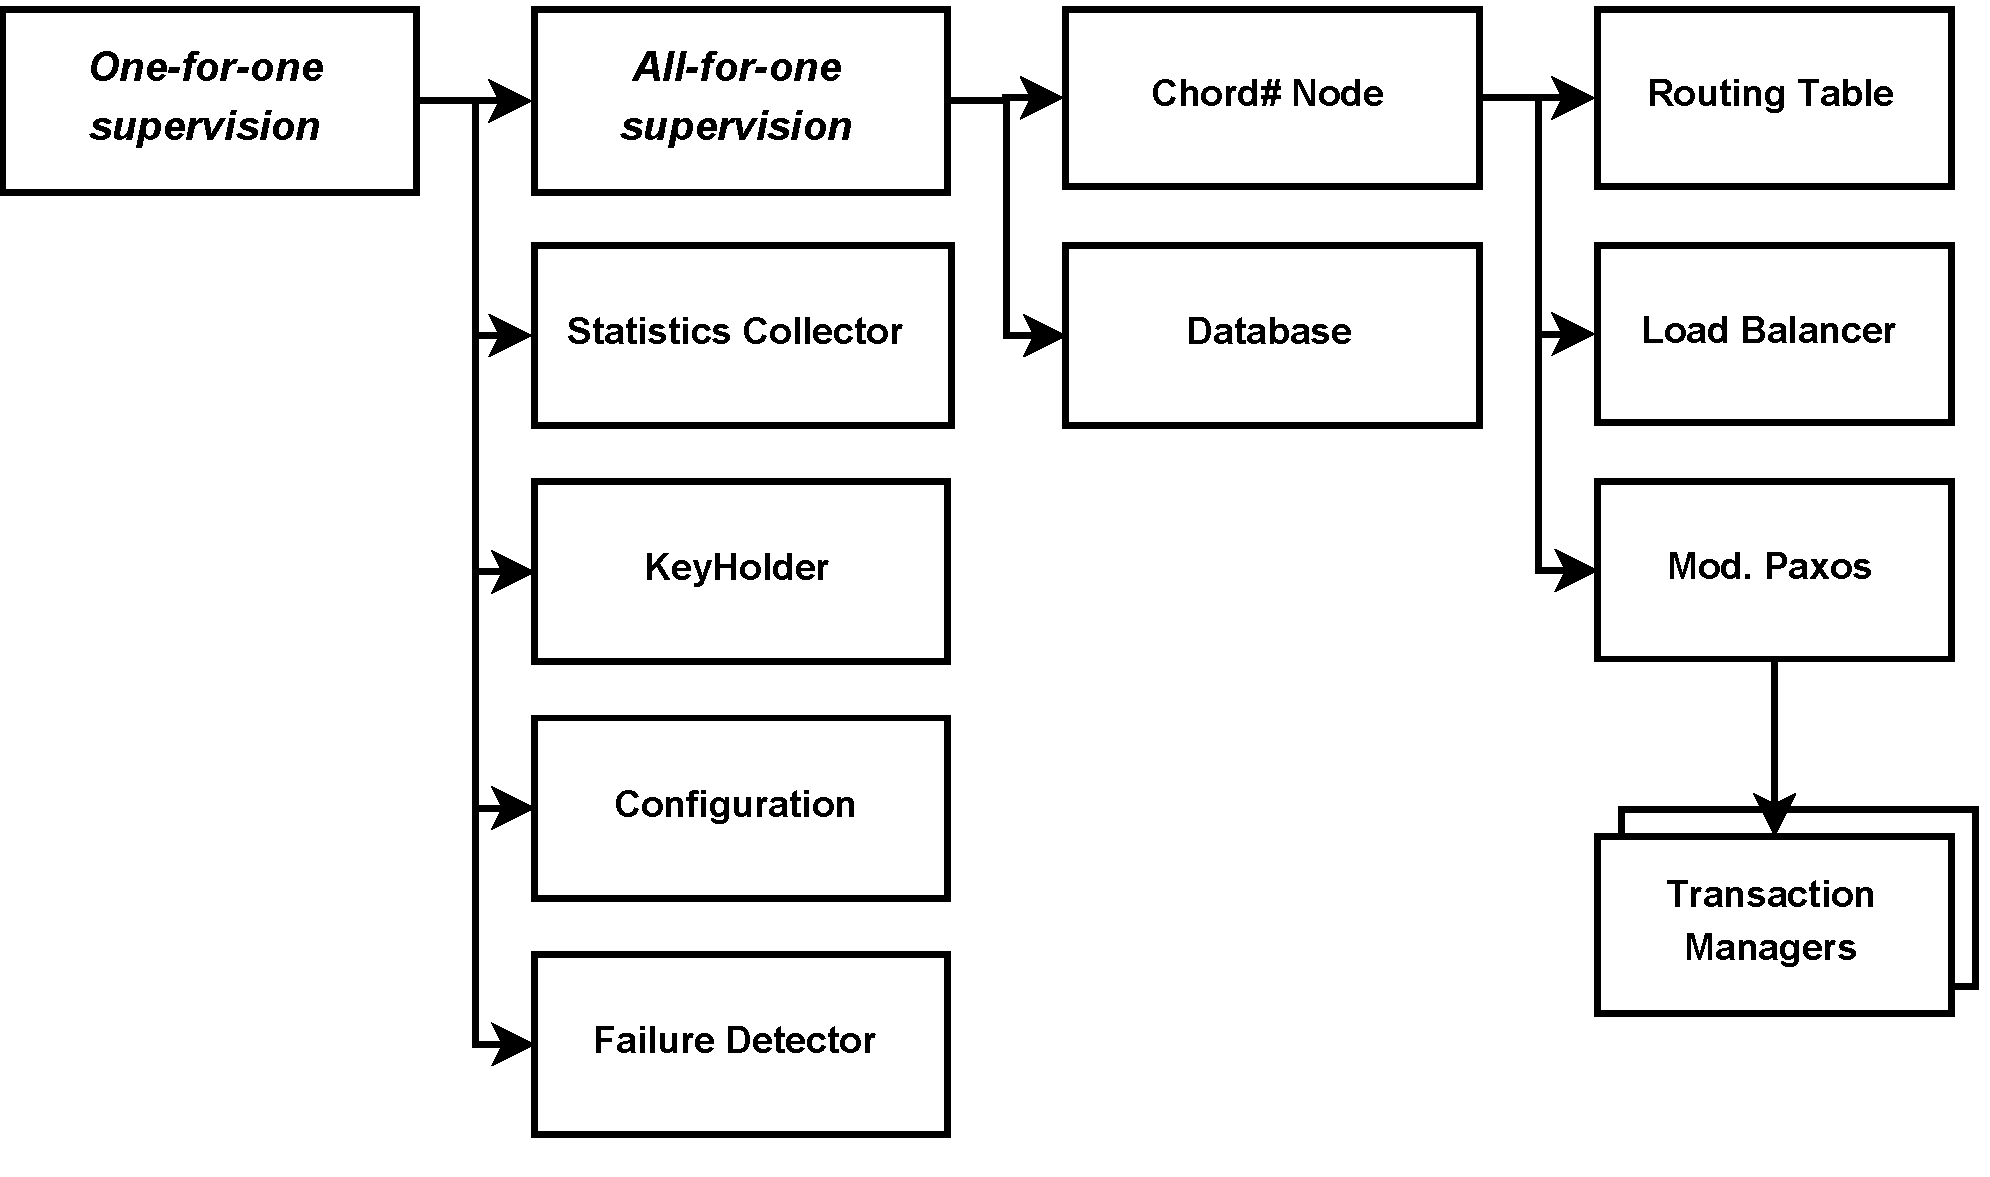
\includegraphics[width=\linewidth]{supervision}
\end{center}

When new nodes are started using \erlfun{admin}{add\_node}{/1}, only new
\code{sup_dht_node} supervisors are started.

\section{Starting the sup\_dht\_node supervisor and general processes of a node}

Starting supervisors is a two step process: a call to
\erlfun{supervisor}{start\_link}{/2,3}, e.g. from a custom supervisor's own
\code{start_link} method, will start the supervisor process. It will then
call \erlfun[]{Module}{init}{/1} to find out about the restart strategy,
maximum restart frequency and child processes.
Note that \erlfun{supervisor}{start\_link}{/2,3} will not return until
\erlfun[]{Module}{init}{/1} has returned and all child processes have been
started.

Let's have a look at \erlfun{sup\_dht\_node}{init}{/1}, the 'DHT node
supervisor'.

\codesnippet{sup_dht_node.erl}{sup_dht_node:init}{../src/sup_dht_node.erl}


The return value of the \code{init/1} function specifies the child
processes of the supervisor and how to start them. Here, we define a
list of processes to be observed by a \code{one_for_one}
supervisor. The processes are:
\code{Monitor},
\code{Delayer},
\code{Reregister},
\code{DeadNodeCache},
\code{RingMaintenance},
\code{RoutingTable},
\code{Cyclon},
\code{Vivaldi},
\code{DC_Clustering},
\code{Gossip} and a
\code{SupDHTNodeCore_AND} process in this order.

The term \code{\{one_for_one, 10, 1\}} specifies that the supervisor
should try 10 times to restart each process before giving
up. \code{one_for_one} supervision means, that if a single process
stops, only that process is restarted. The other processes run
independently.

When the \erlfun{sup\_dht\_node}{init}{/1} is finished the supervisor module
starts all the defined processes by calling the functions that were
defined in the returned list.

For a join of a new node, we are only interested in the starting of
the \code{SupDHTNodeCore_AND} process here. At that point in time, all
other defined processes are already started and running.

\section{Starting the sup\_dht\_node\_core supervisor with a peer and some paxos processes}

Like any other supervisor the \erlmodule{sup\_dht\_node\_core} supervisor
calls its \erlfun[]{sup\_dht\_node\_core}{init}{/1} function:

\codesnippet{sup_dht_node_core.erl}{sup_dht_node_core:init}{../src/sup_dht_node_core.erl}

It defines five processes, that have to be observed using a
\code{one_for_all}-supervisor, which means, that if one fails, all have to
be restarted. The \erlmodule{dht\_node} module implements the main
component of a full \scalaris{} node which glues together all the other
processes. Its
\erlfun[]{dht\_node}{start\_link}{/2} function will get
the following parameters: (a) the processes' group that is used with the \erlmodule{pid\_groups}
module and (b) a list of options for
the \erlmodule{dht\_node}. The process group name was calculated
a bit earlier in the code. \emph{Exercise: Try to find where.}


\codesnippet{dht_node.erl}{dht_node:start_link}{../src/dht_node.erl}

Like many other modules, the \erlmodule{dht\_node} module implements the
\code{gen_component}
behaviour. This behaviour was developed by us to enable us to write code which is
similar in syntax and semantics to the examples in~\cite{rachid-book}.
Similar to the \code{supervisor} behaviour, a module implementing this
behaviour has to
provide an \code{init/1} function, but here it is used to initialize the
state of the component. This function is described in the next
section.

Note: \code{?MODULE} is a predefined Erlang macro, which expands to the
module name, the code belongs to (here: \code{dht_node}).

\section{\texorpdfstring{Initializing a \code{dht_node}-process}
             {Initializing a dht\_node-process}}

\codesnippet{dht_node.erl}{dht_node:start}{../src/dht_node.erl}

The \code{gen_component} behaviour registers the \code{dht_node} in the
process dictionary. Formerly, the process had to do this itself, but
we moved this code into the behaviour. If an ID was given to
\erlfun{dht\_node}{init}{/1} function as a \code{\{\{dht_node, id\}, KEY\}}
tuple, the given Id will be used. Otherwise a random key is generated.
Depending on whether the node is the first inside a VM marked as first or not,
the according function in \erlmodule{dht\_node\_join} is called.
Also the pid of the node's supervisor is kept for future reference.

\section{Actually joining the ring}

After retrieving its identifier, the node starts the join protocol
which processes the appropriate messages calling
\erlfun{dht\_node\_join}{process\_join\_state}{Message, State}. On the
existing node, join messages will be processed by
\erlfun{dht\_node\_join}{process\_join\_msg}{Message, State}.

\subsection{A single node joining an empty ring}

\codesnippet{dht_node_join.erl}{dht_node_join:join_as_first}{../src/dht_node_join.erl}

If the ring is empty, the joining node will be the only node in the ring
and will thus be responsible for the whole key space.
It will trigger all known nodes to initialize the comm layer and then finish
the join.
\erlfun{dht\_node\_join}{finish\_join}{/5}
just creates a new state for a \scalaris{} node consisting of the given
parameters (the node as itself, its predecessor and successor,
an empty database and the queued messages that arrived during the join).
It then activates all dependent processes and creates a routing table from
this information.

The \erlfun{dht\_node\_state}{state}{} type is defined in

\codesnippet{dht_node_state.erl}{dht_node_state:state}{../src/dht_node_state.erl}

\subsection{A single node joining an existing (non-empty) ring}

If a node joins an existing ring, its join protocol will step through
the following four phases:
\begin{itemize}
  \item \makebox[4em][l]{\textbf{phase2}}
    finding nodes to contact with the help of the configured \code{known_hosts}
  \item \makebox[4em][l]{\textbf{phase2b}}
    getting the number of Ids to sample (may be skipped)
  \item \makebox[4em][l]{\textbf{phase3}}
    lookup nodes responsible for all sampled Ids
  \item \makebox[4em][l]{\textbf{phase4}}
    joining a selected node and setting up item movements
\end{itemize}

The following figure shows a (non-exhaustive) overview of the transitions
between the phases in the normal case. We will go through these step by step
and discuss what happens if errors occur.

\medskip
{\centering\documentclass[a4paper]{scrreprt}
\usepackage{typearea}
\areaset[1cm]{165mm}{240mm}

\usepackage[T1]{fontenc}
\usepackage[latin1]{inputenc}
\usepackage{listings}

\usepackage{xcolor}
\definecolor{lightyellow}{rgb}{1.0, 1.0, 0.5}
\definecolor{codebackground}{HTML}{EEEEEE}
\definecolor{commandinput}{rgb}{0.8,0.8,1}
\definecolor{lightblue}{HTML}{1E90FF}

\usepackage{tikz}
\usetikzlibrary{positioning}
\usetikzlibrary{shadows}
\usetikzlibrary{fit}
\usetikzlibrary{shapes.arrows}
\usetikzlibrary{backgrounds}
\usepackage[graphics,tightpage,active]{preview}
\PreviewEnvironment{tikzpicture}
\newlength{\imagewidth}
\newlength{\imagescale}

\usepackage{calc}

\newcommand{\code}[1]{\lstinline[basicstyle=\ttfamily]!#1!}

\begin{document}

% TODO: extend this picture and provide all paths between phases
\begin{tikzpicture}
 [rounded corners,
  pre/.style={<-,shorten <=1pt,>=stealth,semithick},
  post/.style={->,shorten >=1pt,>=stealth,semithick},
  timeout/.style={draw=black!50, dashed},
  phase/.style={rectangle,top color=black!10,bottom color=black!5},
  bend angle=60]
 \node[phase] (phase1)                         {init};
 \node[phase] (phase2)  [right=3.5 of phase1]  {phase2};
 \node[phase] (phase2b) [below=3 of phase2]    {phase2b};
 \node[phase] (phase3)  [right=3.5 of phase2]  {phase3};
 \node[phase] (phase4)  [right=3.5 of phase3]  {phase4};


 \path[->] (phase2)
             edge [pre]  node[auto, swap] {get\_known\_nodes()} (phase1)
             edge [post] node[auto, swap, align=right]
                          {
                           get\_number\_of\_samples()\\
                           \footnotesize{\textcolor{red}{skip\_psv\_lb not set,}}\\
                           \footnotesize{\textcolor{red}{non-empty ContactNodes}}
                          } (phase2b)
             edge [post] node[auto, align=left, pos=0.475]
                          {
                           lookup\_new\_ids2()\\
                           ~\footnotesize{$\hookrightarrow$lookup\_new\_ids1()}\\
                           ~~\scriptsize{$\hookrightarrow$lookup()}
                          }
                         node[auto, swap, align=left, pos=0.525]
                          {
                           \footnotesize{\textcolor{red}{skip\_psv\_lb set,}}\\
                           \footnotesize{\textcolor{red}{non-empty ContactNodes}}
                          } (phase3)
           (phase2b)
             edge [post, bend left=-35]
                         node[auto, swap, pos=0.6, align=left]
                          {
                           lookup\_new\_ids2()\\
                           ~\footnotesize{$\hookrightarrow$lookup\_new\_ids1()}\\
                           ~~\scriptsize{$\hookrightarrow$lookup()}\\
                          } (phase3)
           (phase3)
             edge [post] node[auto, align=center, pos=0.5]
                          {
                           contact\_best\_candidate()\\
                           \footnotesize{$\hookrightarrow$ send\_join\_request()}
                          } (phase4);
\end{tikzpicture}
\end{document}

}

At first all nodes set in the \code{known_hosts} configuration parameter are
contacted. Their responses are then handled in phase~2. In order to separate
the join state from the ordinary \code{dht_node} state, the
\code{gen_component} is instructed to use the \erlfun{dht\_node}{on\_join}{/2}
message handler which delegates every message to
\erlfun{dht\_node\_join}{process\_join\_state}{/2}.

\codesnippet{dht_node_join.erl}{dht_node_join:join_as_other}{../src/dht_node_join.erl}

\subsubsection{Phase 2 and 2b}

Phase~2 collects all \erlmodule{dht\_node} processes inside the contacted
VMs. It therefore mainly processes \code{get_dht_nodes_response} messages and
integrates all received nodes into the list of available connections.
The next step depends on whether the \code{\{skip_psv_lb\}} option for
skipping any passive load balancing algorithm has been
given to the \erlmodule{dht\_node} or not. If it is present, the node will
only use the ID that has been initially passed to
\erlfun{dht\_node\_join}{join\_as\_other}{/3}, issue a lookup for the
responsible
node and move to phase~3. Otherwise, the passive load balancing's
\erlfun{lb\_psv\_*}{get\_number\_of\_samples}{/1} method will be called
asking for the number of IDs to sample. Its answer will be processed in
phase~2b.

\code{get_dht_nodes_response} messages arriving in phase~2b or later will be
processed anyway and received \erlmodule{dht\_node}
processes will be integrated into the connections. These phases'
operations will not be interrupted and nothing else is changed though.

\codesnippet{dht_node_join.erl}{dht_node_join:join_other_p2}{../src/dht_node_join.erl}

Phase~2b will handle \code{get_number_of_samples} messages from the passive
load balance algorithm. Once received, new (unique) IDs will be sampled
randomly so that the total number of join candidates (selected IDs together
with fully processed candidates from further phases) is at least as high as
the given number of samples. Afterwards, lookups will be created for all
previous IDs as well as the new ones and the node will move to phase~3.

\codesnippet{dht_node_join.erl}{dht_node_join:join_other_p2b}{../src/dht_node_join.erl}

Lookups will make \scalaris{} find the node currently responsible for a given ID
and send a request to simulate a join to this node, i.e. a
\code{get_candidate} message. Note that during such an operation, the joining
node would become the existing node's predecessor. The simulation will be
delegated to the passive load balance algorithm the joining node requested, as
set by the \code{join_lb_psv} configuration parameter. 

\codesnippet{dht_node_join.erl}{dht_node_join:get_candidate}{../src/dht_node_join.erl}

\subsubsection{Phase 3}

The result of the simulation will be send in a \code{get_candidate_response}
message and will be processed in phase~3 of the joining node. It will be
integrated into the list of processed candidates. If there are no more IDs
left to process, the best among them will be contacted. Otherwise further
\code{get_candidate_response} messages will be awaited.
Such messages will also be processed in the other phases where the candidate
will be simply added to the list.

\codesnippet{dht_node_join.erl}{dht_node_join:join_other_p3}{../src/dht_node_join.erl}

If \erlfun{dht\_node\_join}{contact\_best\_candidate}{/1} is called and
candidates are available (there should be at this stage!), it will sort the
candidates by using the passive load balance algorithm, send a 
\code{join_request} message and continue with phase~4. 

\erlfunindex{dht\_node\_join}{contact\_best\_candidate}
\codesnippet{dht_node_join.erl}{dht_node_join:contact_best_candidate}{../src/dht_node_join.erl}
\erlfunindex{dht\_node\_join}{send\_join\_request}
\codesnippet{dht_node_join.erl}{dht_node_join:send_join_request}{../src/dht_node_join.erl}

The \code{join_request} message will be received by the existing node which
will set up a slide operation with the new node. If it is not responsible for
the key (anymore), it will deny the request and reply with a
\code{\{join, join_response, not_responsible, Node\}} message.
If it is responsible for the ID and is not participating in a slide with its
current predecessor, it will set up a slide with the joining node:

\codesnippet{dht_node_join.erl}{dht_node_join:join_request1}{../src/dht_node_join.erl}

\subsubsection{Phase 4}

The joining node will receive the \code{join_response} message in phase~4 of
the join protocol. If everything is ok, it will
notify its ring maintenance process that it enters the ring, start all required
processes and join the slide operation set up by the existing node in order to
receive some of its data.

If the join candidate's node is not responsible for the candidate's ID anymore
or the candidate's ID already exists, the next candidate is contacted until
no further candidates are available and the join protocol starts over using
\erlfun{dht\_node\_join}{start\_over}{/1}.

Note that the \code{join_response} message will actually be processed in
any phase. Therefore, if messages arrive late, the join can be processed
immediately and the rest of the join protocol does not need to be executed
again.

\codesnippet{dht_node_join.erl}{dht_node_join:join_other_p4}{../src/dht_node_join.erl}
\erlfunindex{dht\_node\_join}{finish\_join}
\erlfunindex{dht\_node\_join}{finish\_join\_and\_slide}
\codesnippet{dht_node_join.erl}{dht_node_join:finish_join}{../src/dht_node_join.erl}

The macro \code{?RT} maps to the configured routing algorithm. It is defined
in \code{include/scalaris.hrl}. For further details on the routing see
Chapter~\sieheref{chapter.routing}.

\subsubsection{Timeouts and other errors}

The following table summarizes the timeout messages send during the join
protocol on the joining node. It shows in which of the phases each of the
messages is processed and describes (in short) what actions are taken.
All of these messages are influenced by their respective config parameters,
e.g. \code{join_timeout} parameter in the config files defines an overall
timeout for the whole join operation. If it takes longer than
\code{join_timeout} ms, a \code{\{join, timeout\}} will be send and processed
as given in this table.

\medskip
{\small
\begin{tabular}{lP{2.4cm}P{2.75cm}P{2.35cm}P{3.25cm}M{1.70cm}}
  \toprule
  & \code{known_hosts}\carriagereturn\newline\code{_timeout}
  & \code{get_number_of}\carriagereturn\newline\code{_samples}\carriagereturn\newline\code{_timeout}
  & \code{lookup}\carriagereturn\newline\code{ _timeout}
  & \code{join_request}\carriagereturn\newline\code{_timeout}
  & \code{timeout} \tn
  \midrule
  %
  \bfseries phase2
  & get known nodes from configured VMs
  & ignore
  & ignore
  & ignore
  & \multirow{21}{1.70cm}
        {re-start join\newline$\rightarrow$ phase~2 or 2b} \tn
  \cmidrule(r){1-5}
  %
  \bfseries phase2b
  & ignore
  & remove contact node, re-start join\newline
    $\rightarrow$ phase~2 or 2b
  & ignore
  & ignore
  & \tn
  \cmidrule(r){1-5}
  %
  \bfseries phase3
  & ignore
  & ignore
  & remove contact node, lookup remaining IDs\newline
    $\rightarrow$ phase~2 or 3 
  & ignore
  & \tn
  \cmidrule(r){1-5}
  %
  \bfseries phase3b
  & ignore
  & ignore
  & ignore
  & ignore
  & \tn
  \cmidrule(r){1-5}
  %
  \bfseries phase4
  & ignore
  & ignore
  & ignore
  & timeouts $< 3$?\footnote{set by the \code{join_request_timeouts} config parameter}\newline
    \mbox{}~$\rightarrow$ contact candidate\newline
    otherwise:\newline
    \mbox{}~remove candidate\newline
    \mbox{}~no candidates left?\newline
    \mbox{}~~$\rightarrow$ phase~2 or 2b\newline
    \mbox{}~otherwise:\newline
    \mbox{}~~$\rightarrow$ contact next one\newline
    \mbox{}~~$\rightarrow$ phase~3b or 4
  & \tn
  \bottomrule
\end{tabular}
}
\medskip

On the existing node, there is only one timeout message which is part of the
join protocol: the \code{join_response_timeout}. It will be send when a slide
operation is set up and if the timeout hits before the next message exchange,
it will increase the slide operation's number of timeouts. The slide will be
aborted if at least \code{join_response_timeouts} timeouts have been received.
This parameter is set in the config file.

\subsubsection{Misc. (all phases)}

Note that join-related messages arriving in other phases than those handling
them will be ignored. Any other messages during a \code{dht_node}'s join will
be queued and re-send when the join is complete.

\chapter{How data is transferred (atomically)}
\label{chapter.slide}
\svnrev{r4750}

A data transfer from a node to one of its (two) neighbours is also called a
\emph{slide}. A slide operation is defined in the \erlmodule{slide\_op} module,
the protocol is mainly implemented in \erlmodule{dht\_node\_move}.
Parts of the slide are dependent on the ring maintenance implementation and are
split off into modules implementing the \erlmodule{slide\_beh} behaviour.

Though the protocols are mainly symmetric, we distinguish between sending data
to the predecessor and sending data to the successor, respectively. In the
following protocol visualisations, arrows denote message exchanges, pseudo-code
for operations that are being executed is put at the side of each time bar.
Functions in green are those implemented in the \erlmodule{slide\_beh}
behaviour, if annotated with an arrow pointing to itself, this callback is
asynchronous.
During the protocol, the slide operation goes through several phases which are
show in black boxes.

In general, a slide consists of three steps:
\begin{enumerate}
 \item set up slide
 \item send data \& start recording changes, i.e. delta
 \item send delta \& transfer responsibility
\end{enumerate}

The latter two may be repeated to execute incremental slides which further
reduce periods of unavailability. During this period, no node is responsible
for the range to transfer and messages are thus delayed until the receiving
node gains responsibility.

%\pagebreak
\section{Sending data to the predecessor}

\subsection{Protocol}
\documentclass[a4paper]{scrreprt}
\usepackage{typearea}
\areaset[1cm]{165mm}{240mm}

\usepackage[T1]{fontenc}
\usepackage[latin1]{inputenc}
\usepackage{listings}

\usepackage{xcolor}
\definecolor{lightyellow}{rgb}{1.0, 1.0, 0.5}
\definecolor{codebackground}{HTML}{EEEEEE}
\definecolor{commandinput}{rgb}{0.8,0.8,1}
\definecolor{lightblue}{HTML}{1E90FF}

\usepackage{tikz}
\usetikzlibrary{positioning}
\usetikzlibrary{shadows}
\usetikzlibrary{fit}
\usetikzlibrary{shapes.arrows}
\usetikzlibrary{backgrounds}
\usepackage[graphics,tightpage,active]{preview}
\PreviewEnvironment{tikzpicture}
\newlength{\imagewidth}
\newlength{\imagescale}

\usepackage{calc}

\newcommand{\code}[1]{\lstinline[basicstyle=\ttfamily]!#1!}

\begin{document}


\newlength{\tikzinnerheight}
\setlength{\tikzinnerheight}{1.0cm}
\newlength{\tikzsepheight}
\setlength{\tikzsepheight}{0.75cm}
\newlength{\tikzstartsecond}
\setlength{\tikzstartsecond}{0cm}
\newlength{\tikzstartfirst}
\setlength{\tikzstartfirst}{\tikzstartsecond + \tikzinnerheight + 0.5\tikzsepheight}
\newlength{\tikzsepinner}
\setlength{\tikzsepinner}{\tikzinnerheight + \tikzsepheight}
% \newlength{\tikzendsucc}
% \setlength{\tikzendsucc}{\tikzsepinner + \tikzstartfirst - \tikzstartsecond}

\begin{tikzpicture}
 [pre/.style={<-,shorten <=1pt,>=stealth,semithick},
  post/.style={->,shorten >=1pt,>=stealth,semithick},
  progress/.style={-,dashed,thin,black},
  timeout/.style={draw=black!50, dashed},
  process/.style={rectangle,black,rounded corners},
  start/.style={rectangle,draw,thick,fill=yellow,draw=black,minimum height=0.7cm},
  inner/.style={minimum height=\tikzinnerheight,thin},
  end/.style={minimum height=0.4cm},
  phase/.style={rectangle,draw,thick,black},
  my_node/.style={rectangle,fill=codebackground,drop shadow,rounded corners},
  action_l/.style={rectangle,black,font=\footnotesize,align=right},
  action_r/.style={rectangle,black,font=\footnotesize,align=left},
  note/.style={circle, thin, draw, outer sep=0.1cm},
  async_r/.style={post,min distance=0.5,looseness=2.5,in=0,out=0},
  async_l/.style={post,min distance=0.5,looseness=2.5,in=180,out=180},
  async_desc/.style={rectangle,black,font=\footnotesize},
  msg/.style={sloped},
  msg_t/.style={msg,anchor=south},
  msg_b/.style={msg,anchor=north},
  bend angle=60]

 \node[font={\Large\bfseries}] (heading1) {Send data to predecessor};
 \node[font=\footnotesize,below=-0.2 of heading1] (heading2) {(version 2.0)};

 \node[start] (pred)      [below left=0.5 and 2.5 of heading1.south] {pred};
 \node[inner] (pred-init)           [below=\tikzstartfirst of pred]      {};
 \node[inner] (pred-got-data)       [below=\tikzsepinner of pred-init] {};
 \node[inner] (pred-got-delta)      [below=\tikzsepinner of pred-got-data] {};
 \node[inner] (pred-got-owner)      [below=\tikzsepinner of pred-got-delta] {};
 \node[end]   (pred-end)  [below=\tikzstartsecond of pred-got-owner] {\footnotesize pred};

 \node[start] (succ)      [below right=0.5 and 2.5 of heading1.south] {succ};
 \node[inner] (succ-init)           [below=\tikzstartsecond of succ]      {};
 \node[inner] (succ-send-data)      [below=\tikzsepinner of succ-init]      {};
 \node[inner] (succ-send-delta)     [below=\tikzsepinner of succ-send-data]      {};
 \node[inner] (succ-send-owner)     [below=\tikzsepinner of succ-send-delta]      {};
 \node[end]   (succ-end)  [below=\tikzstartfirst of succ-send-owner] {\footnotesize succ};

 \path[-] (pred)
            edge [progress] (pred-end)
          (succ)
            edge [progress] (succ-end);

 \path[->] (succ-init.south west)
             edge [post,draw=lightgray] node[msg_t, lightgray,font=\footnotesize] {slide, pred, 'send'} node[msg_b, lightgray,font=\footnotesize] {(optional)} (pred-init.north east)
           (pred-init.south east)
             edge [post]  node[msg_t] {slide, succ, 'rcv'\textcolor{lightgray}{, MaxE}} (succ-send-data.north west)

           (succ-send-data.east)
             edge [async_r] node[async_desc, auto, anchor=west] {\textcolor{green}{prepare\_send\_data(SlideOp)}}
                  (succ-send-data.south east)

           (succ-send-data.south west)
             edge [post] node[msg_t] {data\textcolor{lightgray}{, TargetId, NextOp}} (pred-got-data.north east)
           (pred-got-data.south east)
             edge [post] node[msg_t] {data\_ack} (succ-send-delta.north west)

           (pred-got-data.north west)
             edge [async_l] node[async_desc, auto, anchor=east] {\textcolor{green}{update\_rcv\_data(SlideOp, TargetId, NextOp)}}
                  (pred-got-data.west)

           (succ-send-delta.north east)
             edge [async_r] node[async_desc, auto, anchor=west] {\textcolor{green}{prepare\_send\_selta(SlideOp)}}
                  (succ-send-delta.east)

           (succ-send-delta.south west)
             edge [post] node[msg_t] {delta} (pred-got-delta.north east)
           (pred-got-delta.south east)
             edge [post] node[msg_t] {delta\_ack} (succ-send-owner.north west)

           (succ-send-owner.north east)
             edge [async_r] node[async_desc, auto, anchor=west] (update_owner) {\textcolor{green}{update\_owner(SlideOp)}}
                  (succ-send-owner.east);


 \node[action_l, left=0.1 of pred-init.east] {
   SlideOp.new()\\
   fd.subscribe(SlideOp.node)\\
   \textcolor{green}{prepare\_rcv\_data(SlideOp)}%
 };
 \node[phase, below left=0.35 and 0.1 of pred-init.south] (pred-init-p-leases) {wait\_for\_data};

 \node[phase, below left=0.1 and 0.1 of pred-got-data.south] {wait\_for\_delta};

 \node[action_l, left=0.1 of pred-got-delta.east] {
   \textcolor{green}{finish\_delta(SlideOp)}\\
   fd.unsubscribe(SlideOp.node)\\
   SlideOp.delete()%
 };

 \node[action_l, left=0.1 of pred-got-owner.east] {}; % nothing to do



 \node[action_r, right=0.1 of succ-init.south west, lightgray] {
   SlideOp.new()\\
   fd.subscribe(SlideOp.node)%
 };
 \node[phase, below right=0.4 and 0.1 of succ-init.south, lightgray] {wait\_for\_other};

 \node[action_r, right=0.1 of succ-send-data.north west,anchor=west] {
   SlideOp.new()\\
   fd.subscribe(SlideOp.node)%
 };

 \node[action_r, below=0.3 of succ-send-data.south,anchor=west] {
   db.record\_changes(SlideOp.interval)%
 };
 \node[phase, below right=0.5 and 0.1 of succ-send-data.south] {wait\_for\_data\_ack};

 \node[action_r, below right=0.1 and 0.1 of succ-send-delta.south west, anchor=south west] {
   db.stop\_record\_changes(SlideOp.interval)%
 };
 \node[phase, below right=0.1 and 0.1 of succ-send-delta.south] {wait\_for\_delta\_ack};

 \coordinate (succ-cont-start1) at ($(succ-send-owner)-(0,.5\tikzsepinner)$);
 \coordinate (succ-cont-end) at ($(succ-send-data)+(0,0.1)$);
 \coordinate (pred-cont-start1) at ($(pred-got-delta.south)+(0,-0.25)$);
 \coordinate (pred-cont-start2) at ($(pred-cont-start1)-(0,1.25)$);
 \coordinate (pred-cont-end) at ($(pred-init.south)+(0,-0.25)$);

 \path[->] (update_owner.south west)
             edge [async_r,draw=lightgray,dashed,out=-50,in=150,looseness=0.8] node[msg_t, pos=0.5, lightgray, font=\footnotesize] {rm\_update} node[msg_b, pos=0.5, lightgray, font=\footnotesize] {(to dht\_node)} node[pos=0.37,note,draw,red,anchor=north] {$\ell$} ($(pred-cont-start1)!0.7!(pred-cont-start2)$);

 \draw[post, rounded corners, dashed, lightgray] (succ-cont-start1) -- +(7,0) -- ($(succ-cont-end)+(7,0)$) -- (succ-cont-end);
 \node[action_l, lightgray, anchor=south east] at ($(succ-cont-start1)+(7,0)$) {if (NextOp == continue)\\SlideOp.update()};

 \node[action_r, below right=\tikzstartfirst and 0.1 of succ-send-owner.north west, anchor=north west] {
   fd.unsubscribe(SlideOp.node)\\
   SlideOp.delete()%
 };

 \coordinate (pred-cont-mid) at ($(pred-cont-start1)+(-7.5,0.2)$);
 \draw[post, rounded corners, dashed, lightgray] (pred-cont-start1) -- +(-7.5,0) -- ($(pred-cont-end)+(-7.5,0)$) -- (pred-cont-end);
 \draw[post, rounded corners, dashed, lightgray] (pred-cont-start2) -- +(-7.5,0) -- (pred-cont-mid);
 \node[action_r, lightgray, anchor=west] at ($(pred-cont-start1)!0.5!(pred-cont-start2)+(-7.5,0)$) {if (NextOp == continue) -> continue\\SlideOp.update()\\prepare\_rcv\_data(SlideOp)};

\end{tikzpicture}
\end{document}


\subsection{Callbacks}
% \medskip
{%\small
\begin{tabular}{P{4.2cm}P{5.4cm}P{5.4cm}}
  \toprule
  & \code{slide_chord}
  & \code{slide_leases} \tn
  \midrule
  %
  \bfseries $\leftarrow$ prepare\_rcv\_data
  & \emph{\color{gray}nothing to do}
  & \emph{\color{gray}nothing to do} \tn
  \midrule
  %
  \bfseries $\rightarrow$ prepare\_send\_data
  & add DB range
  & \emph{\color{gray}nothing to do} \tn
  \midrule
  %
  \bfseries $\leftarrow$ update\_rcv\_data
  & set MSG forward,\\change my ID
  & \emph{\color{gray}nothing to do} \tn
  \midrule
  %
  \bfseries $\rightarrow$ prepare\_send\_delta
  & wait until pred up-to-date,\\then: remove DB range
  & split own lease into two ranges, locally disable lease sent to pred \tn
  \midrule
  %
  \bfseries $\leftarrow$ finish\_delta
  & remove MSG forward
  & \emph{\color{gray}nothing to do} \tn
  \midrule
  %
  \bfseries $\rightarrow$ finish\_delta\_ack
  & \emph{\color{gray}nothing to do}
  & hand over the lease to pred, notify pred of owner change \tn
  \bottomrule
\end{tabular}
}
% \medskip

\pagebreak
\section{Sending data to the successor}

\subsection{Protocol}
\documentclass[a4paper]{scrreprt}
\usepackage{typearea}
\areaset[1cm]{165mm}{240mm}

\usepackage[T1]{fontenc}
\usepackage[latin1]{inputenc}
\usepackage{listings}

\usepackage{xcolor}
\definecolor{lightyellow}{rgb}{1.0, 1.0, 0.5}
\definecolor{codebackground}{HTML}{EEEEEE}
\definecolor{commandinput}{rgb}{0.8,0.8,1}
\definecolor{lightblue}{HTML}{1E90FF}

\usepackage{tikz}
\usetikzlibrary{positioning}
\usetikzlibrary{shadows}
\usetikzlibrary{fit}
\usetikzlibrary{shapes.arrows}
\usetikzlibrary{backgrounds}
\usepackage[graphics,tightpage,active]{preview}
\PreviewEnvironment{tikzpicture}
\newlength{\imagewidth}
\newlength{\imagescale}

\usepackage{calc}

\newcommand{\code}[1]{\lstinline[basicstyle=\ttfamily]!#1!}

\begin{document}


\newlength{\tikzinnerheight}
\setlength{\tikzinnerheight}{1.0cm}
\newlength{\tikzsepheight}
\setlength{\tikzsepheight}{0.75cm}
\newlength{\tikzstartsecond}
\setlength{\tikzstartsecond}{0cm}
\newlength{\tikzstartfirst}
\setlength{\tikzstartfirst}{\tikzstartsecond + \tikzinnerheight + 0.5\tikzsepheight}
\newlength{\tikzsepinner}
\setlength{\tikzsepinner}{\tikzinnerheight + \tikzsepheight}
% \newlength{\tikzendsucc}
% \setlength{\tikzendsucc}{\tikzsepinner + \tikzstartfirst - \tikzstartsecond}

\begin{tikzpicture}
 [pre/.style={<-,shorten <=1pt,>=stealth,semithick},
  post/.style={->,shorten >=1pt,>=stealth,semithick},
  progress/.style={-,dashed,thin,black},
  timeout/.style={draw=black!50, dashed},
  process/.style={rectangle,black,rounded corners},
  start/.style={rectangle,draw,thick,fill=yellow,draw=black,minimum height=0.7cm},
  inner/.style={minimum height=\tikzinnerheight,thin},
  end/.style={minimum height=0.4cm},
  phase/.style={rectangle,draw,thick,black},
  my_node/.style={rectangle,fill=codebackground,drop shadow,rounded corners},
  action_l/.style={rectangle,black,font=\footnotesize,align=right},
  action_r/.style={rectangle,black,font=\footnotesize,align=left},
  note/.style={circle, thin, draw, outer sep=0.1cm},
  async_r/.style={post,min distance=0.5,looseness=2.5,in=0,out=0},
  async_l/.style={post,min distance=0.5,looseness=2.5,in=180,out=180},
  async_desc/.style={rectangle,black,font=\footnotesize},
  msg/.style={sloped},
  msg_t/.style={msg,anchor=south},
  msg_b/.style={msg,anchor=north},
  bend angle=60]

 \node[font={\Large\bfseries}] (heading1) {Send data to successor};
 \node[font=\footnotesize,below=-0.2 of heading1] (heading2) {(version 2.0)};

 \node[start] (pred)      [below left=0.5 and 2.5 of heading1.south] {pred};
 \node[inner] (pred-init)           [below=\tikzstartsecond of pred]      {};
 \node[inner] (pred-send-data)      [below=\tikzsepinner of pred-init] {};
 \node[inner] (pred-send-delta)     [below=\tikzsepinner of pred-send-data] {};
 \node[inner] (pred-send-owner)     [below=\tikzsepinner of pred-send-delta] {};
 \node[end]   (pred-end)  [below=\tikzstartfirst of pred-send-owner] {\footnotesize pred};

 \node[start] (succ)      [below right=0.5 and 2.5 of heading1.south] {succ};
 \node[inner] (succ-init)           [below=\tikzstartfirst of succ]      {};
 \node[inner] (succ-got-data)      [below=\tikzsepinner of succ-init]      {};
 \node[inner] (succ-got-delta)     [below=\tikzsepinner of succ-got-data]      {};
 \node[inner] (succ-got-owner)      [below=\tikzsepinner of succ-got-delta] {};
 \node[end]   (succ-end)  [below=\tikzstartsecond of succ-got-owner] {\footnotesize succ};

 \path[-] (pred)
            edge [progress] (pred-end)
          (succ)
            edge [progress] (succ-end);

 \path[->] (pred-init.south east)
             edge [post,lightgray]  node[msg_t,lightgray,font=\footnotesize] {slide, succ, 'send'} node[msg_b,lightgray,font=\footnotesize] {(optional)} (succ-init.north west)
           (succ-init.south west)
             edge [post] node[msg_t] {slide, pred, 'rcv'\textcolor{lightgray}{, MaxE}} (pred-send-data.north east)

           (pred-send-data.west)
             edge [async_l] node[async_desc, auto, anchor=east, align=right] {\textcolor{green}{prepare\_send\_data(SlideOp)}}
                  (pred-send-data.south west)

           (pred-send-data.south east)
             edge [post] node[msg_t] {data\textcolor{lightgray}{, TargetId, NextOp}} (succ-got-data.north west)
           (succ-got-data.south west)
             edge [post] node[msg_t] {data\_ack} (pred-send-delta.north east)

           (pred-send-delta.north west)
             edge [async_l] node[async_desc, auto, anchor=east] {\textcolor{green}{prepare\_send\_selta(SlideOp)}}
                  (pred-send-delta.west)

           (pred-send-delta.south east)
             edge [post] node[msg_t] {delta} (succ-got-delta.north west)
           (succ-got-delta.south west)
             edge [post] node[msg_t] {delta\_ack} (pred-send-owner.north east)

           (pred-send-owner.north west)
             edge [async_l] node[async_desc, auto, anchor=east] (update_owner) {\textcolor{green}{update\_owner(SlideOp)}}
                  (pred-send-owner.west);


 \node[action_l, left=0.1 of pred-init.south east ,lightgray] {
   SlideOp.new()\\
   fd.subscribe(SlideOp.node)%
 };
 \node[phase, below left=0.4 and 0.1 of pred-init.south, lightgray] {wait\_for\_other};

 \node[action_l, left=0.1 of pred-send-data.north east] {
   SlideOp.new()\\
   fd.subscribe(SlideOp.node)%
 };
 
 \node[action_l, left=0.1 of pred-send-data.south east, anchor=north east] {
   db.record\_changes(SlideOp.interval)%
 };
 \node[phase, below left=0.5 and 0.1 of pred-send-data.south] {wait\_for\_data\_ack};
 
 \node[action_l, below left=0.1 and 0.1 of pred-send-delta.south east, anchor=south east] {
   db.stop\_record\_changes(SlideOp.interval)%
 };
 \node[phase, below left=0.1 and 0.1 of pred-send-delta.south] {wait\_for\_delta\_ack};


 
 \node[action_r, right=0.1 of succ-init.west] {
   SlideOp.new()\\
   fd.subscribe(SlideOp.node)\\
   \textcolor{green}{prepare\_rcv\_data(SlideOp)}%
 };
 \node[phase, below right=0.35 and 0.1 of succ-init.south] {wait\_for\_data};

 \node[action_r, right=0.1 of succ-got-data.west] {
   \textcolor{green}{update\_rcv\_data(SlideOp, TargetId, NextOp)}%
 };
 \node[phase, below right=0.1 and 0.1 of succ-got-data.south] {wait\_for\_delta};

 \node[action_r, right=0.1 of succ-got-delta.west] {
   \textcolor{green}{finish\_delta(SlideOp)}%
 };

 \node[action_r, right=0.1 of succ-got-owner.west] {}; % nothing to do

 \coordinate (succ-cont-start1) at ($(succ-got-delta.south)-(0,0.25)$);
 \coordinate (succ-cont-start2) at ($(succ-cont-start1)-(0,1.25)$);
 \coordinate (succ-cont-end) at ($(succ-init.south)+(0,-0.25)$);
 \coordinate (pred-cont-start1) at ($(pred-send-owner)-(0,.5\tikzsepinner)$);
 \coordinate (pred-cont-end) at ($(pred-send-data.west)+(0,0.1)$);

 \path[->] (update_owner.south east)
             edge [async_l,draw=lightgray,dashed,out=230,in=30,looseness=0.8] node[msg_t, pos=0.5, lightgray, font=\footnotesize] {rm\_update} node[msg_b, pos=0.5, lightgray, font=\footnotesize] {(to dht\_node)} node[pos=0.37,note,draw,red,anchor=north] {$\ell$} ($(succ-cont-start1)!0.7!(succ-cont-start2)$);

 \draw[post, rounded corners, dashed, lightgray] (pred-cont-start1) -- +(-7,0) -- ($(pred-cont-end)+(-7,0)$) -- (pred-cont-end);
 \node[action_r, lightgray, anchor=south west] at ($(pred-cont-start1)+(-7,0)$) {if (NextOp == continue)\\SlideOp.update()};

 \node[action_l, below left=\tikzstartfirst and 0.1 of pred-send-owner.north east, anchor=north east] {
   fd.unsubscribe(SlideOp.node)\\
   SlideOp.delete()%
 };
 
 \coordinate (succ-cont-mid) at ($(succ-cont-start1)+(7,0.2)$);
 \draw[post, rounded corners, dashed, lightgray] (succ-cont-start1) -- +(7,0) -- ($(succ-cont-end)+(7,0)$) -- (succ-cont-end);
 \draw[post, rounded corners, dashed, lightgray] (succ-cont-start2) -- +(7,0) -- (succ-cont-mid);
 \node[action_l, lightgray, anchor=east] at ($(succ-cont-start1)!0.5!(succ-cont-start2)+(7,0)$) {if (NextOp == continue) -> continue\\SlideOp.update()\\prepare\_rcv\_data(SlideOp)};

 \node[action_r, below right=\tikzstartsecond and 0.1 of succ-got-owner.north west, anchor=north west] {
   fd.unsubscribe(SlideOp.node)\\
   SlideOp.delete()%
 };

\end{tikzpicture}
\end{document}


\subsection{Callbacks}

% \medskip
{%\small
\begin{tabular}{P{4.2cm}P{5.4cm}P{5.4cm}}
  \toprule
  & \code{slide_chord}
  & \code{slide_leases} \tn
  \midrule
  %
  \bfseries $\rightarrow$ prepare\_rcv\_data
  & set MSG forward
  & \emph{\color{gray}nothing to do} \tn
  \midrule
  %
  \bfseries $\leftarrow$ prepare\_send\_data
  & add DB range,\\change my ID
  & \emph{\color{gray}nothing to do} \tn
  \midrule
  %
  \bfseries $\rightarrow$ update\_rcv\_data
  & \emph{\color{gray}nothing to do}
  & \emph{\color{gray}nothing to do} \tn
  \midrule
  %
  \bfseries $\leftarrow$ prepare\_send\_delta
  & remove DB range
  & split own lease into two ranges, locally disable lease sent to succ \tn
  \midrule
  %
  \bfseries $\rightarrow$ finish\_delta
  & remove MSG forward,\\until pred up-to-date:\\$\hookrightarrow$ add DB range\\then: remove DB range
  & \emph{\color{gray}nothing to do} \tn
  \midrule
  %
  \bfseries $\leftarrow$ finish\_delta\_ack
  & \emph{\color{gray}nothing to do}
  & hand over the lease to succ, notify succ of owner change \tn
  \bottomrule
\end{tabular}
}
% \medskip

\chapter{Directory Structure of the Source Code}

The directory tree of \scalaris{} is structured as follows:

\vspace*{1em}
\begin{tabular}{|r|p{11.5cm}|}
 \hline
 \code{bin} & contains shell scripts needed to work with \scalaris{} (e.g.\ start the management server, start a node, \dots)\\
 \code{contrib} & necessary third party packages (yaws and log4erl) \\
 \code{doc} & generated Erlang documentation \\
 \code{docroot} & root directory of the node's webserver \\
 \code{ebin} & the compiled Erlang code (beam files)\\
 \code{java-api} & a Java API to \scalaris{} \\
 \code{log} & log files \\
 \code{src} & contains the \scalaris{} source code\\
 \code{test} & unit tests for \scalaris{} \\
 \code{user-dev-guide} & contains the sources for this document\\
 \hline
\end{tabular}


%\chapter{System Components}

%\chapter{Processes}

%\chapter{Troubleshooting}

%\section{ApplicationMonitor appmon:start()}

\chapter{Java API}

For the Java API documentation, we refer the reader to the documentation
generated by javadoc or doxygen. The following commands create the
documentation:

\begin{lstlisting}[language=sh]
%> cd java-api
%> ant doc
%> doxygen
\end{lstlisting}

The documentation can then be found in \code{java-api/doc/index.html}
(javadoc) and\\ \code{java-api/doc-doxygen/html/index.html} (doxygen).

The API is divided into four classes:

\begin{itemize}
\item \code{de.zib.scalaris.Transaction} for (multiple) operations inside a
       transaction
\item \code{de.zib.scalaris.TransactionSingleOp} for single transactional
       operations
\item \code{de.zib.scalaris.ReplicatedDHT} for non-transactional (inconsistent)
       access to the replicated DHT items, e.g. deleting items
\item \code{de.zib.scalaris.PubSub} for topic-based publish/subscribe
       operations
\end{itemize}


\bibliographystyle{plainnat}

\begin{thebibliography}{9}

\bibitem{erlang-book}
Joe Armstrong.
\newblock \emph{Programming Erlang: Software for a Concurrent World.}
\newblock Pragmatic Programmers, ISBN: 978-1-9343560-0-5, July 2007

\bibitem{vivaldi}
Frank Dabek, Russ Cox, Frans Kaahoek, Robert Morris.
\newblock \emph{Vivaldi: A Decentralized Network Coordinate System.}
\newblock ACM SIGCOMM 2004.

\bibitem{rachid-book}
Rachid Guerraoui and Luis Rodrigues.
\newblock \emph{Introduction to Reliable Distributed Programming.}
\newblock Springer-Verlag, 2006.

\bibitem{chord-sigcomm}
Ion Stoica, Robert Morris, David Karger, M. Frans Kaashoek and Hari Balakrishnan.
\newblock \emph{Chord: A Scalable Peer-to-peer Lookup Service for Internet Applications.}
\newblock ACM SIGCOMM 2001, San Deigo, CA, August 2001, pp. 149-160.
\newblock \href{http://pdos.csail.mit.edu/papers/chord:sigcomm01/chord_sigcomm.pdf}{http://pdos.csail.mit.edu/papers/chord:sigcomm01/chord\_sigcomm.pdf}

\bibitem{t-man}
M{\'a}rk Jelasity, Alberto Montresor, Ozalp Babaoglu.
\newblock \emph{T-Man: Gossip-based fast overlay topology construction.}
\newblock Computer Networks (CN) 53(13):2321-2339, 2009.

\bibitem{frtchord}
  Hiroya Nagao, Kazuyuki Shudo.
  \newblock \emph{Flexible routing tables: Designing routing
    algorithms for overlays based on a total order on a routing table set.}
  \newblock In: Peer-to-Peer Computing, IEEE, 2011.

\bibitem{enhanced-paxos}
F. Schintke, A. Reinefeld, S. Haridi, T. Sch{\"u}tt.
\newblock \emph{Enhanced Paxos Commit for Transactions on DHTs.}
\newblock 10th IEEE/ACM Int. Conf. on Cluster, Cloud and Grid Computing, pp. 448-454,
May 2010.

\bibitem{cyclon}
Spyros Voulgaris, Daniela Gavidia, Maarten van Steen.
\newblock \emph{CYCLON: Inexpensive Membership Management for Unstructured P2P Overlays.}
\newblock J. Network Syst. Manage. 13(2): 2005.

\bibitem{gossip}
M{\'a}rk Jelasity, Alberto Montresor, Ozalp Babaoglu.
\newblock \emph{Gossip-based aggregation in large dynamic networks.}
\newblock ACM Trans. Comput. Syst. 23(3), 219-252 (2005).

\end{thebibliography}

\printindex

\end{document}
%%% Local Variables: 
%%% mode: latex
%%% TeX-master: t
%%% End: 

